\documentclass{amsart}
\usepackage{amsmath,amssymb,amsthm,mathtools,graphicx}
\usepackage{booktabs,float,longtable,array,microtype,placeins,tikz}
\usetikzlibrary{arrows.meta,calc,positioning}
% Shared drawing conventions for the reader-facing figures.
\definecolor{CenterBlue}{HTML}{2563EB}
\definecolor{VertexOrange}{HTML}{D97706}
\definecolor{DemandRed}{HTML}{B91C1C}
\definecolor{RadialTeal}{HTML}{0F766E}
\definecolor{GapPurple}{HTML}{6D28D9}
\tikzset{
  hex/.style={draw=black,line width=.8pt,fill=black!2},
  ray/.style={draw=black!38,line width=.5pt},
  centerrole/.style={draw=CenterBlue,dashed,fill=CenterBlue!10,line width=.9pt},
  vertexrole/.style={draw=VertexOrange,fill=VertexOrange!10,line width=.8pt},
  demand/.style={draw=DemandRed,line width=1.35pt},
  radialdemand/.style={draw=RadialTeal,line width=1.35pt},
  gap/.style={draw=GapPurple,line width=2.4pt},
  witness/.style={circle,fill=DemandRed,draw=white,line width=.35pt,inner sep=1.7pt},
  flow/.style={-{Stealth[length=2mm]},draw=RadialTeal,line width=.85pt},
  figlabel/.style={font=\scriptsize,inner sep=1.2pt},
  panellabel/.style={font=\small\bfseries,inner sep=1.5pt}
}

\newcommand{\HexCoords}{%
  \coordinate (O) at (0,0);
  \coordinate (V0) at (1,0);
  \coordinate (V1) at (.5,{sqrt(3)/2});
  \coordinate (V2) at (-.5,{sqrt(3)/2});
  \coordinate (V3) at (-1,0);
  \coordinate (V4) at (-.5,{-sqrt(3)/2});
  \coordinate (V5) at (.5,{-sqrt(3)/2});
}
\newcommand{\DrawHexagon}{%
  \draw[hex] (V0)--(V1)--(V2)--(V3)--(V4)--(V5)--cycle;
}
\newcommand{\DrawRays}{%
  \foreach \i in {0,...,5}{\draw[ray] (O)--(V\i);}
}
\newcommand{\DrawVertexRole}[4]{% vertex index, extra tilt, delta, label
  \begin{scope}[shift={(V#1)},rotate={60*#1+#2}]
    \draw[vertexrole]
      (#3,0)--({#3-sqrt(3)/2},.5)--({#3-sqrt(3)/2},-.5)--cycle;
    \node[figlabel,anchor=south] at (#3,0) {$#4$};
  \end{scope}
}

\usepackage[hidelinks]{hyperref}
\usepackage{zref-clever}

\newtheorem{theorem}{Theorem}[section]
\newtheorem{lemma}[theorem]{Lemma}
\newtheorem{proposition}[theorem]{Proposition}
\newtheorem{corollary}[theorem]{Corollary}
\theoremstyle{definition}
\newtheorem{definition}[theorem]{Definition}
\theoremstyle{remark}
\newtheorem{remark}[theorem]{Remark}

\newcommand{\CEzero}{\mathrm{CE0}}
\newcommand{\CEone}{\mathrm{CE1}}
\newcommand{\CEtwo}{\mathrm{CE2}}
\newcommand{\Vdzero}{\mathrm{Vd0}}
\newcommand{\Vdone}{\mathrm{Vd1}}
\newcommand{\Vdtwo}{\mathrm{Vd2}}
\newcommand{\Tlike}{\mathrm{T3\text{-}like}}
\newcommand{\Haus}{\mathcal H^1}
\newcommand{\conv}{\mathrm{conv}}
\newcommand{\interior}{\mathrm{int}}

\title[Seven triangles do not cover the unit hexagon]
{Seven Open Unit Equilateral Triangles Do Not Cover a Regular Unit Hexagon}
\author{Jineon Baek, Jeewon Kim}
\keywords{equilateral triangles, geometric covering, regular hexagon,
area loss, finite enclosure, exact computer-assisted certificate}
\subjclass[2020]{52C15, 52A40, 51M04}

\begin{document}
\raggedbottom
\setcounter{secnumdepth}{3}

\begin{abstract}
We prove that seven open unit equilateral triangles cannot cover a regular
unit hexagon. The center and vertices distinguish the covering triangles.
Boundary gaps and midpoint coverage reduce the proof to trace-length,
area-loss, and finite-enclosure obstructions. The enclosure arguments use
six points for a selected boundary gap, four points for a supported
midpoint, and nine points when the vertex triangles cover the boundary.
A neighboring-ray bound avoids type distinctions along nonsupercritical
paths. The two remaining disk-tangent inequalities are verified by an
exact polynomial certificate over $\mathbb Q(\sqrt3)$.
\end{abstract}

\maketitle
\setcounter{tocdepth}{1}
\tableofcontents

\section{Introduction and Proof Outline}
\label{sec:introduction}

\subsection{The geometric obstruction}

We prove that seven open equilateral triangles of side one cannot cover a
regular hexagon of side one. The obstruction is not a shortage of total
area: the hexagon has the area of six unit triangles. Instead, the same
triangles must cover both the boundary and the interior, and these two
obligations compete.

\readerheading{Seven triangles, seven prescribed points.}
The center and the six vertices of the hexagon are pairwise at distance at
least one. An open unit triangle cannot contain two of them. Thus any
hypothetical cover assigns one triangle to the center and one to each
vertex. We call these the C triangle and the six V triangles. This elementary
observation is the starting point of the proof, not merely a labeling
convention; its precise statement is \zcref{lem:distinct-roles}.

\readerheading{Boundary reach has an interior cost.}
Call a V triangle \emph{supercritical} when the sum of the lengths it covers
on its two incident hexagon edges is greater than one. If the V triangles
cover the entire boundary, neighboring open traces must overlap. Their total
length is therefore greater than six, so at least one V triangle is
supercritical. The crucial local fact is that a supercritical V triangle
misses the midpoint of the segment from its vertex to the center
(\zcref{lem:self-midpoint}). Extra boundary reach creates an interior
obligation for another triangle.

\readerheading{Two branches of the argument.}
If the V triangles cover the entire boundary, two or more supercritical
triangles waste too much area outside the hexagon. Exactly one leads instead
to nine points that the C triangle must contain, but that cannot fit inside
an open unit triangle. If the V triangles leave a boundary gap, the C triangle
must cover it. Reaching the boundary restricts the C triangle to exactly one
radial midpoint. Length budgets then leave only a small number of ways to
cover the other necessary midpoints. These are excluded by five-point or
four-point enclosures, a perimeter estimate, or a replacement that preserves
the boundary and radial segments. The detailed hypotheses are given in
Table~\ref{tab:routing}; this paragraph describes the logic before introducing
the classification notation.

The proof therefore has three geometric measurements: length on a fixed
network, area lost outside the hexagon, and the least equilateral triangle
containing a fixed set of points. The local calculations serve these three
measurements. The exact computer-assisted step is confined to the final
zero-gap enclosure argument; it is not a numerical search over covers.


\subsection{Notation, theorem, and canonical labeling}

All distances, angles, and areas are Euclidean. A unit equilateral triangle
has side length one; its open version is its interior. We write $[x,y]$
for the closed segment, $\conv K$ for the convex hull, and $\interior K$
and $\partial K$ for the interior and boundary. The relative interior
$\operatorname{relint}K$ is its interior within its affine span. The measure $\Haus$ is
one-dimensional Hausdorff measure, which agrees with length on segments.
We use $[t]_+=\max\{t,0\}$ and
$\operatorname{cross}(x,y)=x_1y_2-x_2y_1$ for vectors in $\mathbb R^2$.
A \emph{trace} on a set $E$ means its intersection with $E$.

Let
\[
 O=(0,0),\qquad
 V_i=\left(\cos\frac{i\pi}{3},\sin\frac{i\pi}{3}\right),\qquad
 H=\conv\{V_0,\ldots,V_5\},
\]
where indices lie in $\mathbb Z/6\mathbb Z$.  Write
\[
 e_{i,i+1}=[V_i,V_{i+1}],\qquad r_i=[O,V_i],\qquad M_i=\frac12V_i,
\]
and put
\[
 S=\partial H\cup\bigcup_{i=0}^5r_i.
\]
We call $S$ the \emph{hexagon skeleton}. For $X\in\mathbb R^2$ and $r\ge0$,
write $\mathbb B(X,r)=\{Y:\|Y-X\|\le r\}$ for the closed disk.
\begin{figure}[H]
\centering
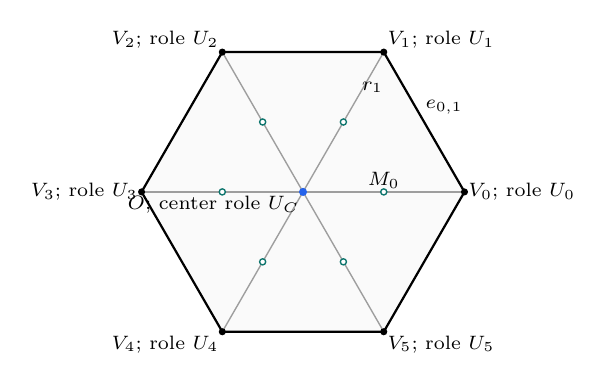
\begin{tikzpicture}[scale=2.05]
  \HexCoords
  \DrawHexagon
  \DrawRays
  \fill[CenterBlue] (O) circle (.025);
  \node[figlabel,below left] at (O) {$O$; center role $U_C$};
  \foreach \i in {0,...,5}{
    \fill (V\i) circle (.022);
    \fill[white,draw=RadialTeal,line width=.5pt]
      ($(O)!.5!(V\i)$) circle (.019);
  }
  \node[figlabel,right] at (V0) {$V_0$; role $U_0$};
  \node[figlabel,above right] at (V1) {$V_1$; role $U_1$};
  \node[figlabel,above left] at (V2) {$V_2$; role $U_2$};
  \node[figlabel,left] at (V3) {$V_3$; role $U_3$};
  \node[figlabel,below left] at (V4) {$V_4$; role $U_4$};
  \node[figlabel,below right] at (V5) {$V_5$; role $U_5$};
  \node[figlabel,above] at ($(O)!.5!(V0)$) {$M_0$};
  \node[figlabel,above right] at ($(O)!.68!(V1)$) {$r_1$};
  \node[figlabel,above right] at ($(V0)!.53!(V1)$) {$e_{0,1}$};
\end{tikzpicture}

\caption{The center, vertices, radial segments, and radial midpoints of $H$.}
\label{fig:geometry-roles}
\end{figure}

For a nonempty compact set $K\subset\mathbb R^2$, define its
\emph{equilateral enclosure side} by
\begin{equation}
 \Lambda(K):=\inf\{s>0:K\subset T\text{ for a closed equilateral
 triangle }T\text{ of side }s\}.
 \label{eq:enclosure-definition}
\end{equation}
Then
\begin{equation}
 \Haus(\partial H)=6,\qquad
 \Haus\left(\bigcup_{i=0}^5r_i\right)=6,\qquad \Haus(S)=12.
\label{eq:target-lengths}
\end{equation}

\begin{theorem}[Main theorem]
\label{thm:main}
The hexagon $H$ cannot be covered by seven open equilateral triangles of side
length one.
\end{theorem}

\begin{corollary}[Soifer's Hexagon Problem]
\label{cor:expanded-closed}
For every $L>1$, the regular hexagon $H_L=LH$ cannot be covered by seven closed
unit equilateral triangles.
\end{corollary}

By \zcref{lem:distinct-roles}, a hypothetical cover has a unique
labeling
\[
 U_C,U_0,\ldots,U_5
\]
such that
\[
 O\in U_C,
 \qquad
 V_i\in U_i.
\]
We call $U_C$ the \emph{C triangle} and $U_i$ the \emph{V triangle at
$V_i$}.  Set
\[
 T_C=\overline{U_C},\qquad T_i=\overline{U_i}.
\]
A \emph{role} means one of these labeled triangles. Statements about an
arrangement of roles assume $O\in U_C$ and $V_i\in U_i$; coverage of
$H$, $S$, or $\partial H$ is an additional hypothesis, stated when needed.
A \emph{skeleton cover} covers $S$, not necessarily all of $H$.
An edge is \emph{center-free} when it is disjoint from $U_C$.

\readerheading{Which part of the hexagon must remain covered?}
A full cover also covers the skeleton $S$. The converse is not assumed.
We retain this weaker target because one later replacement preserves the
skeleton, but need not preserve the interior of $H$. Statements about a
skeleton cover are therefore needed for the logic of the replacement, not
just for estimating lengths. The open sets $U_i$ determine coverage;
their closures $T_i$ are used for maxima, incidence classifications, and
upper bounds. A point of $T_i\setminus U_i$ is not covered by $U_i$.




\subsection{How to read the proof}
Section~\ref{sec:structure-common} introduces the incidence classes, actual
reaches, gaps, and midpoint restrictions, in that order. Its final routing
table gives the exhaustive split after the relevant notation is available.
Sections~\ref{sec:trace-length} and \ref{sec:area-loss} establish the length
and area budgets. Section~\ref{sec:finite-enclosure} explains how to fix
witnesses before testing an arbitrary enclosing triangle; the selected-gap
construction is worked through point by point. Section~\ref{sec:assembly}
assembles the obstructions.

The main text states the geometric inputs and explains their use.
Appendices A--E retain the complete local calculations, including both
replacement charts. Appendix F contains the exact tangent-residual
certificate and identifies its accompanying finite data and replay programs.
Reading a calculation can be postponed, but none is being replaced by an
illustration or an experimental assertion.

\section{Common Geometry and Structural Reductions}
\label{sec:structure-common}
\label{sec:structural-reductions}

We prove the structural facts used by all three mechanisms. The coordinate
calculations are in Appendix~\ref{app:structural-shared-local-signed-center}.

\subsection{Open and closed formulations}

\begin{lemma}[Compact covering margin]
\label{lem:compact-cover-margin}
If a nonempty compact set $K$ is covered by finitely many open unit equilateral
triangles $U_\nu$, then moving every side line inward by the same sufficiently
small positive distance gives a cover by closed equilateral triangles of
side less than one. In particular, $K\subset U$ implies $\Lambda(K)<1$,
with $\Lambda$ defined in \eqref{eq:enclosure-definition}.
\end{lemma}
\begin{proof}
The continuous function
$m(x)=\max_\nu\operatorname{dist}(x,\mathbb R^2\setminus U_\nu)$
has positive minimum $\eta$ on $K$. Move every side line inward by
$0<\rho<\min\{\eta,\sqrt3/6\}$. The resulting closed triangles have
side $1-2\sqrt3\rho$, and each $x\in K$ remains in a triangle realizing
$m(x)\ge\eta>\rho$. Conversely, if $\Lambda(K)<1$, choose a closed
enclosure of side below one and enlarge it about its incenter to side one.
The smaller closed triangle lies in the interior of the enlarged triangle.
\end{proof}

\begin{proposition}[Compactness and scaling equivalence]
\label{prop:open-closed-scaled}
The following assertions are equivalent.
\begin{enumerate}
 \item $H$ is covered by seven open equilateral triangles of side $1$.
 \item For some $\varepsilon>0$, $H$ is covered by seven closed equilateral
 triangles of side $1-\varepsilon$.
 \item For some $L>1$, $H_L:=LH$ is covered by seven closed equilateral
 triangles of side $1$.
\end{enumerate}
\end{proposition}

\begin{proof}
Apply \zcref{lem:compact-cover-margin} to obtain (1)$\Rightarrow$(2).
Enlarging the smaller closed triangles about their incenters gives
(2)$\Rightarrow$(1); dilation by $(1-\varepsilon)^{-1}$ identifies
(2) and (3).
\end{proof}

\begin{lemma}[Distinct triangles]
\label{lem:distinct-roles}
The seven triangles can be labelled so that
\[
 O\in U_C,\qquad V_i\in U_i\quad(0\le i\le5),
\]
and these seven triangles are distinct.  Consequently
\[
 O\in\interior(T_C),\qquad V_i\in\interior(T_i).
\]
\end{lemma}

\begin{proof}
The seven points $O,V_0,\ldots,V_5$ are pairwise at distance at least $1$,
whereas two points of an open unit equilateral triangle are at distance
strictly less than its diameter $1$.  Selecting a covering triangle for each
point therefore gives a bijection.
\end{proof}

\subsection{C triangle and V triangle classifications}

Set
\[
 N_E(T_C):=
 \left\lvert\left\{i\in\mathbb Z/6\mathbb Z:
 \Haus(T_C\cap e_{i,i+1})>0\right\}\right\rvert.
\]
Proposition~\ref{prop:ce-classification} gives $N_E(T_C)\in\{0,1,2\}$;
we call these types $\CEzero,\CEone,\CEtwo$, respectively.

\begin{figure}[H]
\centering
\begin{minipage}[t]{.32\textwidth}
\vspace{0pt}\centering
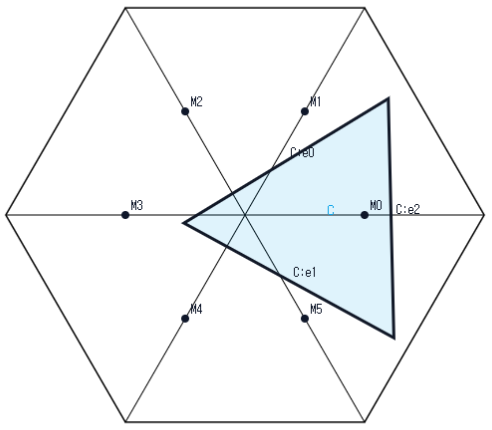
\includegraphics[width=\linewidth,height=.20\textheight,keepaspectratio]
  {figures/role_examples/center_role_ce0_example.png}
\par\smallskip
\footnotesize (a) $\CEzero$
\end{minipage}\hfill
\begin{minipage}[t]{.32\textwidth}
\vspace{0pt}\centering
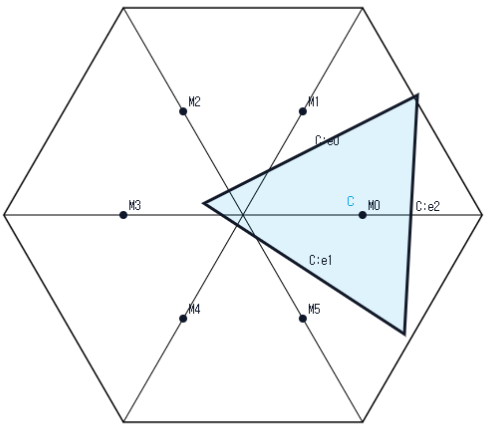
\includegraphics[width=\linewidth,height=.20\textheight,keepaspectratio]
  {figures/role_examples/center_role_ce1_example.png}
\par\smallskip
\footnotesize (b) $\CEone$
\end{minipage}\hfill
\begin{minipage}[t]{.32\textwidth}
\vspace{0pt}\centering
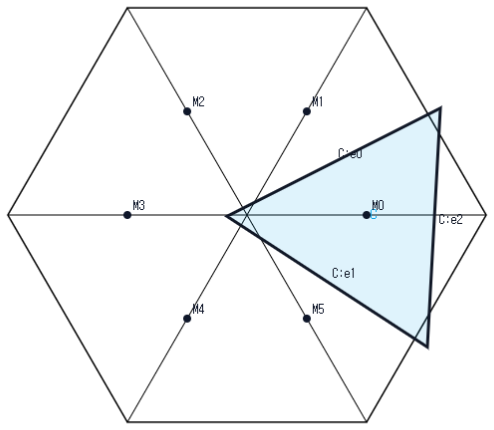
\includegraphics[width=\linewidth,height=.20\textheight,keepaspectratio]
  {figures/role_examples/center_role_ce2_example.png}
\par\smallskip
\footnotesize (c) $\CEtwo$
\end{minipage}
\caption{Examples of the three C triangle classes.  From left to right, the
C triangle has positive-length trace on zero, one, and two edges of
$\partial H$; point contacts do not count.  The panels illustrate the classification.}
\label{fig:center-role-examples}
\end{figure}

Point contacts have zero trace length, so they do not create an additional
positive boundary trace in the definition of $N_E(T_C)$.

\begin{proposition}[Exhaustive center types]
\label{prop:ce-classification}
The closed C triangle $T_C$ has exactly one of the types
$\CEzero,\CEone,\CEtwo$;
equivalently,
\[
 N_E(T_C)\le2.
\]
\end{proposition}

\begin{proof}
If $N_E(T_C)\ge3$, two of the traced edges are nonadjacent in the boundary
six-cycle.  Choose a relative-interior point from each positive-length trace.
By \zcref{lem:app-center-edge-separation}, those points are more than unit
distance apart, so a unit equilateral triangle cannot contain both.
\end{proof}

For the V triangle $T_i$, let $o(T_i)$ be the number of its triangle vertices
outside $H$ and put
\[
 n(T_i)=\left\lvert\left\{j\in\{i-1,i+1\}:
 \Haus(T_i\cap r_j)>0\right\}\right\rvert,
\]
with indices modulo $6$.  The raw pair $(3,0)$ says that all three vertices of
$T_i$ lie outside $H$; it does not say that $T_i$ is disjoint from $H$, since
$V_i\in\interior(T_i)\cap H$.

\begin{lemma}[Local wedge]
\label{lem:local-wedge}
Every original V triangle has $1\le o(T_i)\le3$.  If
$\Haus(T_i\cap r_j)>0$ for some $j\in\{i-1,i+1\}$, at least one vertex of
$T_i$ belongs to $H$; if both adjacent radial traces have positive length,
at least two vertices belong to $H$.
\end{lemma}

\begin{proof}
This is the wedge-incidence calculation in
\zcref{lem:app-local-wedge-calculation}.  The incidence statement concerns the closures; openness is used separately
when forcing points.
\end{proof}

Raw roles with $(o(T_i),n(T_i))=(3,0)$ admit an exact-trace normalization.

\readerheading{Why normalize before measuring reaches?}
The raw case with all three triangle vertices outside $H$ is an incidence
artifact: a translation can leave both its open and closed traces in $H$
unchanged. The next normalization removes that extra case before any actual
reach is defined. It neither enlarges the covered part of $H$ nor changes
which boundary points are covered. This differs from the trace majorant
introduced later, which is not a new open covering triangle.

\begin{proposition}[Exact-trace normalization of raw $(3,0)$ roles]
\label{prop:vd0-exact-trace-normalization}
Let $U$ be an original open V triangle at $V_i$, put $T=\overline U$, and
suppose $(o(T),n(T))=(3,0)$.  There is a same-orientation translate
$\widehat U$, with closure $\widehat T$, such that
\begin{equation}
 V_i\in\widehat U,\qquad (o(\widehat T),n(\widehat T))=(2,0),
 \label{eq:o3-normalized-type}
\end{equation}
and
\begin{equation}
 T\cap H=\widehat T\cap H,\qquad
 U\cap H=\widehat U\cap H.
 \label{eq:o3-exact-traces}
\end{equation}
In particular, all three actual maximal reaches, and whether the two boundary reaches
have sum greater than one, are unchanged.
\end{proposition}

\begin{proof}
The two-orientation affine calculation and the trace-preserving translation
are given in \zcref{lem:app-vd0-trace-normalization-calculation}.
\end{proof}

We apply this translation simultaneously and reuse $U_i,T_i$ for the
normalized triangles.

The normalized exhaustive types used below are
\[
\begin{array}{c|c}
(o(T_i),n(T_i))&\text{established type}\\ \hline
(1,0)&\Vdzero\\
(2,0)&\Vdzero\\
(1,1)&\Vdone\\
(1,2)&\Vdtwo\\
(2,1)&\Tlike.
\end{array}
\]

\begin{proposition}[Exhaustive normalized vertex types]
\label{prop:vertex-classification}
Every normalized V triangle has exactly one of the four types
$\Vdzero,\Vdone,\Vdtwo,\Tlike$ in the displayed type dictionary.
\end{proposition}

\begin{proof}
Lemma~\ref{lem:local-wedge} gives $o\le2$ when $n\ge1$ and $o\le1$ when
$n=2$, while $o\ge1$.  Proposition
\ref{prop:vd0-exact-trace-normalization} replaces the only additional raw
pair, $(3,0)$, by $(2,0)$.
\end{proof}

The next construction is a trace majorant, not a new open covering triangle.

\begin{proposition}[T3-like closed-trace domination]
\label{prop:t3-translation}
Let $T$ be the closure of an original $\Tlike$ V triangle at $V_i$.  There is
a same-orientation translate $\widehat T$ such that
\[
 V_i\in\operatorname{relint}(\text{a side of }\widehat T),
 \qquad T\cap H\subsetneq\widehat T\cap H,
\]
and $(o(\widehat T),n(\widehat T))=(2,1)$, while
\[
 \interior(T)\cap(H\setminus\{V_i\})\subseteq\interior(\widehat T).
\]
Since $V_i$ becomes a boundary point, $\widehat T$ is only a closed-trace
majorant.
\end{proposition}

\begin{proof}
See the two-orientation feasibility calculation in
\zcref{lem:app-t3-translation-calculation}.
\end{proof}

\subsection{Initial reaches and boundary gaps}

The actual maximal reaches are
\[
 A_i:=\max\{x\in[0,1]:V_i+x(V_{i-1}-V_i)\in T_i\},
\]
\[
 B_i:=\max\{x\in[0,1]:V_i+x(V_{i+1}-V_i)\in T_i\},
\]
\[
 C_i:=\max\{x\in[0,1]:V_i+x(O-V_i)\in T_i\}.
\]
The same numbers are the suprema of the corresponding reaches in the open
triangle $U_i$. The V triangle $T_i$ is \emph{supercritical} when
$A_i+B_i>1$, and \emph{nonsupercritical} when $A_i+B_i\le1$. Put
\begin{equation}
 N_+:=\left\lvert\left\{i\in\mathbb Z/6\mathbb Z:
 A_i+B_i>1\right\}\right\rvert.
 \label{eq:N-plus-definition}
\end{equation}
Lowercase reaches are used only after a selection satisfying
\[
 0\le a_i\le A_i,\qquad 0\le b_i\le B_i,\qquad 0\le c_i\le C_i.
\]
They never define $N_+$.

\begin{lemma}[Initial reach segments]
\label{lem:reach-initial-segments}
On the three segments from $V_i$ toward $V_{i-1},V_{i+1},O$, the closed
parameter sets are respectively
\[
 [0,A_i],\qquad[0,B_i],\qquad[0,C_i],
\]
and the open parameter sets are
\[
 [0,A_i),\qquad[0,B_i),\qquad[0,C_i).
\]
Thus the closed maxima equal the corresponding open-triangle suprema.
\end{lemma}

\begin{proof}
The other endpoint of each segment is a distinguished point at distance
one from $V_i$, and is not even in $T_i$: otherwise moving $V_i$
slightly away from it inside $U_i$ would exceed diameter one.
Thus $0<A_i,B_i,C_i<1$. Each intersection with a segment issuing from
$V_i$ is convex.  Closedness of $T_i$, openness of $U_i$, and
$T_i=\overline{U_i}$ give the stated endpoints.
\end{proof}

Parametrize $e_{i,i+1}$ from $V_i$ to $V_{i+1}$ by
\[
 X_i(x):=V_i+x(V_{i+1}-V_i),\qquad 0\le x\le1.
\]
Define the \emph{boundary gap}
\[
 J_i:=e_{i,i+1}\setminus(U_i\cup U_{i+1}),\qquad
 N_{\mathrm{gap}}:=|\{i:J_i\ne\varnothing\}|.
\]
Lemma~\ref{lem:gap-exhaustion} gives
$J_i=X_i([B_i,1-A_{i+1}])$ when $B_i+A_{i+1}\le1$, and $J_i=\varnothing$
otherwise. Equality is a singleton gap, not an overlap.

\begin{lemma}[Exhaustiveness of the gap split]
\label{lem:gap-exhaustion}
One has
\[
 J_i=\begin{cases}
 X_i([B_i,1-A_{i+1}]),&B_i+A_{i+1}\le1,\\
 \varnothing,&B_i+A_{i+1}>1.
 \end{cases}
\]
Every nonempty gap, including a singleton, is missed by all open V triangles.
Under a hypothetical cover it lies in $U_C$ and creates a positive-length
C triangle trace.
Consequently a closed C triangle $T_C$ of type
$\CEzero,\CEone,\CEtwo$ permits respectively at most $0,1,2$ gaps, and
\[
 N_{\mathrm{gap}}=0
 \iff U_0,\ldots,U_5\text{ cover }\partial H.
\]
\end{lemma}

\begin{proof}
By \zcref{lem:reach-initial-segments}, the incident open traces have
parameters $[0,B_i)$ and $(1-A_{i+1},1]$. Their complement is the stated
closed interval.
A nonincident V triangle cannot contain a relative-interior point of the edge:
that point is more than unit distance from its distinguished vertex.  Hence a
gap lies in $U_C$; openness turns even a singleton V-gap into a
positive-length C trace.  Proposition~\ref{prop:ce-classification} gives the
count and the final equivalence.
\end{proof}

\readerheading{Why the threshold is one.}
On a gap-free edge, the open traces overlap, so $B_i+A_{i+1}>1$.
If every edge is gap-free, summing gives
\[
 6<\sum_{i=0}^5(B_i+A_{i+1})=\sum_{i=0}^5(A_i+B_i).
\]
At least one V triangle must therefore be supercritical. A nonempty gap
breaks this cyclic argument: it is precisely where the C triangle takes
over a boundary obligation. Equality $B_i+A_{i+1}=1$ still leaves the
common endpoint uncovered by the two open V triangles; it belongs to the
gap branch, not to the overlap branch.

The distinction between actual and selected reaches is also geometric.
The numbers $A_i,B_i,C_i$ describe a fixed triangle. The later lower bounds
$a_i,b_i,c_i$ prescribe points it must contain and may be reduced when making
a common comparison. Reducing a demand does not change the original
triangle or the count $N_+$.


\begin{lemma}[T3-like V triangles are nonsupercritical]
\label{lem:t3-nonsupercritical}
Every original $\Tlike$ V triangle satisfies
\begin{equation}
 A_i+B_i\le1.
 \label{eq:t3-nonsupercritical}
\end{equation}
Moreover $M_i\notin T_i$. In particular, a T3-like role is not counted
by $N_+$ and cannot supply its own midpoint.
\end{lemma}

\begin{proof}
Both assertions follow from the Type-II calculation in
\zcref{lem:app-t3-translation-calculation}.
\end{proof}

A V role has \emph{positive adjacent-radial support}, or simply
\emph{positive support}, when $n(T_i)>0$. Put
\[
 N_{\mathrm{sp}}:=|\{i:n(T_i)>0\}|.
\]
Positive-support roles are nonsupercritical, so the number of roles that
are supercritical or have positive adjacent-radial support is
$N_++N_{\mathrm{sp}}$. The skeleton budget excludes nonzero-gap covers
with $N_++N_{\mathrm{sp}}\ge3$.

\begin{figure}[H]
\centering
\begin{minipage}[t]{.32\textwidth}
\vspace{0pt}\centering
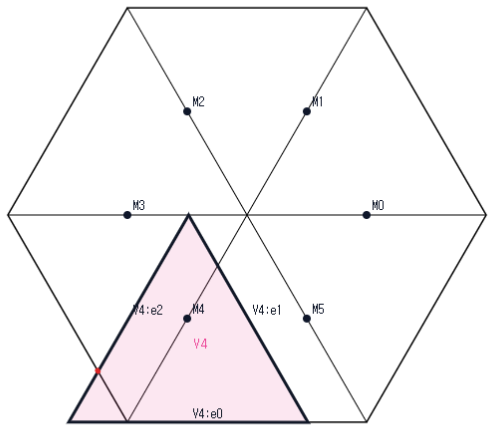
\includegraphics[width=\linewidth,height=.22\textheight,keepaspectratio]
  {figures/role_examples/vertex_role_vd0_axis_aligned_example.png}
\par\smallskip
\footnotesize (a) axis-aligned $\Vdzero$
\end{minipage}\hfill
\begin{minipage}[t]{.32\textwidth}
\vspace{0pt}\centering
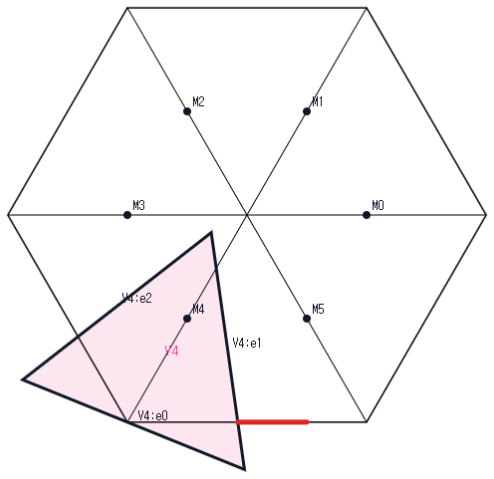
\includegraphics[width=\linewidth,height=.22\textheight,keepaspectratio]
  {figures/role_examples/vertex_role_vd0_nonsupercritical_example.png}
\par\smallskip
\footnotesize (b) nonsupercritical $\Vdzero$
\end{minipage}\hfill
\begin{minipage}[t]{.32\textwidth}
\vspace{0pt}\centering
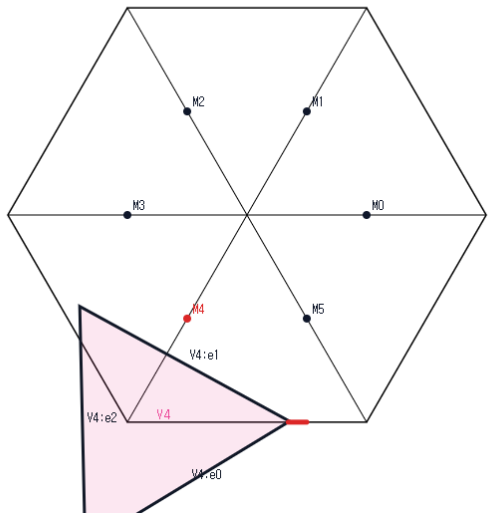
\includegraphics[width=\linewidth,height=.22\textheight,keepaspectratio]
  {figures/role_examples/vertex_role_vd0_supercritical_example.png}
\par\smallskip
\footnotesize (c) supercritical $\Vdzero$
\end{minipage}
\par\medskip
\begin{minipage}[t]{.32\textwidth}
\vspace{0pt}\centering
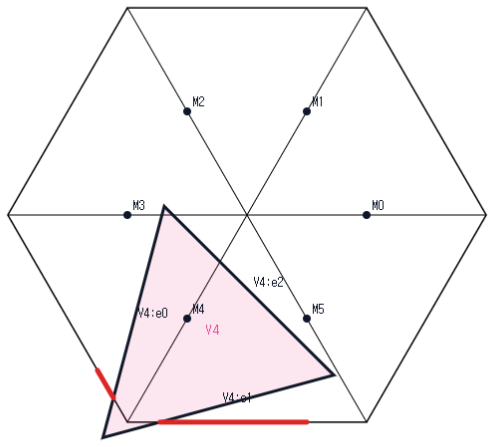
\includegraphics[width=\linewidth,height=.22\textheight,keepaspectratio]
  {figures/role_examples/vertex_role_vd1_example.png}
\par\smallskip
\footnotesize (d) $\Vdone$
\end{minipage}\hfill
\begin{minipage}[t]{.32\textwidth}
\vspace{0pt}\centering
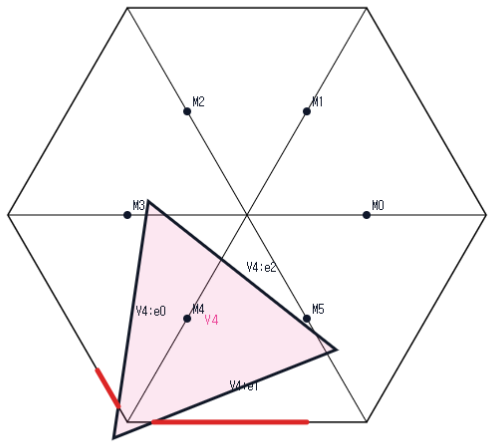
\includegraphics[width=\linewidth,height=.22\textheight,keepaspectratio]
  {figures/role_examples/vertex_role_vd2_example.png}
\par\smallskip
\footnotesize (e) $\Vdtwo$
\end{minipage}\hfill
\begin{minipage}[t]{.32\textwidth}
\vspace{0pt}\centering
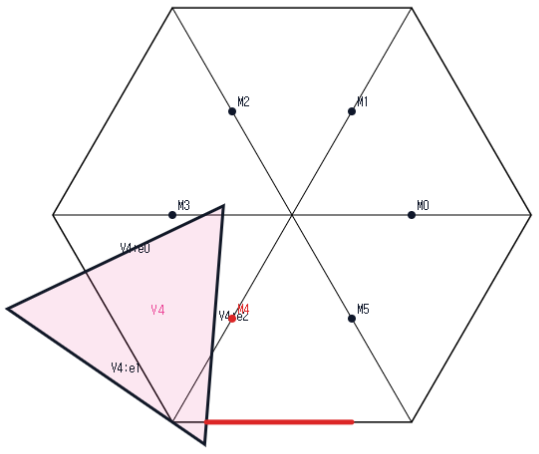
\includegraphics[width=\linewidth,height=.22\textheight,keepaspectratio]
  {figures/role_examples/vertex_role_t3_like_example.png}
\par\smallskip
\footnotesize (f) $\Tlike$
\end{minipage}
\caption{Examples of the normalized V triangle types.  The top row shows an
axis-aligned $\Vdzero$, a nonsupercritical $\Vdzero$ with $A_i+B_i\le1$,
and a supercritical $\Vdzero$ with $A_i+B_i>1$.  The bottom row shows
$\Vdone$, $\Vdtwo$, and $\Tlike$.  The panels illustrate the classification.}
\label{fig:vertex-role-examples}
\end{figure}

\subsection{Strict handoffs and midpoint forcing}

\begin{proposition}[Strict boundary handoffs]
\label{prop:strict-handoffs}
Assume that $U_0,\ldots,U_5$ cover $\partial H$.  There are choices
\[
 \xi_i\in(1-A_{i+1},B_i),\qquad
 a_i:=1-\xi_{i-1},\qquad b_i:=\xi_i,
\]
such that
\[
 0<a_i<A_i,\qquad0<b_i<B_i,\qquad
 a_i^2+a_ib_i+b_i^2<1.
\]
The selected anchors lie in $U_i$.  If exactly one actual V triangle is
supercritical, every strict selection has that same unique selected
supercritical index.  If at least two actual V triangles are supercritical,
some simultaneous strict selection retains at least two.
\end{proposition}

\begin{proof}
The overlap intervals and the cyclic selector are proved in
\zcref{lem:app-strict-handoff-selection}.  Geometrically, each $\xi_i$ lies
in the overlap of two adjacent open edge traces, which makes both associated
reach demands strict.
\end{proof}

\begin{lemma}[Boundary deficit and overlap identities]
\label{lem:boundary-deficit-identities}
For the actual reaches put $s_i=1-A_i-B_i$ and
$\omega_i=B_i+A_{i+1}-1$. Then
\[
 A_{i+1}-A_i=s_i+\omega_i,\qquad
 B_i-B_{i+1}=s_{i+1}+\omega_i.
\]
On a nonsupercritical gap-free path the $A_i$ increase and the $B_i$
decrease strictly. Weak handoffs give the weak version. Around the full
cycle, $\sum_i\omega_i=-\sum_i s_i$.
\end{lemma}
\begin{proof}
Expand the definitions and telescope. Nonsupercriticality gives $s_i\ge0$,
and a gap-free edge has $\omega_i>0$ because its incident traces are open.
A supercritical role has $s_i<0$; propagation through it is not licensed.
\end{proof}

\begin{lemma}[Self-midpoint obstruction]
\label{lem:self-midpoint}
Let $u,v$ be unit vectors meeting at $120^\circ$, and let $a,b\in[0,1]$.
If a closed unit
equilateral triangle contains
\[
 0,\qquad au,\qquad bv,\qquad\frac{u+v}{2},
\]
then $a+b\le1$.  Consequently
\[
 M_i\in T_i\Longrightarrow A_i+B_i\le1.
\]
If the boundary points and midpoint are contained with positive margin, the
conclusion is strict.
\end{lemma}

\begin{proof}
This is the admissible-set corollary
\zcref{lem:app-self-midpoint-caliper}.
\end{proof}

\begin{proposition}[CE1/CE2 exactly-one-midpoint property]
\label{prop:unique-center-midpoint}
If $O\in\interior(T_C)$ and $T_C$ is $\CEone$ or $\CEtwo$, then
\[
 \left|T_C\cap\{M_0,\ldots,M_5\}\right|=1.
\]
This midpoint belongs to $U_C$. Both possible positive boundary traces
are on the two hexagon edges incident to the same vertex.
\end{proposition}

\begin{proof}
Normalize one positive boundary trace.  The signed-center optimization
\zcref{prop:signed-center-normal-form} gives the exact midpoint set
$\{M_0\}$, with radial exit $d_0^C>1/2$ and positive side slacks at
$M_0$. Its boundary traces are confined to $e_{5,0},e_{0,1}$.
Undoing the symmetry proves the assertions.
\end{proof}

The interior hypothesis is essential: $\conv\{O,V_0,V_1\}$ has a boundary
edge overlap and contains both $M_0$ and $M_1$, but $O$ is not interior to it.

\subsection{Exhaustive routing}

When the C triangle has type CE1 or CE2, \zcref{prop:unique-center-midpoint}
shows that it contains exactly one of $M_0,\ldots,M_5$; this is the
\emph{C midpoint}. If it is $M_k$, the role at $V_k$ is called
\emph{center-based}; a supercritical role there is \emph{center-aligned},
and a role at another vertex is \emph{away} or \emph{off-center}.
A V role that contains an adjacent midpoint openly is
called its \emph{supplier} or \emph{rescuer}. A \emph{gap-free
nonsupercritical path} is a consecutive sequence of nonsupercritical V
roles whose shared edges have empty gaps.

We use BC for the selected-gap six-point construction, D for the supported-
midpoint four-point construction, and F for the zero-gap nine-point
construction, all defined in Section~\ref{sec:finite-enclosure}.
N0 denotes \zcref{thm:fixed-nzero}, the assertion that every skeleton
cover has a supercritical V role.

Zero gaps mean that the V triangles cover $\partial H$, and the proof
splits according to $N_+$. With a gap, the C triangle is CE1 or CE2;
N0 and the skeleton budget leave one supercritical role and at most one
positive-support role. Its position relative to the C midpoint determines
the remaining obstruction.

\begin{table}[H]
\centering\small
\setlength{\tabcolsep}{5pt}\renewcommand{\arraystretch}{1.15}
\begin{tabular}{@{}ccp{.34\textwidth}p{.28\textwidth}@{}}
\toprule
$N_{\rm gap}$&$N_+$&Additional condition&Closing mechanism\\
\midrule
$0$&$0$&Arbitrary V types&Strict overlap\\
$0$&$1$&Arbitrary V types&Nine-point F\\
$0$&$\ge2$&Arbitrary V types&Cyclic area loss\\
\midrule
$\ge1$&$0$&Arbitrary V types&N0, through BC\\
$\ge1$&$\ge1$&$N_+\ge2$ or $N_++N_{\rm sp}\ge3$&Skeleton budget\\
$\ge1$&$1$&$N_{\rm sp}\le1$&Midpoint supplier: BC, D, replacement, or Vd2 length\\
\bottomrule
\end{tabular}
\caption{Disjoint routes for the original open cover. Nonzero gaps force
CE1 or CE2; both classes share the same placement reduction. Replacement
preserves the skeleton and ends at N0, without preserving number of gaps.}
\label{tab:routing}
\end{table}

The rows are disjoint and exhaustive: separate zero from nonzero gaps,
then $N_+=0$, and finally the displayed high-count condition.
Lemma~\ref{lem:midpoint-supplier} resolves the last row. BC uses the same
selected-gap witness in CE1 and CE2, with separate candidate calculations.

\section{Trace-Length Mechanism}
\label{sec:trace-length}
\label{sec:length}

For a closed triangle $T$ and a rectifiable target $E$, define
\[
 L_E(T):=\Haus(T\cap E).
\]
\begin{lemma}[Connected open-cover budget]
\label{lem:open-cover-budget}
Let $X$ be compact and connected, with a finite Borel measure $\mu$
positive on every nonempty relatively open subset. For a finite open cover
with at least two nonempty relative pieces,
\[
 \mu(X)<\sum_j\mu(U_j\cap X)\le\sum_j\mu(T_j\cap X).
\]
Consequently closed-piece upper bounds whose sum is at most $\mu(X)$
already contradict the open cover.
\end{lemma}
\begin{proof}
If the nonempty relative pieces were pairwise disjoint, one and the union
of the others would disconnect $X$. Some pair therefore overlaps in a
nonempty relatively open set, of positive measure. Integrating the covering
multiplicity gives strict inequality. Closure only enlarges each piece.
\end{proof}

For $X=\partial H$ or $S$, use length; for $X=H$, use area. Each measure
has the stated full-support property, and the seven distinguished roles
meet the corresponding targets in positive measure. In particular,
\begin{equation}
 \Haus(E)<L_E(T_C)+\sum_{i=0}^5L_E(T_i),\qquad E\in\{\partial H,S\},
 \label{eq:length-subadditivity}
\end{equation}
whenever these targets are covered. Empty center boundary traces are simply
omitted from the collection. The local geometric caps remain separate from
this common final budget argument.

\begin{figure}[H]
\centering
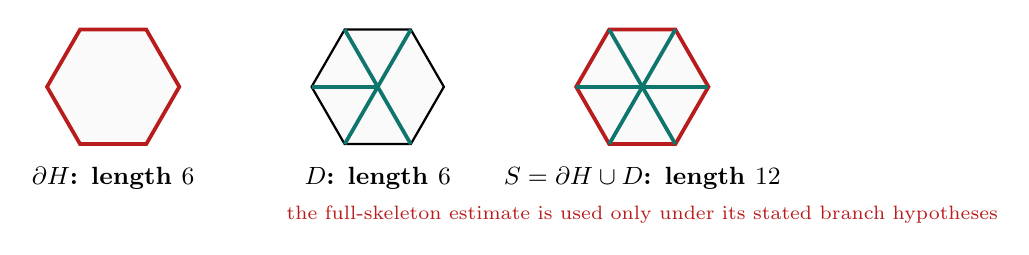
\begin{tikzpicture}[scale=.84]
  \foreach \x/\title in {0/$\partial H$: length $6$,4/$D$: length $6$,8/$S=\partial H\cup D$: length $12$}{
    \begin{scope}[xshift=\x cm]
      \coordinate (a0) at (1,0);
      \coordinate (a1) at (.5,.866);
      \coordinate (a2) at (-.5,.866);
      \coordinate (a3) at (-1,0);
      \coordinate (a4) at (-.5,-.866);
      \coordinate (a5) at (.5,-.866);
      \coordinate (o) at (0,0);
      \draw[hex] (a0)--(a1)--(a2)--(a3)--(a4)--(a5)--cycle;
      \node[panellabel,align=center] at (0,-1.38) {\title};
    \end{scope}
  }
  \draw[demand] (1,0)--(.5,.866)--(-.5,.866)--(-1,0)--(-.5,-.866)--(.5,-.866)--cycle;
  \foreach \p in {(4,0),(4.5,.866),(3.5,.866),(3,0),(3.5,-.866),(4.5,-.866)}{
    \draw[radialdemand] (4,0)--\p;
  }
  \draw[demand] (9,0)--(8.5,.866)--(7.5,.866)--(7,0)--(7.5,-.866)--(8.5,-.866)--cycle;
  \foreach \p in {(9,0),(8.5,.866),(7.5,.866),(7,0),(7.5,-.866),(8.5,-.866)}{
    \draw[radialdemand] (8,0)--\p;
  }
  \node[figlabel,align=center,text=DemandRed] at (8,-1.93)
    {the full-skeleton estimate is used only under its stated branch hypotheses};
\end{tikzpicture}

\caption{The perimeter and full-skeleton targets.  The skeleton is used only
under the hypotheses of the corresponding trace budget.}
\label{fig:strategy1-targets}
\end{figure}

\subsection{Skeleton interfaces}

\begin{lemma}[Center skeleton cap]
\label{lem:center-skeleton-cap}
If $N_E(T_C)\in\{1,2\}$ and
\[
 \left|T_C\cap\{M_0,\ldots,M_5\}\right|=1,
\]
then
\[
 L_S(T_C)<\frac32.
\]
\end{lemma}

\begin{proof}
This is the signed-center trace optimization
\zcref{lem:app-center-skeleton-cap-calculation}.
\end{proof}

\begin{lemma}[Positive-support skeleton cap]
\label{lem:positive-support-skeleton-cap}
Let $T_i$ be the closure of an original open V triangle.  If
\[
 \exists j\in\{i-1,i+1\}\quad\Haus(T_i\cap r_j)>0,
\]
then
\[
 L_S(T_i)<\frac32.
\]
\end{lemma}

\begin{proof}
Normalize to $i=0$ and translate the hexagon by $V_0$.  The five components
of $S$ on which a unit triangle containing $V_0$ can have positive trace
become the corresponding local components of the translated skeleton.  The
positive adjacent-radial trace becomes a positive boundary trace there.
Proposition~\ref{prop:unique-center-midpoint} and
Lemma~\ref{lem:center-skeleton-cap} give the bound; every nonlocal component
is more than unit distance from $V_0$, apart from zero-measure endpoints.
\end{proof}

\begin{lemma}[No-support skeleton cap]
\label{lem:no-support-skeleton-cap}
If
\[
 A_i+B_i\le1,
\]
\[
 \Haus(T_i\cap r_{i-1})=0,
 \qquad \Haus(T_i\cap r_{i+1})=0,
\]
then
\[
 L_S(T_i)\le2.
\]
\end{lemma}

\begin{proof}
See \zcref{lem:app-no-support-skeleton-calculation}; geometrically, the two
incident boundary traces and the own radial trace are the only components
that can contribute positive length.
\end{proof}

\begin{lemma}[Supercritical skeleton cap]
\label{lem:supercritical-skeleton-cap}
If $A_i+B_i>1$, then
\[
 L_S(T_i)<\frac32.
\]
\end{lemma}

\begin{proof}
The exact admissible-cell and polynomial-sign calculation is
\zcref{lem:app-supercritical-skeleton-calculation}.
\end{proof}

\begin{lemma}[Positive-support rescuer]
\label{lem:positive-support-rescuer}
Suppose $N_E(T_C)\in\{1,2\}$ and, after symmetry,
\[
 T_C\cap\{M_0,\ldots,M_5\}=\{M_0\}.
\]
If $N_+\ge2$, then for a supercritical index $s\ne0$ there is
$j\in\{s-1,s+1\}$ such that
\[
 M_s\in U_j,
 \qquad \Haus(T_j\cap r_s)>0.
\]
\end{lemma}

\begin{proof}
Choose a supercritical $s\ne0$.  Lemma~\ref{lem:self-midpoint} gives
$M_s\notin T_s$, and the displayed midpoint identity gives
$M_s\notin T_C$.  The open cover therefore puts $M_s$ in another $U_j$.
Diameter locality restricts $j$ to $s-1$ or $s+1$, and openness makes its
trace on $r_s$ have positive length.
\end{proof}

\begin{theorem}[Direct CE1/CE2 skeleton count]
\label{thm:common-skeleton-count}
If
\[
 N_E(T_C)\in\{1,2\},
\]
\[
 \left|T_C\cap\{M_0,\ldots,M_5\}\right|=1,
\]
and
\begin{equation}
 N_++N_{\mathrm{sp}}\ge3,
 \label{eq:common-skeleton-count}
\end{equation}
then the seven triangles do not cover $S$.
\end{theorem}

\begin{proof}
The three geometric caps above make the total trace strictly smaller than
$\Haus(S)=12$; the exact budget is
\zcref{lem:app-common-skeleton-count-calculation}.  This contradicts
\eqref{eq:length-subadditivity}.
\end{proof}

\subsection{Boundary trace register}

The exact evaluation is in Appendix~\ref{app:trace-length-optimization}; the
following table is the complete interface used by the routing argument.

\begin{theorem}[Boundary trace table]
\label{thm:boundary-trace-table}
For closures of original open triangles, the following bounds hold.
\begingroup
\setlength{\arraycolsep}{5pt}
\renewcommand{\arraystretch}{1.18}
\begin{equation}
\begin{array}{c|c|c}
\text{exact hypothesis}&\text{established class}&\text{exact bound}\\ \hline
N_E(T_C)=0&\CEzero&L_{\partial H}(T_C)=0\\
N_E(T_C)=1&\CEone&
 L_{\partial H}(T_C)\le\dfrac{\sqrt3}{2}-\dfrac34\\[3pt]
N_E(T_C)=2&\CEtwo&L_{\partial H}(T_C)<\dfrac12\\[3pt]
\begin{gathered}
 (o(T_i),n(T_i))\in\{(1,0),(2,0)\}\\
 A_i+B_i\le1
\end{gathered}
 &\Vdzero&L_{\partial H}(T_i)\le1\\[8pt]
\begin{gathered}
 (o(T_i),n(T_i))\in\{(1,0),(2,0)\}\\
 A_i+B_i>1
\end{gathered}
 &\Vdzero&L_{\partial H}(T_i)\le\dfrac2{\sqrt3}\\[8pt]
(o(T_i),n(T_i))\in\{(1,1),(1,2)\}
 &\Vdone\text{ or }\Vdtwo&L_{\partial H}(T_i)<\dfrac12\\
(o(T_i),n(T_i))=(2,1)&\Tlike&L_{\partial H}(T_i)<1.
\end{array}
\label{eq:boundary-trace-table}
\end{equation}
\endgroup
For every V triangle,
\begin{equation}
 L_{\partial H}(T_i)=A_i+B_i.
 \label{eq:vertex-boundary-locality}
\end{equation}
\end{theorem}

\begin{proof}
The locality identity and every row are proved in
\zcref{lem:app-boundary-trace-table-calculation}.
\end{proof}

\begin{corollary}[Branches closed by the common budgets]
\label{cor:signed-budget-branches}
The following exact alternatives are impossible.
\begin{enumerate}
\item $N_E(T_C)=0$, $N_+=1$, and $d\ge1$;
\item $N_E(T_C)\in\{1,2\}$, $N_+=0$, and $d\ge1$;
\item $N_E(T_C)=1$, $N_+=1$, and $d\ge1$;
\item $N_E(T_C)=2$, $N_+=1$, and $d\ge2$;
\item $N_E(T_C)=2$, $N_+=1$, and there is an index $i$ such that
\[
 (o(T_i),n(T_i))=(1,2)
\]
and
\[
 \{M_{i-1},M_{i+1}\}\cap T_i\ne\varnothing;
\]
\item $N_E(T_C)\in\{1,2\}$ and $N_++N_{\mathrm{sp}}\ge3$;
\item $N_E(T_C)\in\{1,2\}$ and $N_+\ge2$.
\end{enumerate}
\end{corollary}

\begin{proof}
The perimeter sums for items (1)--(5) are
\zcref{lem:app-signed-budget-calculation}.  Item (6) is
Theorem~\ref{thm:common-skeleton-count}.  For item (7), normalize the unique
C triangle midpoint and apply Lemma~\ref{lem:positive-support-rescuer}; its
rescuer is distinct from the two supercritical triangles, so item (6)
applies.
\end{proof}

\begin{proposition}[Vd2 adjacent-midpoint branch]
\label{prop:ce2-vd2-midpoint-length}
Suppose the C triangle is CE1 or CE2 and $N_+=1$. If a Vd2 role contains
an adjacent midpoint, the perimeter is not covered.
\end{proposition}
\begin{proof}
By \zcref{lem:vd2-neighbor-midpoint-cap}, that role contributes strictly
less than $1/3$. The common boundary caps give
\[
 L_{\partial H}(T_C)+\sum_iL_{\partial H}(T_i)
 <\frac12+\frac2{\sqrt3}+\frac13+4<6.
\]
Apply \zcref{lem:open-cover-budget}. The argument needs no CE2-only formula.
\end{proof}

\subsection{Routing conclusion}

The zero-gap $N_+=1$, $d\ge1$ clause is retained as an independent
alternative; the routing table now sends every zero-gap $N_+=1$ state to
\zcref{thm:reader-zero-gap-obstruction}.

\begin{proposition}[Branches closed by the trace-length mechanism]
\label{prop:length-branches}
The following routing entries and hybrid subcase are impossible.
\begin{enumerate}
 \item $N_{\mathrm{gap}}=0$ and $N_+=0$;
 \item $N_{\mathrm{gap}}=0$, $N_+=1$, and $d\ge1$;
 \item $N_E(T_C)\in\{1,2\}$ and $N_++N_{\mathrm{sp}}\ge3$;
 \item $N_E(T_C)\in\{1,2\}$, $N_+=0$, and $d\ge1$;
 \item $N_E(T_C)=1$, $N_+=1$, and $(d,t)=(1,0)$;
 \item the subcase of $N_E(T_C)=2$, $N_+=1$, and $(d,t)=(1,0)$ in which
 the unique non-$\Vdzero$ triangle $T_i$ satisfies
 \[
  (o(T_i),n(T_i))=(1,2)
 \]
 and
 \[
  \{M_{i-1},M_{i+1}\}\cap T_i\ne\varnothing.
 \]
\end{enumerate}
\end{proposition}

\begin{proof}
For item (1), Lemma~\ref{lem:gap-exhaustion} makes the incident open V
traces overlap on every edge, so
\[
 B_i+A_{i+1}>1\qquad(0\le i\le5).
\]
Summing contradicts $N_+=0$.  Items (2)--(5) are clauses (1), (6), (2), and
(3), respectively, of Corollary~\ref{cor:signed-budget-branches}; their
numerical budgets are evaluated in Appendix~\ref{app:trace-length-optimization}.
Item (6) is Proposition~\ref{prop:ce2-vd2-midpoint-length}.
\end{proof}

\section{Area-Loss Estimate}
\label{sec:area-loss}

The area-loss method records how much of each V triangle must lie outside
$H$.  The local estimate applies to every V triangle. A final cyclic argument
adds these losses without imposing a center type.

Put $A_\triangle=\sqrt3/4$ and normalize all areas by $A_\triangle$.  At
$V_0$ define
\[
 \mathcal T(a,b):=
 \left\{T:\begin{array}{l}
 T\text{ is a closed unit equilateral triangle},\\
 \{V_0,V_0+a(V_5-V_0),V_0+b(V_1-V_0)\}\subseteq T
 \end{array}\right\},
\]
\[
 \mathcal L(T):=\frac{\operatorname{area}(T\setminus H)}{A_\triangle},
 \qquad
 \mathcal L(a,b):=\inf_{T\in\mathcal T(a,b)}\mathcal L(T),
\]
where $a,b\in[0,1]$ and $\mathcal T(a,b)\ne\varnothing$.  Hexagon
symmetry gives the corresponding family at every $V_i$.  In particular,
if
\[
 0\le a_i\le A_i,
 \qquad
 0\le b_i\le B_i,
\]
then the rotated copy of $T_i$ belongs to $\mathcal T(a_i,b_i)$.

\begin{figure}[H]
\centering
\begin{minipage}[b]{.48\textwidth}
\centering
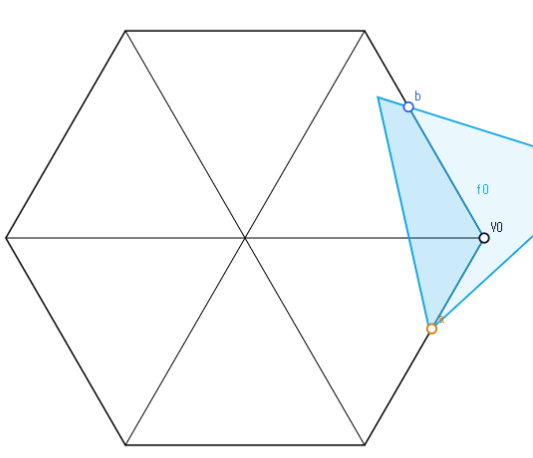
\includegraphics[width=\linewidth]
  {figures/strategy3_local_area_loss.png}
\par\smallskip
\footnotesize (a) local retained area
\end{minipage}\hfill
\begin{minipage}[b]{.48\textwidth}
\centering
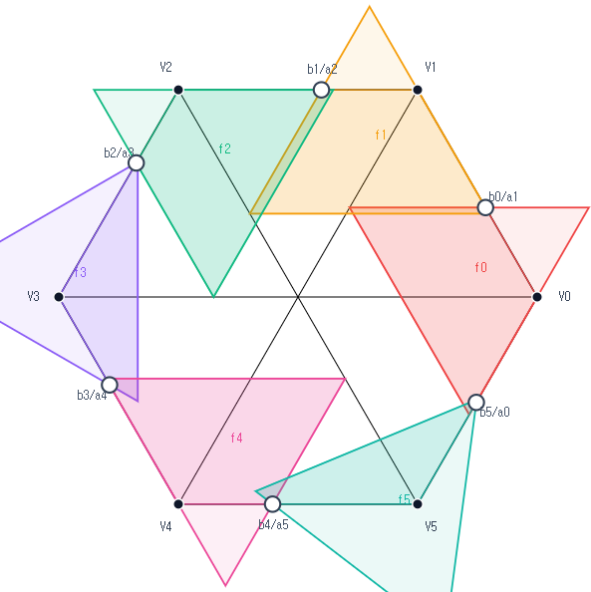
\includegraphics[width=\linewidth]
  {figures/strategy3_global_area_loss.png}
\par\smallskip
\footnotesize (b) cyclic retained areas
\end{minipage}
\caption{The area-loss method.  The dark regions indicate the portions
retained in $H$; the exact quantities are $\mathcal L(T)$ and
$\mathcal L(a,b)$.}
\label{fig:area-loss}
\end{figure}

\subsection{Local area loss}

\begin{theorem}[Local square loss]
\label{thm:local-square-loss}
For every feasible $(a,b)$,
\begin{equation}
 \mathcal L(a,b)\ge\min\{a,b\}^2.               \label{eq:min-square-loss}
\end{equation}
If $a+b>1$, then
\begin{equation}
 \mathcal L(a,b)\ge\max\{a,b\}^2.               \label{eq:max-square-loss}
\end{equation}
The same bounds hold for every $T\in\mathcal T(a,b)$.
\end{theorem}

\begin{proof}
The two exhaustive orientation families give these minima.  Their polygon
areas and the factorizations proving both inequalities are computed in
\zcref{lem:appendix-local-square-loss}.
\end{proof}

\subsection{Cyclic accumulation}

Use the strict handoffs from \zcref{prop:strict-handoffs}:
\[
 \xi_i\in(1-A_{i+1},B_i),
 \qquad
 a_i:=1-\xi_{i-1},
 \qquad
 b_i:=\xi_i.
\]
They satisfy
\[
 0<a_i<A_i,
 \qquad
 0<b_i<B_i,
 \qquad
 a_i^2+a_ib_i+b_i^2<1.
\]

\begin{lemma}[Cyclic area-loss certificate]
\label{lem:cyclic-area-loss}
The six actual V triangles satisfy
\[
 \left|\{i\in\mathbb Z/6\mathbb Z:a_i+b_i>1\}\right|\ge2
 \quad\Longrightarrow\quad
 \sum_{i=0}^5\mathcal L(T_i)>1.
\]
\end{lemma}

\begin{proof}
Apply the local bounds around the six-cycle.  The exact sum, including
the strict contribution from the second ascent, are given in
\zcref{lem:appendix-cyclic-area-loss}.
\end{proof}

\begin{proposition}[Branch closed by area]
\label{prop:area-branches}
The branch $N_{\rm gap}=0$, $N_+\ge2$ is impossible.
\end{proposition}
\begin{proof}
The six V triangles cover $\partial H$. The at-least-two clause of
\zcref{prop:strict-handoffs} supplies the selection for
\zcref{lem:cyclic-area-loss}. Thus the V triangles have total normalized
inside area below five. The C triangle contributes at most one, whereas
$H$ has normalized area six. Apply \zcref{lem:open-cover-budget} with area.
\end{proof}

\section[Finite-Enclosure Method]{Finite-Enclosure Obstructions}
\label{sec:finite-enclosure}

The finite-enclosure method identifies a compact set that the C triangle
must contain, then proves that this set does not fit inside any open unit
equilateral triangle.

Put
\[
 h:=\frac{\sqrt3}{2}.
\]

The closed-disk notation and $\Lambda$ are defined in
Section~\ref{sec:introduction}. By \zcref{lem:compact-cover-margin}, a
compact set contained in an open unit triangle has enclosure side below
one. Conversely, $\Lambda(K)<1$ gives such an open unit enclosure by
slightly enlarging a smaller closed enclosure. Thus it is enough to
exclude every open unit candidate containing the same fixed set $K$.

\subsection{The two tasks in a finite-enclosure proof}
Fix the original seven triangles and call their arrangement $\mathcal U$.
A nonempty compact witness set $K=K(\mathcal U)$ is then chosen once and for all. There are
two separate tasks:
\[
 \underbrace{K\subset U_C}_{\text{forced containment}}
 \qquad\hbox{and}\qquad
 \underbrace{\Lambda(K)\ge1}_{\text{enclosure obstruction}}.
\]
The first makes $\Lambda(K)<1$ by the compact covering margin, contradicting
the second. Most witnesses are points missed by all open V triangles.
A structural anchor, such as the C midpoint, may instead be included because
it is already known to belong to $U_C$; such an anchor need not be missed
by every V triangle.

To prove the second task, suppose an \emph{arbitrary} open unit triangle
$U'$ contains the fixed $K$. Its orientation, offsets, and radial exits may
vary. The original reaches and the witness coordinates do not. In particular,
$U'$ need not cover the original boundary gaps or complete the original
skeleton cover. Any inequality obtained from original coverage must be
established before $U'$ is introduced and retained as a fixed input.

\begin{center}
\small
\renewcommand{\arraystretch}{1.15}
\begin{tabular}{@{}p{.27\linewidth}p{.65\linewidth}@{}}
\toprule
Object & What is fixed or required \\
\midrule
Original arrangement $\mathcal U$ & Its actual reaches and all coverage
hypotheses of the current case. \\
Witness set $K(\mathcal U)$ & Chosen from the original arrangement; never
recomputed from the candidate. \\
Candidate $U'$ & Required only to contain $K$; its own geometric parameters
are recomputed. \\
Replacement arrangement & A different operation, used later to preserve
skeleton coverage, not an enclosure candidate. \\
\bottomrule
\end{tabular}
\end{center}

The six-point construction uses actual gap endpoints and total radial
endpoints. The four-point construction uses a supported radial endpoint
and boundary anchors. The zero-gap construction instead uses uniform
capacity bounds to choose six radial points and three frontier points.
Their common feature is fixed containment, not a common coordinate formula.


\subsection{The enclosure calculus: finitely many orientations}
\label{sec:universal-calculus}

The next four results are the general enclosure tools, rather than
case-specific estimates. The gauge removes translation and scale; the
support-cell argument reduces the remaining orientation variable to a
finite list. They do not construct the witnesses or prove that those
witnesses are forced into the C triangle.



Let $\mathsf R$ denote counterclockwise rotation through $2\pi/3$.  For a
nonempty compact $K\subset\mathbb R^2$, put
\[
 h_K(n):=\max_{x\in K}\langle x,n\rangle.
\]

\begin{proposition}[Equilateral enclosure gauge]
\label{prop:new-enclosure-gauge}
\label{prop:universal-enclosure-gauge}
The least side length $\Lambda(K)$ of a closed equilateral triangle containing
$K$ is
\begin{equation}
 \Lambda(K)=\frac2{\sqrt3}
 \min_{\lVert n\rVert=1}\sum_{j=0}^2h_K(\mathsf R^jn).
 \label{eq:universal-lambda}
\end{equation}
It is monotone under inclusion, translation invariant, and positively
homogeneous.
\end{proposition}

\begin{proof}
For fixed outward normals $n,\mathsf Rn,\mathsf R^2n$, the least containing
triangle has the corresponding three support numbers, and its side is
$2/\sqrt3$ times their sum.  Translation invariance follows from
\[
 n+\mathsf Rn+\mathsf R^2n=0,
\]
while monotonicity and homogeneity are immediate.
\end{proof}

\begin{lemma}[Support-cell rotation]
\label{lem:support-cell-rotation}
A least equilateral enclosure of a nondegenerate polygon can be chosen
with one side containing a polygon edge. For a centered disk together
with finitely many points, it suffices to test point--point and point--disk
ties, or a disk-only orientation. Here a \emph{support cell} is an open
angular interval on which the maximizing point or disk is fixed in each
of the three support directions; a \emph{tie} is an endpoint where a
maximizer changes.
\end{lemma}
\begin{proof}
By \zcref{prop:new-enclosure-gauge}, the side is the three-term support
sum divided by $h=\sqrt3/2$. Parametrize unit normals by
$n(\theta)=(\cos\theta,\sin\theta)$. For a disk of radius $\rho>0$, its
support value is $\rho$ in every unit direction. On a polygon cell with fixed support vertices the sum
is $g(\theta)=a\cos\theta+b\sin\theta>0$, so $g''=-g<0$ and no
interior minimum occurs. In the disk case a cell with $q$ disk supports
has sum $q\rho+\langle v,n(\theta)\rangle$, where $v$ is the sum
of the active point vectors rotated back by their respective multiples
of $120^\circ$. If a point is active its
projection exceeds $\rho\ge0$, and the inner product is positive, again
giving a negative second derivative. A disk-only cell has constant support sum $3\rho$. Each application must still identify its exposed ties.
\end{proof}

\subsubsection{Finite caliper criterion}
\label{subsec:finite-caliper}

Let $\mathsf J$ denote counterclockwise rotation through $\pi/2$.  For a
nonempty finite set $F$ define
\begin{equation}
 W_F(N):=\sum_{k=0}^2\max_{z\in F}
 \langle z,\mathsf R^kN\rangle.
 \label{eq:caliper-support-sum}
\end{equation}

\begin{theorem}[Finite caliper certificate]
\label{thm:cert-caliper}
If $F$ has at least two distinct points, then $F$ is contained in a closed
unit equilateral triangle if and only if there are distinct $p,q\in F$ and
$\varepsilon\in\{-1,1\}$ such that
\begin{equation}
 W_F\bigl(\varepsilon\mathsf J(q-p)\bigr)
 \le\frac{\sqrt3}{2}\lVert p-q\rVert.
 \label{eq:finite-caliper-test}
\end{equation}
A singleton is contained in equilateral triangles of arbitrarily small
positive side length.
\end{theorem}

\begin{proof}
Apply \zcref{prop:universal-enclosure-gauge,lem:support-cell-rotation}
to $\conv F$. A minimizing normal is perpendicular to a hull edge
$[p,q]$ and, after cyclic
rotation, equals
$\varepsilon\mathsf J(q-p)/\lVert p-q\rVert$.  Homogeneity gives
\eqref{eq:finite-caliper-test}; a nondegenerate segment follows by checking
its two normals.

\end{proof}

\begin{proposition}[Disk--finite-set calipers]
\label{prop:new-disk-finite-caliper}
Let $\rho>0$, $P=\{p_1,\ldots,p_m\}\subset\mathbb R^2$, and
$K=\conv(\mathbb B(O,\rho)\cup P)$. Use the rotation $\mathsf J$
defined above. Unless the disk is the active support in all three directions at a minimizing
orientation, a minimizing normal belongs to the finite list
\[
 \pm\frac{\mathsf J(p_k-p_i)}{\|p_k-p_i\|}
 \quad(p_i\ne p_k)
\]
or
\[
 \frac{\rho p_i\pm
 \sqrt{\|p_i\|^2-\rho^2}\,\mathsf Jp_i}{\|p_i\|^2}
 \quad(\|p_i\|\ge\rho).
\]
Thus one side of a least enclosing equilateral triangle either contains two
points, or is tangent to the disk and contains one point.
\end{proposition}

\begin{proof}
Apply \zcref{lem:support-cell-rotation}. A point--point tie has normal
perpendicular to $p_k-p_i$; solving $\langle p_i,n\rangle=\rho$ with
$\|n\|=1$ gives the displayed point--disk normals. Rotation through
$120$ degrees identifies the three supporting directions. A disk-only
cell contributes $3\rho$ and is the only additional alternative.
\end{proof}


\readerheading{How to use the finite list.}
For points, evaluate the three-support sum at the listed pair normals.
For a disk and points, also test the point--disk ties. Nonexposed ties
may be discarded, but their completeness must first be justified.
The disk-only alternative contributes $3\rho$ only at an orientation
where all three disk supports dominate every point; it is not an
unconditional candidate value. Equivalently, adjoining one arbitrary
reference normal to the complete tie list and evaluating the actual
support sum at every listed normal gives a finite test, including the
case with no ties. The final contact description in the proposition
applies to its non-disk-only alternative.

\readerheading{One disk and one point.}
A useful explicit specialization, with $r>0$ and $d=\|q\|$, is
\[
\Lambda(\mathbb B(O,r)\cup\{q\})=
\begin{cases}
2\sqrt3\,r,&d\le2r,\\
\sqrt3\,r+\sqrt{d^2-r^2},&d>2r.
\end{cases}
\]
Indeed, when $d\le2r$, orient the point projections as
$d/2,d/2,-d$, so all three disk supports suffice. When $d>2r$,
the support-cell argument puts a minimum at a point--disk tie.
If one projection equals $r$, the other two are
$(-r\pm\sqrt{3(d^2-r^2)})/2$; substitution in the support sum
gives the second formula. A circle gives the same enclosure problem
as its closed disk, since triangles are convex.
This example explains the transition but does not replace the
disk--finite-set proposition: several points can impose a joint
obstruction that none imposes alone.

\readerheading{The other structural step.}
The fixed radial-forcing lemma and common-pair domination below
turn local reach bounds into points missed by every open V triangle.
The uniform common-pair corollary then supplies a symmetric inner
hexagon and its inscribed disk. These are witness-construction results,
not consequences of the finite caliper criterion. BC and D subsequently
use fixed point sets with no disk; F uses nine fixed points and a
disk-plus-three-point comparison set.

\subsection{Local capacities and radial witnesses}

The following capacities answer a local question: after boundary anchors
have been prescribed, how far toward the center can a unit triangle reach?
They are maxima over a family of triangles, not the actual reaches of the
original triangle. A larger prescribed anchor shrinks the feasible family.
The neighboring capacities are needed because a point on one radial segment
may be covered by the V triangle at either adjacent vertex.

Normalize at \(V_0\) and define the four-anchor hull
\[
 K(a,b,c):=
 \conv\{V_0,X_5(1-a),X_0(b),(1-c)V_0\},
\]
\[
 \mathcal A:=
 \{(a,b,c)\in[0,1]^3:\Lambda(K(a,b,c))\le1\}.
\]
For
\[
 0\le a,b\le1,
 \qquad
 a^2+ab+b^2\le1,
\]
put
\[
 c_{\max}(a,b):=
 \max\{c\in[0,1]:(a,b,c)\in\mathcal A\}.
\]
For \(0\le a,c\le1\), also put
\[
 M_c(a):=\max\{b\in[0,1]:(a,b,c)\in\mathcal A\}.
\]
In particular, the \emph{diameter envelope} is
\begin{equation}
 M_0(x)=\frac{-x+\sqrt{4-3x^2}}2\qquad(0\le x\le1).
 \label{eq:diameter-envelope-definition}
\end{equation}
Here $M_0$ without an argument denotes the radial midpoint, whereas
$M_0(x)$ denotes this scalar function. For later rescuer estimates define
\begin{equation}
 M_c^{\rm sup}:=\frac{c+\sqrt{c^2-8c+4}}2\qquad(0\le c\le1/2).
 \label{eq:supercritical-envelope-definition}
\end{equation}
The value at $c=1/2$ is a continuous endpoint convention; no
supercritical triangle has that radial demand. The bound associated with
this envelope is proved in \zcref{lem:strict-supercritical-envelope}.
The exact admissible set and radial envelope are proved in
\zcref{prop:exact-admissible-set}.

The neighboring-arm capacities are the variational quantities
\[
 C_+(a,b):=
 \max\left\{c\in[0,1]:
 \begin{array}{l}
 \exists T\ [T\text{ is a closed unit equilateral triangle},\\
 \{V_0,X_5(1-a),X_0(b),(1-c)V_1\}\subseteq T]
 \end{array}\right\},
\]
\[
 C_-(a,b):=C_+(b,a),
 \qquad
 0\le a,b\le1,
 \qquad
 a+b\le1.
\]
Only a bound, not the full piecewise neighboring capacity, is needed below.
The direct four-caliper proof is \zcref{lem:direct-neighbor-diagonal}.

\begin{lemma}[Common-pair domination]
\label{lem:new-common-pair-domination}
If
\[
 p,q\ge0,
 \qquad
 p+q\le1,
\]
then
\[
 C_+(p,q),C_-(p,q)
 \le1-\min\{p,q\}\le c_{\max}(p,q).
\]
\end{lemma}

\begin{proof}
This is the direct diagonal-capacity comparison in
\zcref{lem:appendix-common-pair-domination}.
\end{proof}

\begin{definition}[Fixed total radial endpoint]
\label{def:fixed-total-radial-endpoint}
Parametrize $r_i$ by $Z_i(c)=(1-c)V_i$, measured from $V_i$ toward $O$.
Let $u_{j\to i}$ be the largest parameter in the actual positive trace of
$T_j$ on $r_i$ for $j=i-1,i+1$, with value zero when no such positive trace
exists. Put
\[
 \gamma_i:=\max\{C_i,u_{i-1\to i},u_{i+1\to i}\},\qquad
 d_i:=1-\gamma_i,\qquad \widehat P_i:=d_iV_i.
\]
\end{definition}

Thus $\widehat P_i$ is the innermost endpoint reached by any local V
triangle on $r_i$, rather than just the endpoint of the own V triangle.
This distinction is essential when a nonsupercritical V triangle supports
an adjacent radial segment.

\begin{lemma}[Fixed radial forcing and demand recovery]
\label{lem:fixed-total-radial-forcing}
One has $0<d_i<1$ and $\widehat P_i\notin\bigcup_jU_j$. Under skeleton
coverage, $\widehat P_i\in U_C$. More generally, for every
$\gamma_i\le\Gamma\le1$, the point $(1-\Gamma)V_i$ is missed by every
open V triangle and is center-forced under skeleton coverage.
If an arbitrary open unit candidate $U'$
contains $O$ and $\widehat P_i$, and its exit on $r_i$ is $d_i'$ measured
from $O$, then $\gamma_i>1-d_i'$. If both neighboring endpoints are at most
$1-d_i'$, it follows that
\[
 C_i>1-d_i'.
\]
It is sufficient that each neighboring V triangle be nonsupercritical with
both actual boundary reaches greater than $d_i'$.
\end{lemma}

\begin{proof}
A local open triangle containing the total endpoint would extend its trace
farther toward $O$. Nonlocal triangles are excluded by diameter. The last
assertion follows from common-pair domination, which bounds a neighboring
endpoint by $1-\min\{A_j,B_j\}$. The full endpoint and strictness argument
is in \zcref{lem:appendix-fixed-total-endpoint}.
\end{proof}

Let selected lower bounds satisfy
\[
 0\le a_j\le A_j,
 \qquad
 0\le b_j\le B_j
 \qquad(0\le j\le5),
\]
\[
 a_j^2+a_jb_j+b_j^2\le1
 \qquad(0\le j\le5).
\]
A neighboring term is used only when the actual V triangle has the
corresponding positive radial trace:
\[
 \Haus(T_{i-1}\cap r_i)>0
 \Longrightarrow a_{i-1}+b_{i-1}\le1,
\]
\[
 \Haus(T_{i+1}\cap r_i)>0
 \Longrightarrow a_{i+1}+b_{i+1}\le1.
\]
Define
\[
 \Gamma_i:=\max\Bigl(
 \{c_{\max}(a_i,b_i)\}
 \cup\{C_+(a_{i-1},b_{i-1}):\Haus(T_{i-1}\cap r_i)>0\}
\]
\[
 {}\hspace{35mm}\cup
 \{C_-(a_{i+1},b_{i+1}):\Haus(T_{i+1}\cap r_i)>0\}
 \Bigr),
 \qquad
 D_i:=(1-\Gamma_i)V_i.
\]
The points \(D_i\) are the radial witnesses used below.

\readerheading{Actual endpoint versus capacity bound.}
The number $\gamma_i$ records the innermost actual V-triangle trace on
$r_i$; $\widehat P_i=(1-\gamma_i)V_i$ is its endpoint. The number $\Gamma_i$
is an upper bound computed from selected demands, so $\Gamma_i\ge\gamma_i$.
Consequently $D_i=(1-\Gamma_i)V_i$ lies at least as far toward the center.
Both points are missed by the open V triangles, but for different reasons:
$\widehat P_i$ uses actual maximality, while $D_i$ uses a bound valid for every
allowed local triangle. Using only the own reach $C_i$ would overlook a
neighboring triangle's positive radial trace.


\begin{lemma}[Type-aware radial forcing]
\label{lem:new-type-aware-radial-forcing}
For every \(i\),
\[
 D_i\in r_i\subseteq S,
 \qquad
 D_i\notin\bigcup_{j=0}^5U_j.
\]
Consequently,
\[
 S\subseteq U_C\cup\bigcup_{j=0}^5U_j
 \Longrightarrow D_i\in U_C.
\]
\end{lemma}

\begin{proof}
The variational capacities give $\gamma_i\le\Gamma_i\le1$, including
only actual positive adjacent traces. Apply
\zcref{lem:fixed-total-radial-forcing}. The point $O$ when $\Gamma_i=1$
is handled by that lemma as well; no positive-distance claim is made there.
\end{proof}



\begin{corollary}[Uniform common-pair radial forcing]
\label{cor:new-uniform-common-pair-forcing}
Suppose $p,q\ge0$, $p+q\le1$, and
\[
 p\le a_i\le A_i,\qquad q\le b_i\le B_i\quad(0\le i\le5),
 \qquad 0<c_*:=c_{\max}(p,q)<1.
\]
Then $(1-c_*)V_i\notin\bigcup_{j=0}^5U_j$ for every $i$, without a
restriction on the normalized V types. Under a hypothetical cover of $H$,
\[
 (1-c_*)V_i\in U_C\quad(0\le i\le5),
 \qquad \mathbb B(O,h(1-c_*))\subset U_C.
\]
\end{corollary}

\begin{proof}
Reselect each boundary pair as $(p,q)$, using convexity.
Lemma~\ref{lem:new-type-aware-radial-forcing} applies to these common bounds,
including only the actual positive neighboring traces.
By \zcref{lem:new-common-pair-domination}, every included $C_+$ or $C_-$
term is at most $c_*$, while the own-ray term equals $c_*$. Hence each
maximum is exactly $c_*$ and the forced points are the stated symmetric
ones. Their convex hull contains the displayed disk. In particular, a
Vd1, Vd2, or T3-like crossing does not change any witness coordinate.
\end{proof}


% Active nonzero-gap body. Included by 06_finite_enclosure_full.tex.
% Witness sets are fixed before any enclosing candidate is introduced.
\subsection{Fixed witnesses and candidate enclosures}
\label{subsec:trace-exact-ab-envelopes}

Each witness set is fixed from the original V triangles before an
arbitrary enclosing candidate is chosen. The finite calipers vary their support orientation, but the witness points do not. Gap endpoints are supplied
by \zcref{lem:gap-exhaustion}; radial witnesses use the total endpoints,
including all permitted neighboring traces.







Replacement is a separate skeleton-preserving operation, not a fourth
witness construction. BC handles the center-aligned case. For an off-center
supercritical role, its midpoint supplier leads to D, replacement, or the
Vd2 perimeter obstruction.

\subsection{A selected gap forces five points (BC)}

Normalize the center midpoint to $M_0$ and choose any actual gap, reflected
to $J_0$. The other incident edge $e_{5,0}$ may or may not contain a gap.
Only the four middle edges $e_{1,2},\ldots,e_{4,5}$ must be gap-free.
The following transfer supplies the tail bound needed by the path argument.

\begin{lemma}[Shared-gap-anchor boundary transfer]
\label{lem:shared-gap-anchor-transfer}
If the original open roles cover $\partial H$ and $J_0$ is an actual gap,
then, independently of the gap status of $e_{5,0}$,
\[
 B_5>1-M_0(B_0)>B_0/2.
\]
Here $M_0(z)$ is the scalar diameter envelope.
\end{lemma}
\begin{proof}
Put $G=X_0(B_0)$ and $L=X_5(B_5)$. Actual gap forcing gives
$G\in U_C$, while maximality gives $G\in T_0$ and $L\notin U_5$.
Boundary locality and the original perimeter cover give
$L\in U_0\cup U_C$. Thus one unit triangle contains $L$ openly and
$G$ in its closure, so $\|G-L\|<1$. Indeed, at equality one could move
$L$ slightly away from $G$ inside that open triangle and exceed its diameter.
The two incident-edge directions at $V_0$ meet at $120$ degrees, hence
\[
 B_0^2+B_0(1-B_5)+(1-B_5)^2<1.
\]
Apply \zcref{lem:signed-diameter-transfer}; its last inequality is strict
because $B_0>0$. The proof includes singleton gaps and does not require
$L$ to be a witness in the final finite set.
\end{proof}

In the pure enclosure statement below the tail bound $B_5\ge B_0/2$
is explicit. In the covering application, the preceding lemma establishes
it for the original roles before an arbitrary enclosing candidate is chosen.
We do not assume that the candidate also covers the discarded gap.

Define the two nonuniform comparison pairs and radii by
\[
 x=B_0,\qquad y=1-A_1,\qquad z=B_3.
\]
\[
 r=1-c_{\max}(1-y,z),\qquad t=1-c_{\max}(1-z,x/2).
\]
Put $\widehat t=\min\{t,A_3\}$ and fix
\[
 K_{BC}:=\{M_0,X_0(x),X_0(y),rV_2,\widehat tV_4\}.
\]
There are at most five points, including singleton gaps. The midpoint is a
structural anchor; the other points are missed by every open V role.
The cap by $A_3$
controls the remaining neighboring supplier on $r_4$; it is not silently dropped.

\readerheading{The five-point selected-gap construction.}
Set $x=B_0$, $y=1-A_1$, and $z=B_3$. The two boundary pairs
$(1-y,z)$ and $(1-z,x/2)$ are different; they preserve the shared boundary
parameter $z$ instead of replacing all path data by a uniform minimum.
Their capacity deficits give $r$ and $t$. The five witnesses are
$M_0,X_0(x),X_0(y),rV_2,\min(t,A_3)V_4$.
There is no point on $r_3$, although $B_3$ remains part of the construction.
The cap by $A_3$ handles a neighboring supplier. When it is active,
a pair of witnesses already has distance greater than one; otherwise the capacity inequality verifies the single decisive caliper
of the five-point threshold criterion. Singleton gaps merely identify
$X_0(x)$ and $X_0(y)$.


\begin{theorem}[Unified five-point selected-gap enclosure]
\label{prop:new-nplus-one-all-vd0}
\label{lem:appendix-fixed-transverse}
Suppose $J_0$ is an actual gap, $A_i+B_i\le1$ for $1\le i\le5$, and
\[
 B_i+A_{i+1}>1\quad(1\le i\le4),\qquad B_5\ge B_0/2.
\]
Then $\Lambda(K_{BC})>1$. Under skeleton coverage with distinguished
C midpoint $M_0$, the fixed set $K_{BC}$ lies in $U_C$.
There is no condition on the gap status of $e_{5,0}$ or supercriticality
of $T_0$, and no type restriction on the nonsupercritical path.
\end{theorem}
\begin{proof}
The boundary-deficit identities give increasing $A_1,\ldots,A_5$ and
decreasing $B_1,\ldots,B_5$. Thus $0<x\le y<1$ and $x/2\le z\le y$.
Put $\rho_i=f(A_i,B_i)$. By \zcref{cor:clipped-radial-forcing},
the safe radii are $\min\{\rho_i,A_{i-1},B_{i+1}\}$ for $i=2,3,4$.
The bounds $(A_2,B_2)\ge(1-y,z)$ imply
$r\le\rho_2$, $r\le A_1$, and $r\le B_3$. Hence $rV_2$ is safe.
Similarly $(A_4,B_4)\ge(1-z,x/2)$ gives $t\le\rho_4$, and
$t\le x/2\le B_5$; clipping by $A_3$ makes $\widehat tV_4$ safe.
The gap endpoints follow from \zcref{lem:gap-exhaustion}, and the midpoint
belongs to $U_C$ by hypothesis. All witnesses are fixed before enclosure is tested.

If $A_3\ge t$, apply the capacity instance of \zcref{lem:bc-five-point}. Otherwise $A_3<t$ and
$A_3\ge A_1=1-y$, so
\[
 \|X_0(y)-A_3V_4\|^2\ge
 \|X_0(y)-(1-y)V_4\|^2=1+(1-y)(2-y)>1.
\]
The diameter obstruction gives $\Lambda(K_{BC})>1$ in this case also.
No signed center coordinates or CE1 return are used in this enclosure argument.
\end{proof}

\begin{theorem}[Center-aligned path obstruction]
\label{thm:center-aligned-path}
Suppose a skeleton cover has at least one actual gap and its C triangle's
unique midpoint is $M_k$. If every $T_i$ with $i\ne k$ is nonsupercritical,
the configuration is impossible.
\end{theorem}
\begin{proof}
Normalize $k=0$. The signed normal form confines possible gap edges to
$e_{5,0},e_{0,1}$. Select either actual gap and reflect it to $J_0$.
The four middle edges are gap-free, and
\zcref{lem:shared-gap-anchor-transfer} gives $B_5>B_0/2$.
Apply \zcref{prop:new-nplus-one-all-vd0}. The midpoint belongs openly
to $U_C$, and all other witnesses are center-forced. Compact-open
containment contradicts $\Lambda(K_{BC})\ge1$ in either gap rank.
\end{proof}

\begin{theorem}[Every skeleton cover has a supercritical V triangle]
\label{prop:new-nplus-zero-gap-closures}
\label{thm:fixed-nzero}
A skeleton cover by the seven original open roles satisfies $N_+\ge1$.
\end{theorem}
\begin{proof}
If $N_+=0$ and there are no gaps, strict overlaps give
$6<\sum_i(A_i+B_i)\le6$. If a gap is present, all six roles are
nonsupercritical, so \zcref{thm:center-aligned-path} applies. This proof uses only BC; replacement will invoke N0, not conversely.
\end{proof}

\begin{lemma}[A unique midpoint supplier]
\label{lem:midpoint-supplier}
In a nonzero-gap skeleton cover, the preceding N0 theorem and the skeleton
budget leave only $N_+=1$, $N_{\rm sp}\le1$. Write $M_k$ for the C
midpoint and $\sigma$ for the supercritical index. If $\sigma\ne k$,
there is a unique positive-support role $T_\tau$, where
\[
 \tau\in\{\sigma-1,\sigma+1\},\qquad M_\sigma\in U_\tau.
\]
If $T_\tau$ is T3-like, then $\tau=k$. If $\tau\ne k$, the edge shared
by $T_\tau,T_\sigma$ is center-free, in both CE1 and CE2.
\end{lemma}
\begin{proof}
N0 excludes $N_+=0$. Two supercritical roles would require a distinct
positive-support rescuer by \zcref{lem:positive-support-rescuer}, and
\zcref{thm:common-skeleton-count} would exclude them. The same count
bound gives $N_{\rm sp}\le1$.

If $\sigma\ne k$, neither the C triangle nor $T_\sigma$ contains
$M_\sigma$. Diameter excludes nonlocal roles; a Vd0 role has no positive
adjacent trace and cannot contain that point openly. Hence its unique
supplier is an adjacent positive-support role. A T3-like supplier also
misses its own midpoint by \zcref{lem:t3-nonsupercritical}. Unless $\tau=k$, neither the center nor the
other roles could cover this second midpoint: all other roles are Vd0.
Finally, when $k\notin\{\tau,\sigma\}$, the shared edge is not incident
to $V_k$, whereas every open center boundary trace is incident to $V_k$
by the signed normal form.
\end{proof}

\subsection{A supported midpoint forces four points (D)}

Let $Y(t)=(1-t)V_0+tV_5=X_5(1-t)$. The geometric lemma below is stated
independently of any V type or covering configuration.

\begin{theorem}[Four-point rescuer geometry]
\label{thm:fixed-four-point-rescuer}
\label{lem:appendix-fixed-four-point}
Suppose $a\ge0$, $\varepsilon>0$, $\beta\ge0$, and
\[
 s=a+\varepsilon,\qquad \beta\le\frac{\varepsilon}{s}.
\]
Then
\[
 \Lambda\{O,\varepsilon V_1,Y(a),Y(1-\beta)\}\ge1.
\]
Neither $a\le\varepsilon$ nor $s\le1$ is required by this geometric statement.
\end{theorem}
\begin{proof}
If $a=0$, the set contains $O,V_0$, at distance one. If $s\ge1$, then
\[
 \|Y(a)-\varepsilon V_1\|^2=1-s+s^2\ge1.
\]
These are diameter obstructions. Otherwise put $v=a/s$, so $0<s,v<1$.
The ratio gives $1-\beta\ge v$, while $a=sv\le v$. Hence $Y(v)$ lies
on $[Y(a),Y(1-\beta)]$. By convexity it suffices to enclose the quadrilateral,
in cyclic order,
\[
 O,\qquad Q=Y(v),\qquad A=Y(sv),\qquad P=s(1-v)V_1.
\]
With $h=\sqrt3/2$, its outward edge normals may be chosen as
\[
 (-hv,v/2-1),\quad v(1-s)(h,-1/2),\quad
 (hs,1-s/2),\quad s(1-v)(-h,1/2).
\]
The maximizing triples in each direction and its two $120$-degree rotations
are $(O,A,P)$, $(A,P,O)$, $(A,O,Q)$, and $(O,Q,A)$, respectively.
The resulting caliper sides are
\[
 \frac1{\sqrt{1-v+v^2}},\qquad 1+s(1-v),\qquad
 \frac1{\sqrt{1-s+s^2}},\qquad 1+v(1-s).
\]
All exceed one for $0<s,v<1$. The finite-caliper theorem
\zcref{thm:cert-caliper} completes the nondegenerate case.
\end{proof}

\readerheading{Why the ratio conditions matter.}
The identity in the preceding proof combines the supported radial point
with one boundary point to produce a point on $r_0$. Since $a\le\varepsilon$,
its distance from $O$ is $\varepsilon/s\ge1/2$. A candidate also
contains $O$, so it must contain $M_0$. The other boundary point then demands
more of the candidate's left boundary trace than its signed-center geometry
allows. This is why the application needs a ratio estimate: it converts the
local supplier geometry into this same four-point contradiction.


\begin{lemma}[Scalar rescuer ratio test]
\label{lem:rescuer-ratio-test}
For $0\le x,c\le1/2$ and $M=(c+\sqrt{c^2-8c+4})/2$,
\[
 x\le1-M\quad\Longleftrightarrow\quad x^2+(c-2)x+c\ge0.
\]
\end{lemma}
\begin{proof}
The smaller root is $1-M$, while the other root is at least one.
The quadratic is nonnegative on $[0,1/2]$ exactly before its smaller root.
\end{proof}

For the covering application, let $T_0$ supply $M_1$, with supported
interval $[c,u]$ on $r_1$, measured from $V_1$ toward $O$, and put
$\varepsilon=1-u$ and $P_T=\varepsilon V_1$. All interval endpoints here
belong to the original triangle, not to its translated majorant.
The local T3-like and Vd1 calculations establish
\[
 A_0+\varepsilon\le1,\qquad
 \frac{A_0}{A_0+\varepsilon}\le1-M_c^{\rm sup}.
\]
Together with $C_1\ge c$, the boundary path, and the forced endpoint,
\zcref{lem:new-rescuer-tail-budget} gives the single fixed witness
\[
 K_D=\{O,\varepsilon V_1,Y(A_0),Y(1-B_5)\}\subset U_C,
 \qquad \Lambda(K_D)\ge1.
\]
The two local verifications are
\zcref{lem:appendix-t3-supported-tail,lem:appendix-vd1-supported-tail};
the enclosure step does not distinguish one from two gaps.



\begin{figure}[!htbp]
\centering
\begin{minipage}[t]{.47\linewidth}
\centering
\resizebox{.96\linewidth}{!}{%
\begin{tikzpicture}[x=6cm,y=1cm,>=Latex]
  \node[panellabel,anchor=west] at (-.02,2.30) {(a) the supported interval on $r_1$};
  \draw[flow] (0,1.15)--(1,1.15);
  \fill (0,1.15) circle (.017) node[left=2pt,figlabel] {$V_1$};
  \fill (1,1.15) circle (.017) node[right=2pt,figlabel] {$O$};
  \coordinate (C) at (.24,1.15);
  \coordinate (M) at (.50,1.15);
  \coordinate (U) at (.73,1.15);
  \draw[actualreach] (C)--(U);
  \draw[VertexOrange,fill=white,line width=.7pt] (U) circle (.025);
  \fill[DemandRed] (U) circle (.011);
  \fill[black] (C) circle (.019) node[above=3pt,figlabel] {$c$};
  \fill[CenterBlue] (M) rectangle +(0.026,0.026);
  \node[above=3pt,figlabel] at (M) {$M_1$};
  \node[above=3pt,figlabel] at (U) {$u$};
  \draw[dimline] ($(U)+(0,-.22)$)--($(1,1.15)+(0,-.22)$)
    node[midway,below=1pt,figlabel] {$1-u$};
  \node[figlabel,align=center] at (.52,.12)
    {$P_T=(1-u)V_1$ is the O-side endpoint\\
     coordinate on the top axis is measured from $V_1$ toward $O$};
\end{tikzpicture}%
}
\end{minipage}\hfill
\begin{minipage}[t]{.47\linewidth}
\centering
\resizebox{.96\linewidth}{!}{%
\begin{tikzpicture}[scale=2.15,>=Latex]
  \node[panellabel,anchor=west] at (-1.08,1.22) {(b) why $P_T$ is center-forced};
  \HexCoords
  \DrawHexagon
  \DrawRays
  \coordinate (PT) at ($(O)!.27!(V1)$);
  \coordinate (M1) at ($(O)!.5!(V1)$);
  \draw[vertexrole]
    (V0)--($(V0)!.76!(V1)$)--($(O)!.20!(V1)$)--cycle;
  \draw[DemandRed,dashed,line width=.9pt]
    (V1)--($(V1)!.48!(V0)$)--($(O)!.48!(V1)$)--cycle;
  \draw[actualreach] ($(V1)!.22!(O)$)--($(V1)!.73!(O)$);
  \fill[DemandRed] (PT) circle (.025) node[left=2pt,figlabel] {$P_T$};
  \fill[CenterBlue] (M1) rectangle +(0.025,0.025);
  \node[figlabel,right] at (M1) {$M_1$};
  \draw[flow] (PT)--($(PT)!1.55!(O)$);
  \node[figlabel,align=left,anchor=west] at (-.96,-.72)
    {$T_0$: open endpoint at $P_T$\\
     $T_1$: misses $M_1$, hence the O-side segment\\
     other V roles: excluded by type or diameter};
  \node[figlabel,atlasbox,align=center] at (.48,-1.05)
    {$P_T\in U_C$};
\end{tikzpicture}%
}
\end{minipage}
\caption{Construction of the T3-like rescuer endpoint.  The interval
$[c,u]$ is parametrized from $V_1$ toward $O$, so its O-side endpoint is
$P_T=(1-u)V_1$.  The T3-like open role omits its endpoint, the adjacent
supercritical role contains $V_1$ but misses $M_1$ and therefore misses the
O-side segment by convexity, and all remaining V roles are excluded.  Thus
$P_T$ is forced into the C triangle.}
\label{fig:t3-rescuer-endpoint}
\end{figure}

\FloatBarrier

\readerheading{A change of configuration, not a new candidate.}
The away-supplier case uses a different operation from finite enclosure.
Under the stated two-chart hypotheses, two V triangles are replaced while
the distinguished roles and coverage of the skeleton are retained. The
result in this unique-supercritical case has no supercritical V triangle, contradicting
\zcref{thm:fixed-nzero}. This explains why that theorem was proved for
\emph{skeleton} covers before replacement was introduced.

Neither coverage of all of $H$ nor the original number of gaps is claimed
to survive. The contradiction uses only the preserved skeleton cover.
Likewise, the earlier translated closed-trace majorant is not itself a
valid replacement open triangle: its distinguished vertex lies on its
boundary. These three objects---a majorant, an enclosing candidate, and a
replacement arrangement---have different uses.



\subsection{The zero-gap nine-point obstruction}
\label{sec:strategy4-reader}

The remaining zero-gap case has one supercritical V triangle. There is no
boundary gap to use as a witness, so the obstruction must be built inside
$H$. The construction and its verification have three stages.

\readerheading{Force the points.}
Strict boundary handoffs give common lower bounds for the boundary reaches.
These force six radial points into the C triangle. Three further points are
chosen on the exact frontier of the feasible union of the supercritical
triangle; separate diameter and handoff arguments exclude every other V
triangle. Exclusion from the supercritical triangle alone would not be enough.
A frontier point may belong to a closed feasible triangle while being missed
by its open interior.

\readerheading{Simplify the set to be enclosed.}
The convex hull of the six radial points contains a disk. Replacing those
six points by this disk gives a smaller comparison set. In the nontrivial
range, the two outer frontier points are then moved inward by a single
Newton step at the fixed line parameter $k=1/2$. Convexity keeps these comparison points inside any candidate
containing the original witnesses. These are exact inner comparisons,
not numerical approximations to a covering configuration.

\readerheading{Bound the enclosing triangle.}
The inner comparison reduces the enclosure problem to four supporting
contacts: two contacts along consecutive-point lines and two disk-tangent
contacts. The line estimates are analytic. The remaining paired tangent
inequalities are reduced to the exact polynomial certificate. At the end,
the comparison set requires side at least one, contradicting its containment
in the open C triangle. The calculations below justify each of these stages;
the certificate enters only at the last one.

\readerheading{Active tangent calculation.}
The two outer comparison points use the fixed-start formulas, not the older
junction-start formulas. The exact coefficient comparisons and radius envelope
are specified in \zcref{thm:paper-exact-mixed-certificate}.
The actual disk is unchanged; the smaller scalar radius is used only for
initially checking the tangent residuals.


Assume
\[
 N_{\rm gap}=0,
 \qquad
 N_+=1.
\]
Rotate the unique supercritical role to index \(4\).  The exact-one handoff
calculation \zcref{lem:ab-extreme-jump} gives
\begin{equation}
 \xi_3<\xi_2<\xi_1<\xi_0<\xi_5<\xi_4.
 \label{eq:reader-extreme-chain}
\end{equation}
Define
\begin{equation}
 a:=1-\xi_3,\qquad
 b:=\xi_4,\qquad
 p:=1-b,\qquad
 q:=1-a.
 \label{eq:reader-ab-parameters}
\end{equation}
Then
\begin{equation}
 \begin{gathered}
 0<a,b<1,\qquad a=a_4<A_4,\qquad b=b_4<B_4,\\
 a+b>1,\qquad a^2+ab+b^2<1,\\
 a_i\ge p,\qquad b_i\ge q\quad(0\le i\le5).
 \end{gathered}
 \label{eq:reader-ab-domain}
\end{equation}

Define the two boundary anchors
\[
 P_A:=V_4+a(V_3-V_4),
 \qquad
 P_B:=V_4+b(V_5-V_4),
\]
and the feasible union
\[
 \mathcal R_{AB}(a,b):=
 \bigcup\left\{T\cap H:
 \begin{array}{l}
 T\text{ is a closed unit equilateral triangle},\\
 V_4,P_A,P_B\in T
 \end{array}\right\}.
\]
Put
\[
 c_*:=c_{\max}(p,q),
 \qquad
 r_*:=h(1-c_*),
 \qquad
 P_i^{\rm rad}:=(1-c_*)V_i\quad(0\le i\le5).
\]
The bounds in \zcref{lem:symmetric-core-witness} give $0<c_*<1$.
Applying \zcref{cor:new-uniform-common-pair-forcing} to the common pair gives
\begin{equation}
 \mathbb B(O,r_*)
 \subseteq\conv\{P_0^{\rm rad},\ldots,P_5^{\rm rad}\}
 \subset U_C.
 \label{eq:reader-forced-disk}
\end{equation}

The two circles adjacent to the supercritical frontier are
\[
 \mathcal C_-:=\partial\mathbb B(X_2(b),1),
 \qquad
 \mathcal C_+:=\partial\mathbb B(X_5(1-a),1).
\]
Let $\ell_-,\ell_+$ be the two straight pieces of the interior frontier
of $\mathcal R_{AB}(a,b)$, in the order of
\zcref{thm:strict-ab-union}. Define
\[
 \{Q_0\}=\ell_-\cap\ell_+,\qquad
 \{Q_-\}=\ell_-\cap\mathcal C_-,\qquad
 \{Q_+\}=\ell_+\cap\mathcal C_+.
\]
The coordinate formulas and selected first roots are given in
Appendix~\ref{sec:zero-gap-nine-point-optimization},
\zcref{eq:line-junction,eq:asym-witnesses}. Lemma~\ref{lem:fixed-line-signs}
proves that these intersections are singletons on the indicated pieces.
The nine-point set is
\[
 K_F:=\{P_i^{\rm rad}:0\le i\le5\}\cup\{Q_-,Q_0,Q_+\}.
\]

Their exact construction and exclusions in
\zcref{thm:strict-ab-union,lem:fixed-line-signs,
lem:asymmetric-core-witness} use contained vertices and actual handoffs, not
Vd0 locality, and give
\begin{equation}
 Q_-,Q_0,Q_+\in U_C.
 \label{eq:reader-forced-asymmetric}
\end{equation}

For the enclosure calculation use the compact comparison set
\begin{equation}
 K_{\rm wit}(a,b):=
 \mathbb B(O,r_*)\cup\{Q_-,Q_0,Q_+\}
 \subset U_C.
 \label{eq:reader-witness-set}
\end{equation}

\begin{figure}[!htbp]
\centering
\resizebox{.76\linewidth}{!}{%
\begin{tikzpicture}[scale=3.0,>=Latex]
  \HexCoords
  \DrawHexagon
  \DrawRays

  \foreach \i in {0,...,5}{
    \coordinate (Pr\i) at ($(O)!.16!(V\i)$);
    \fill[DemandRed] (Pr\i) circle (.018);
  }
  \draw[DemandRed!65,line width=.65pt]
    (Pr0)--(Pr1)--(Pr2)--(Pr3)--(Pr4)--(Pr5)--cycle;
  \draw[CenterBlue,dashed,fill=CenterBlue!7,line width=.75pt]
    (O) circle ({.16*sqrt(3)/2});

  \coordinate (Qm) at (-.18,-.50);
  \coordinate (Qz) at (-.02,-.62);
  \coordinate (Qp) at (.17,-.52);
  \fill[GapPurple] (Qm)--++(.025,.043)--++(.025,-.043)--cycle;
  \fill[GapPurple] (Qz)--++(.025,.043)--++(.025,-.043)--cycle;
  \fill[GapPurple] (Qp)--++(.025,.043)--++(.025,-.043)--cycle;
  \node[figlabel,left=2pt] at (Qm) {$Q_-$};
  \node[figlabel,below=2pt] at (Qz) {$Q_0$};
  \node[figlabel,right=2pt] at (Qp) {$Q_+$};
  \node[figlabel,right] at (Pr0) {$P_0^{\rm rad}$};
  \node[figlabel,above right] at (Pr1) {$P_1^{\rm rad}$};
  \node[figlabel,below left] at (Pr4) {$P_4^{\rm rad}$};
  \fill (O) circle (.012) node[above left=1pt,figlabel] {$O$};

  \draw[centerrole]
    (-.49,-.73)--(.50,-.72)--(.02,.24)--cycle;
  \node[figlabel,text=CenterBlue] at (.43,-.63) {putative $U_C$};

  \node[figlabel,atlasbox,align=left,anchor=west] at (1.20,.55)
    {six symmetric points: $P_i^{\rm rad}=(1-c_*)V_i$\\
     three asymmetric points: $Q_-,Q_0,Q_+$\\
     $\mathbb B(0,r_*)\subset\operatorname{conv}\{P_i^{\rm rad}\}$};
  \draw[flow] (1.15,.30)--(.34,.05);

  \node[figlabel,align=center] at (0,-1.22)
    {$K_{\rm wit}=\mathbb B(0,r_*)\cup\{Q_-,Q_0,Q_+\}
      \subset U_C$ under a hypothetical cover};
\end{tikzpicture}%
}
\caption{The zero-gap nine-point witness.  The six symmetric radial points
force a centered disk into the convex C triangle, while the three asymmetric
frontier points supply the missing directional support.  Marker shapes
separate the two constructions: circles are radial witnesses and triangles
are strict-supercritical $AB$-frontier witnesses.  The displayed placement is
illustrative; the point definitions are the exact ones in the preceding
lemmas.}
\label{fig:zero-gap-nine-point-witness}
\end{figure}


\readerheading{The witness set and the comparison set are different.}
The original finite witness is $K_F$, with at most nine points. The set
$K_{\rm wit}$ contains a disk in place of the six radial points and satisfies
\[
 K_{\rm wit}\subseteq\conv(K_F),\qquad
 \Lambda(K_F)=\Lambda(\conv(K_F))\ge\Lambda(K_{\rm wit}).
\]
Thus proving the lower bound for the disk comparison proves it for the
nine-point witness. The disk need not be missed by every V triangle:
its containment in $U_C$ follows from convexity and the six forced radial
points. The later Newton points play the same comparison role; they do not
replace the definitions of the frontier points $Q_-,Q_0,Q_+$.

\readerheading{Active tangent calculation.}
The two outer comparison points use the fixed-start formulas, not the older
junction-start formulas. The exact coefficient comparisons and radius envelope
are specified in \zcref{thm:paper-exact-mixed-certificate}.
The actual disk is unchanged; the smaller scalar radius is used only for
initially checking the tangent residuals.


\readerheading{Why four contacts suffice in the hard range.}
The additional geometric step is not another general enclosure
formula. The Newton inner reduction moves the two outer frontier
witnesses inward, preserving the candidate's containment by convexity.
Their convex hull with the disk has an exposed three-point chain;
its two successive point--point lines and two outer disk tangencies
supply the four contacts. The support-cell lemma then makes that
contact list exhaustive. The inner inclusion, contact geometry, and
tangent inequalities must still be proved; their calculations are in
\zcref{lem:technical-newton-reduction,prop:technical-four-contact-geometry,
lem:appendix-witness-enclosure-calculation}. Four contacts are not four
witness points, and the exact tangent certificate is not replaced by
the finite-candidate theorem.


\begin{theorem}[Witness enclosure]
\label{thm:reader-witness-enclosure}
For $0<a,b<1$, $a+b>1$, and $a^2+ab+b^2<1$, the comparison set
$K_{\rm wit}(a,b)$ satisfies
\[
 \Lambda(K_{\rm wit}(a,b))\ge1.
\]
\end{theorem}

\begin{proof}
The disk closes the range \(c_*\le2/3\).  For \(c_*>2/3\), the Newton inner
points reduce the enclosure to four supporting contacts: the lines through
two consecutive points and the two exposed disk tangencies. The line bounds
are analytic; the paired tangent residuals use the exact certificate and
simultaneous radius transfer.  The complete calculation is
\zcref{lem:appendix-witness-enclosure-calculation}.
\end{proof}

\begin{theorem}[Zero-gap obstruction]
\label{thm:reader-zero-gap-obstruction}
There is no hypothetical cover with
\[
 N_{\rm gap}=0,
 \qquad
 N_+=1.
\]
\end{theorem}

\begin{proof}
The construction gives the compact containment
\(K_{\rm wit}(a,b)\subset U_C\), while
\zcref{thm:reader-witness-enclosure} gives
\(\Lambda(K_{\rm wit}(a,b))\ge1\).  This contradicts
\zcref{lem:compact-cover-margin}.
\end{proof}

\subsection{Summary of the fixed witnesses}

\begingroup
\small
\renewcommand{\arraystretch}{1.18}
\setlength{\tabcolsep}{3pt}
\begin{longtable}{@{}p{.29\textwidth}p{.44\textwidth}p{.18\textwidth}@{}}
\caption{Fixed finite-enclosure recipes. Ordinary nonsupercritical V triangles
are not subdivided by type.}\label{tab:finite-enclosure-subcases}\\
\toprule
Conditions & Fixed witness set & Disk and count\\
\midrule
\endfirsthead
\toprule Conditions & Fixed witness set & Disk and count\\\midrule
\endhead
BC: at least one incident gap; $T_1,\ldots,T_5$ nonsupercritical &
$\{M_0,X_0(B_0),X_0(1-A_1),\widehat P_2,\widehat P_3,\widehat P_4\}$ & No disk; at most 6\\
D: center-based T3-like or Vd1 rescuer; one or two gaps &
$\{O,\varepsilon V_1,Y(A_0),Y(1-B_5)\}$ & No disk; at most 4\\
F: zero gaps, $N_+=1$ & The nine-point set $K_F$ & Disk; at most 9\\
\bottomrule
\end{longtable}
\endgroup

\section{Completion of the Proof}
\label{sec:assembly}

\begin{proof}[Proof of Theorem~\ref{thm:main}]
Suppose seven open unit equilateral triangles cover $H$.
By \zcref{thm:fixed-nzero}, $N_+\ge1$.
With no gaps, \zcref{thm:reader-zero-gap-obstruction} excludes $N_+=1$,
and \zcref{prop:area-branches} excludes $N_+\ge2$.

With a gap, \zcref{lem:midpoint-supplier} leaves $N_+=1,N_{\rm sp}\le1$.
Let $M_k$ be the C midpoint and $\sigma$ the supercritical index.
If $\sigma=k$, apply \zcref{thm:center-aligned-path}.
Otherwise the supercritical midpoint has a unique adjacent supplier.
A T3-like supplier is center-based. In either center-based T3-like or
Vd1 placement, the corresponding actual-endpoint calculation
\zcref{lem:appendix-t3-supported-tail,lem:appendix-vd1-supported-tail}
and the common adapter \zcref{lem:new-rescuer-tail-budget} give D.
A Vd2 supplier is excluded by \zcref{prop:ce2-vd2-midpoint-length}.
An away Vd1 supplier has a center-free shared edge; the two-chart
replacement \zcref{prop:appendix-vd1-two-chart-replacement} yields a
skeleton cover with $N'_+=0$, contradicting N0. This uses BC to prove
N0 before replacement, not replacement to prove N0.
Thus no cover exists. The scaling equivalence
\zcref{prop:open-closed-scaled} gives \zcref{cor:expanded-closed}.
\end{proof}

\label{page:proof-body-end}

\clearpage
\appendix
\section[Structural and Signed-Center Optimization]
{Structural, Shared-Local, and Signed-Center Optimization}
\label{app:structural-shared-local-signed-center}

This appendix solves the coordinate and compactness problems used by the
geometric interfaces in Section~\ref{sec:structure-common}.  It also proves
the shared equilateral-enclosure calculus used by the later optimization
appendices.  Each calculation is attached to the body statement it supplies.

\subsection{Open--closed shrinking feasibility}

\begin{lemma}[Uniform shrinking margin]
\label{lem:app-open-closed-shrinking}
If seven open unit equilateral triangles cover $H$, then, for some
$\varepsilon>0$, seven closed equilateral triangles of side
$1-\varepsilon$ also cover $H$.
\end{lemma}

\begin{proof}
For $p\in H$ put
\[
 m_\nu(p):=\operatorname{dist}(p,\mathbb R^2\setminus U_\nu)
 \quad\bigl(\nu\in\{C,0,\ldots,5\}\bigr),
 \qquad
 m(p):=\max_{\nu\in\{C,0,\ldots,5\}}m_\nu(p).
\]
The continuous function $m$ is positive on compact $H$, hence
\[
 \eta:=\min_{p\in H}m(p)>0.
\]
Choose
\[
 0<\rho<\min\left\{\eta,\frac{\sqrt3}{6}\right\}.
\]
Moving every side of $U_\nu$ inward by $\rho$ gives a closed equilateral
triangle $K_\nu$ of side $1-2\sqrt3\rho$.  For each $p\in H$, some
$m_\nu(p)\ge\eta>\rho$, so $p\in K_\nu$.  Thus
$\varepsilon=2\sqrt3\rho$ is feasible.  This supplies the only quantitative
step in Proposition~\ref{prop:open-closed-scaled}.
\end{proof}

\subsection{T3-like trace-majorant feasibility}

The calculation uses the local wedge and the two orientation charts developed
in the exact-trace module below.  It is placed here beside the body warning
that the output is a closed majorant, not a replacement open triangle.

\begin{lemma}[T3-like translation calculation]
\label{lem:app-t3-translation-calculation}
The closed-trace majorant in Proposition~\ref{prop:t3-translation} exists.
In the calculation chart, every original $\Tlike$ triangle also satisfies
$A_i+B_i\le1$.
\end{lemma}

\begin{proof}
Use the wedge chart of \zcref{lem:app-local-wedge-calculation} and the
orientation forms \eqref{eq:orientation-type-I}--
\eqref{eq:orientation-type-II} in
Subsection~\ref{subsec:app-exact-trace-normalization}.  In Type I,
direct inversion shows that when exactly two vertices lie outside $W$, the
sole wedge vertex has both coordinates strictly below $1$: the relevant
bounds are $(1-t)/z$ and $t/z$, with strictness from $\alpha>0$ or
$\beta>0$.  The support argument in
\zcref{lem:app-local-wedge-calculation} then excludes positive-length contact
with either adjacent radial line.  Thus a $\Tlike$ triangle has Type II.

Reflect in $x=y$ if necessary so that $T_0\cap r_1$ has positive length.
The endpoint cases $t=0,1$ give no such interval, hence $0<t<1$.  The exact
axis reaches are
\[
 A_0=\beta,\qquad B_0=z-\alpha-\beta,
\]
and the support condition is
\[
 Q_x>1,\qquad Q_y\le1,
\]
where $Q$ is \eqref{eq:orientation-type-II-Q}.  In particular
\[
 A_0+B_0=z-\alpha<z\le1.
\]

Define $\widehat T$ by replacing $\alpha$ with $0$ and retaining $t,\beta$.
This changes only the translation.  At the origin,
$\widehat U=0$ and $0<\widehat V=\beta<z$, so $V_0$ lies in the relative
interior of a side.  For $(x,y)\in W$,
\[
 \widehat U=(1-t)x+ty\ge0,
 \qquad\widehat V=V,
 \qquad\widehat U+\widehat V=U+V-\alpha.
\]
Thus $T\cap W\subset\widehat T\cap W$.  The old $x$-axis reach is $B_0$ and
the new reach is $B_0+\alpha$, so the inclusion is strict in $H$.

The two outside vertices remain outside, while $V_0$ and the new wedge vertex
lie in $H$.  Moreover $\widehat Q_x>Q_x>1$, and $Q_x>1$ gives
\[
 tD_t(1-\widehat Q_y)
 >D_t(1-z)+(1-t)\alpha>0.
\]
Hence $\widehat Q_y<1$ and $(o(\widehat T),n(\widehat T))=(2,1)$.  At every
nonzero point of $W$, $\widehat U>0$; the other two displayed slack relations
show that old interior points other than $V_0$ remain interior.  Reflection
proves the other supported-arm case.
\end{proof}

\subsection{Strict-handoff feasibility}

\begin{lemma}[Cyclic strict-handoff selection]
\label{lem:app-strict-handoff-selection}
Under the hypotheses of Proposition~\ref{prop:strict-handoffs}, all six
overlap intervals are nonempty, and the selectors can preserve the stated
one- or two-supercritical-index alternatives.
\end{lemma}

\begin{proof}
Since $V_i$ is interior to a diameter-one triangle,
$0<A_i<1$ and $0<B_i<1$.  No nonincident V triangle contains a
relative-interior point of $e_{i,i+1}$.  Thus the relatively open incident
traces cover the edge and overlap, so
\[
 (1-A_{i+1},B_i)\ne\varnothing.
\]
Choosing $\xi_i$ in this interval places both selected anchors in $U_i$.
Their squared distance is $a_i^2+a_ib_i+b_i^2$, which is strictly below $1$
because both are interior points of the same open unit triangle.

Put $\ell_i:=1-A_{i+1}$ and $u_i:=B_i$.  Then
\begin{equation}
 A_i+B_i>1\iff\ell_{i-1}<u_i,
 \qquad a_i+b_i>1\iff\xi_{i-1}<\xi_i.
 \label{eq:actual-selected-ascents}
\end{equation}
If $i$ is actually nonsupercritical, then
\[
 \xi_i<u_i\le\ell_{i-1}<\xi_{i-1},
\]
so no selection makes it supercritical.  Also
\begin{equation}
 \sum_{i=0}^5(a_i+b_i)
 =\sum_{i=0}^5(1-\xi_{i-1}+\xi_i)=6.
 \label{eq:handoff-telescoping}
\end{equation}
If $p$ is the sole actual supercritical index, the other five selected sums
are below $1$, and \eqref{eq:handoff-telescoping} forces the $p$th sum above
$1$.

For two nonadjacent supercritical indices $p,q$, choose
\[
 \ell_{r-1}<z_r<u_r\qquad(r\in\{p,q\}),
\]
and then
\[
 \xi_{r-1}\in(\ell_{r-1},\min\{u_{r-1},z_r\}),
 \qquad
 \xi_r\in(\max\{\ell_r,z_r\},u_r).
\]
The pairs are disjoint and create ascents at $p,q$.  Any three indices on a
six-cycle contain two nonadjacent indices.  If the only two supercritical
indices are adjacent, say $p,p+1$, the remaining inequalities give
\[
 \ell_{p-1}<\ell_{p+1},
 \qquad
 \max\{\ell_{p-1},\ell_p\}<\min\{u_p,u_{p+1}\}.
\]
Choose $\xi_p$ between the latter bounds and choose
$\xi_{p-1}<\xi_p<\xi_{p+1}$ in their overlap intervals.  By
\eqref{eq:actual-selected-ascents}, both selected indices remain
supercritical.
\end{proof}

\subsection{Shared equilateral-enclosure optimization}
\label{sec:universal-calculus}

Let $\mathsf R$ denote counterclockwise rotation through $2\pi/3$.  For a
nonempty compact $K\subset\mathbb R^2$, put
\[
 h_K(n):=\max_{x\in K}\langle x,n\rangle.
\]

\begin{proposition}[Equilateral enclosure gauge]
\label{prop:new-enclosure-gauge}
\label{prop:universal-enclosure-gauge}
The least side length $\Lambda(K)$ of a closed equilateral triangle containing
$K$ is
\begin{equation}
 \Lambda(K)=\frac2{\sqrt3}
 \min_{\lVert n\rVert=1}\sum_{j=0}^2h_K(\mathsf R^jn).
 \label{eq:universal-lambda}
\end{equation}
It is monotone under inclusion, translation invariant, and positively
homogeneous.  If $K$ is a polygonal hull with at least two distinct points, a
minimizing normal can be chosen perpendicular to a hull edge.
\end{proposition}

\begin{proof}
For fixed outward normals $n,\mathsf Rn,\mathsf R^2n$, the least containing
triangle has the corresponding three support numbers, and its side is
$2/\sqrt3$ times their sum.  Translation invariance follows from
\[
 n+\mathsf Rn+\mathsf R^2n=0,
\]
while monotonicity and homogeneity are immediate.  On an open angular cell
with fixed support points, the support sum is
$A\cos\theta+B\sin\theta$ and its second derivative is its negative.  For a
nonsingleton the support sum is positive, so an interior critical point is a
maximum; a minimum occurs at a support tie, hence at a hull-edge normal.
\end{proof}

\subsubsection{Finite caliper criterion}
\label{subsec:finite-caliper}

Let $\mathsf J$ denote counterclockwise rotation through $\pi/2$.  For a
nonempty finite set $F$ define
\begin{equation}
 W_F(N):=\sum_{k=0}^2\max_{z\in F}
 \langle z,\mathsf R^kN\rangle.
 \label{eq:caliper-support-sum}
\end{equation}

\begin{theorem}[Finite caliper certificate]
\label{thm:cert-caliper}
If $F$ has at least two distinct points, then $F$ is contained in a closed
unit equilateral triangle if and only if there are distinct $p,q\in F$ and
$\varepsilon\in\{-1,1\}$ such that
\begin{equation}
 W_F\bigl(\varepsilon\mathsf J(q-p)\bigr)
 \le\frac{\sqrt3}{2}\lVert p-q\rVert.
 \label{eq:finite-caliper-test}
\end{equation}
A singleton is contained in equilateral triangles of arbitrarily small
positive side length.  For $F_x=\{O,A,B,x\}$, every clause is a finite
polynomial clause of degree at most four in the coordinates of $A,B,x$; at
most $12\cdot4^3$ clauses are needed.
\end{theorem}

\begin{proof}
Apply Proposition~\ref{prop:universal-enclosure-gauge} to $\conv F$.  A
minimizing normal is perpendicular to a hull edge $[p,q]$ and, after cyclic
rotation, equals
$\varepsilon\mathsf J(q-p)/\lVert p-q\rVert$.  Homogeneity gives
\eqref{eq:finite-caliper-test}; a nondegenerate segment follows by checking
its two normals.

For the polynomial assertion fix $(p,q,\varepsilon)$, put
$N=\varepsilon\mathsf J(q-p)$ and $N_k=\mathsf R^kN$, and select support
labels $s_k\in F_x$.  Retain the strict condition
\[
 \lVert p-q\rVert^2>0.
\]
On the cell
\begin{equation}
 \langle s_k-y,N_k\rangle\ge0
 \qquad(y\in F_x,\ k=0,1,2),
 \label{eq:caliper-cell}
\end{equation}
the test becomes
\begin{equation}
 \sum_{k=0}^2\langle s_k,N_k\rangle
 \le\frac{\sqrt3}{2}\lVert p-q\rVert.
 \label{eq:caliper-cell-polynomial}
\end{equation}
The left side is polynomial of degree at most two.  Both sides are
nonnegative on an active cell, so one squaring gives degree at most four.
There are at most six unordered pairs, two normal signs for each pair, and
$4^3$ support triples for each pair-normal candidate.
\end{proof}

\subsection{Center and V triangle incidence feasibility}

\begin{lemma}[Separation of nonadjacent boundary edges]
\label{lem:app-center-edge-separation}
Relative-interior points on two nonadjacent edges of $H$ are more than unit
distance apart.
\end{lemma}

\begin{proof}
Up to symmetry take
\[
 x=(1-t)V_0+tV_1,\qquad 0<t<1.
\]
For $y=(1-s)V_2+sV_3$, $0<s<1$, direct expansion gives
\[
 \lVert x-y\rVert^2-1=(1-t)(2-t)+s(s+t)>0.
\]
For the other orbit, $y=(1-s)V_3+sV_4$, put $u=t+s$ and obtain
\[
 \lVert x-y\rVert^2-1=(u-1)^2+2>0.
\]
These are the two nonadjacent-edge configurations.  Since the diameter of a
unit equilateral triangle is $1$, the result supplies
Proposition~\ref{prop:ce-classification}.
\end{proof}

\begin{lemma}[Local wedge calculation]
\label{lem:app-local-wedge-calculation}
The incidence conclusions of Lemma~\ref{lem:local-wedge} hold.
\end{lemma}

\begin{proof}
Normalize to $i=0$ and use the affine chart
\[
 X=V_0+x(V_1-V_0)+y(V_5-V_0).
\]
Then $V_0=(0,0)$,
\[
 \lVert(x,y)\rVert^2=x^2+y^2-xy,
\]
and, in the closed unit ball about $V_0$, membership in $H$ is membership in
\[
 W:=\{(x,y):x\ge0,\ y\ge0\}.
\]
Indeed,
\[
 x^2+y^2-xy=\left(y-\frac x2\right)^2+\frac{3x^2}{4}
             =(x-y)^2+xy.
\]
The adjacent radial segments are
\[
 r_1=\{(1,y):0\le y\le1\},\qquad
 r_5=\{(x,1):0\le x\le1\}.
\]
Suppose $T_0\cap r_1$ has positive length and let $m$ be the largest
$x$-coordinate of a vertex of $T_0$.  If $m>1$, a maximizing vertex $(m,y)$
lies in the unit ball and has $0<y<1$, so it lies in $H$.  If $m=1$,
positive-length contact with the support line $x=1$ forces a side there, and
both endpoints satisfy $1+y^2-y\le1$ and lie in $H$.  The argument for
$r_5$ is symmetric.  If both arms are met but only one vertex lies in $H$,
that vertex would have $x>1$ and $y>1$, contradicting
$(x-y)^2+xy>1$.

Finally, if all three vertices lay in convex $H$, then $T_0\subset H$,
contrary to the extreme point $V_0$ lying in $\interior(T_0)$.  Hence
$o(T_0)\ge1$, completing the calculation.
\end{proof}

\subsection{Exact-trace normalization}
\label{subsec:app-exact-trace-normalization}

Set
\[
 D_t:=1-t+t^2,\qquad z:=\sqrt{D_t},\qquad0\le t\le1.
\]
After relabelling the vertices, every orientation belongs to one of the two
families
\[
\begin{array}{c|cc}
 &\text{first side vector}&\text{second side vector}\\ \hline
\mathrm I&z^{-1}(1,t)&z^{-1}(1-t,1)\\
\mathrm {II}&z^{-1}(t,-(1-t))&z^{-1}(1,t).
\end{array}
\]
In Type I write
\begin{equation}
 U=\alpha+y-tx,\qquad V=\beta+x-(1-t)y,\qquad
 T=\{U\ge0,V\ge0,U+V\le z\},
 \label{eq:orientation-type-I}
\end{equation}
and in Type II write
\begin{equation}
 U=\alpha+(1-t)x+ty,\qquad V=\beta+tx-y,\qquad
 T=\{U\ge0,V\ge0,U+V\le z\}.
 \label{eq:orientation-type-II}
\end{equation}
In both charts
\begin{equation}
 V_0\in\interior(T)\iff
 \alpha>0,\quad\beta>0,\quad\alpha+\beta<z.
 \label{eq:orientation-interior}
\end{equation}
The Type-II vertex in the wedge is
\begin{equation}
 Q=\left(
 \frac{z-\alpha-t\beta}{D_t},
 \frac{t(z-\alpha)+(1-t)\beta}{D_t}
 \right).
 \label{eq:orientation-type-II-Q}
\end{equation}

\begin{lemma}[Raw $(3,0)$ trace-normalization calculation]
\label{lem:app-vd0-trace-normalization-calculation}
The translation asserted in
Proposition~\ref{prop:vd0-exact-trace-normalization} exists and preserves both
the open and closed traces in $H$.
\end{lemma}

\begin{proof}
Normalize to $i=0$.  A Type-II triangle cannot have $o=3$, because the point
$Q$ in \eqref{eq:orientation-type-II-Q} lies in the wedge; together with the
diameter-one condition, Lemma~\ref{lem:local-wedge} puts it in $H$.  Hence
$T$ has Type-I form.  Its vertices are
\[
 Q_0=\left(-\frac{(1-t)\alpha+\beta}{D_t},
           -\frac{\alpha+t\beta}{D_t}\right),
\]
\begin{equation}
\begin{aligned}
 Q_1&=\left(\frac{z-(1-t)\alpha-\beta}{D_t},
             \frac{tz-\alpha-t\beta}{D_t}\right),\\
 Q_2&=\left(\frac{(1-t)z-(1-t)\alpha-\beta}{D_t},
             \frac{z-\alpha-t\beta}{D_t}\right).
\end{aligned}
\label{eq:o3-type-I-vertices}
\end{equation}
Thus $o=3$ is equivalent to
\begin{equation}
 \alpha+t\beta>tz,\qquad
 (1-t)\alpha+\beta>(1-t)z,
 \label{eq:o3-outside-conditions}
\end{equation}
which forces $0<t<1$.  Put $s=\alpha+\beta$ and $L=z-s>0$.  Then
\begin{equation}
 \alpha>\frac{tL}{1-t},\qquad
 \beta>\frac{(1-t)L}{t}.
 \label{eq:o3-redundancy-conditions}
\end{equation}
For $(x,y)\in W$ satisfying
\begin{equation}
 (1-t)x+ty\le L,
 \label{eq:o3-wedge-cut}
\end{equation}
the minimum of $U$ is attained at $(L/(1-t),0)$ and that of $V$ at
$(0,L/t)$.  Hence
\begin{equation}
 T\cap W=\{(x,y)\in W:(1-t)x+ty\le L\}.
 \label{eq:o3-wedge-trace}
\end{equation}

Keep $t,s$ fixed and set
\begin{equation}
 \widehat\alpha:=\frac{tL}{1-t},\qquad
 \widehat\beta:=s-\widehat\alpha.
 \label{eq:o3-normalized-constants}
\end{equation}
Then $0<\widehat\alpha<\alpha$, $\widehat\beta>\beta>0$, and
$\widehat\alpha+\widehat\beta=s<z$.  Changing these affine constants is a
translation and preserves $V_0\in\interior(\widehat T)$.  Its third
inequality remains \eqref{eq:o3-wedge-cut}; $\widehat U=0$ only at the
endpoint $(L/(1-t),0)$ of that common boundary and $\widehat V>0$.  Therefore
\[
 \widehat T\cap W=T\cap W,
\]
and their interiors have the same trace on $W$.  The local wedge calculation
identifies these with the closed and open traces in $H$.

Equation~\eqref{eq:o3-normalized-constants} places $Q_1$ on the boundary of
$H$; $Q_0$ remains outside and the second strict inequality in
\eqref{eq:o3-redundancy-conditions} keeps $Q_2$ outside.  Hence
$(o(\widehat T),n(\widehat T))=(2,0)$.  Since the three reach segments lie in
$H$, their open and closed traces, and therefore $A_i,B_i,C_i$ and
$A_i+B_i>1$, are unchanged.
\end{proof}

\subsection{The local admissible set and radial envelope}
\label{sec:admissible-set-derivation}

Let $u,v$ be unit vectors meeting at $120^\circ$ and define
\[
 K(a,b,c):=\conv\{0,au,bv,c(u+v)\}.
\]
This is the translate of the body normalization at $V_0$, with
$u=V_5-V_0$ and $v=V_1-V_0$.
The exact local admissible set is
\begin{equation}
 \mathcal A:=
 \{(a,b,c)\in[0,1]^3:\Lambda(K(a,b,c))\le1\}.
 \label{eq:universal-admissible-gauge}
\end{equation}
This set records the three reach lower bounds that a closed unit V triangle
can realize.

\begin{proposition}[Exact local admissible set]
\label{prop:new-exact-local-set}
\label{prop:exact-admissible-set}
Put
\[
 s:=a+b,\qquad d:=a^2+ab+b^2,\qquad
 m:=\min\{a,b\},\qquad M:=\max\{a,b\},
\]
\[
 q:=s^4-s^2+ab,
\]
and
\begin{align*}
 F_L&:=c^4-c^2+mc-m^2,\\
 F_T&:=(s^2-1)c^2+Mc-M^2,\\
 F_S&:=(m^2-1)c^2+(2mM^2+M)c+M^4-M^2.
\end{align*}
Then
\begin{equation}
 \mathcal A=\mathcal A_L\cup\mathcal A_T\cup\mathcal A_S,
 \label{eq:derived-admissible-cells}
\end{equation}
where all variables lie in $[0,1]$ and
\begin{align*}
 \mathcal A_L&:=\{d\le1,\ s\le1,\ q\le0,\ F_L\le0\},\\
 \mathcal A_T&:=\{d\le1,\ s\le1,\ q\ge0,\ F_T\le0,\ c\le2M\},\\
 \mathcal A_S&:=\{d\le1,\ s>1,\ F_S\le0,\ c\le1/2\}.
\end{align*}
The set is coordinatewise down-closed.  Define its maximal radial demand by
\[
 c_{\max}(a,b):=\max\{c\in[0,1]:(a,b,c)\in\mathcal A\}.
\]
Then
\begin{equation}
 c_{\max}(a,b)=
 \begin{cases}
 1,&a=b=0,\\
 C_L(m),&s\le1,\ q\le0,\ (a,b)\ne(0,0),\\
 \dfrac{2M}{1+\sqrt{4s^2-3}},&s\le1,\ q>0,\\[3mm]
 \dfrac{M(2mM+1)-M\sqrt{4d-3}}{2(1-m^2)},&s>1,
 \end{cases}
 \label{eq:radial-envelope}
\end{equation}
where $C_L(m)$ is the unique root in $[\sqrt3/2,1]$ of
\[
 z^4-z^2+mz-m^2=0.
\]
\end{proposition}

\begin{proof}
First assume $s>0$ and $cs\le ab$.  When $a,b>0$,
\[
 c(u+v)=\frac ca(au)+\frac cb(bv)
       +\left(1-\frac ca-\frac cb\right)0
 \in\conv\{0,au,bv\};
\]
the zero-coordinate cases follow by continuity.  The distance from $au$ to
$bv$ is $\sqrt d$.  With $T=-bu-av$, the triangle
$\conv\{au,bv,T\}$ is equilateral of side $\sqrt d$ and
\[
 0=\frac{b^2}{d}(au)+\frac{a^2}{d}(bv)+\frac{ab}{d}T.
\]
Thus the least enclosure side is $\sqrt d$.  When $a=b=0$, it is $c$.

Now assume $cs>ab$.  The hull has cyclic vertices $0,bv,c(u+v),au$.
Proposition~\ref{prop:universal-enclosure-gauge} reduces its least enclosure
side to its four edge normals.  For the edges through $0$ one obtains
\[
 L_{0A}=b+\max\{a,c\},
 \qquad L_{B0}=a+\max\{b,c\}.
\]
For the edge from $au$ to $c(u+v)$ put
\[
 R_a:=\sqrt{a^2-ac+c^2},
 \qquad n_0:=\frac1{2R_a}(\sqrt3a,2c-a).
\]
The three support values in the rotated directions are
\[
 \frac{\sqrt3ac}{2R_a},\qquad
 \frac{\sqrt3a(a-c)_+}{2R_a},\qquad
 \frac{\sqrt3c\max\{b,(c-a)_+\}}{2R_a}.
\]
Consequently
\[
 L_{AC}=
 \begin{cases}
 (a^2+bc)/R_a,&a\ge c,\\
 c(a+b)/R_a,&a<c\le a+b,\\
 c^2/R_a,&c>a+b,
 \end{cases}
\]
and $L_{CB}$ is obtained by interchanging $a,b$.  Hence
\[
 \Lambda(K(a,b,c))
 =\min\{L_{0A},L_{B0},L_{AC},L_{CB}\}.
\]

Assume by symmetry that $a=m\le b=M$.  Reading the active support points in
these four formulas gives
\[
\begin{array}{cc|ccc|c}
\multicolumn{2}{c|}{\text{range}}
 &\multicolumn{3}{c|}{\text{active supports in cyclic order}}
 &\text{unit frontier}\\
s&q&\text{first}&\text{second}&\text{third}&\text{equation}\\
\hline
s<1&q<0&\{0\}&\{c(u+v)\}&\{au,c(u+v)\}&F_L=0\\
s<1&q>0&\{0\}&\{bv,c(u+v)\}&\{au\}&F_T=0\\
\multicolumn{2}{c|}{s=1}&\{0,bv\}&\{bv,c(u+v)\}&\{au\}&c=M\\
\multicolumn{2}{c|}{s>1}&\{bv\}&\{bv,c(u+v)\}&\{au\}&F_S=0
\end{array}
\]
The inactive-support inequalities reduce to $q\le0$, $q\ge0$, and $s>1$.
The positive unit-frontier equations square to $F_L=0,F_T=0,F_S=0$.

It remains to select the geometric components introduced by squaring.  In
Cell $T$ the roots are
\[
 c_-:=\frac{2M}{1+\sqrt{4s^2-3}},
 \qquad
 c_+:=\frac{2M}{1-\sqrt{4s^2-3}}.
\]
The polynomial inequality also has a formal high component, while the
geometric fiber is the component joined to $c=0$.  Since
\[
 c_-\le2M\le c_+,
\]
the exact selector is $c\le2M$.

In Cell $S$,
\[
 F_S(a,b,0)=M^2(M^2-1)<0,
 \qquad F_S(a,b,M)=M^2(s^2-1)>0.
\]
Moreover $4F_S(a,b,1/2)$ increases with $m$, and at $m=1-M$ equals
$M^2(2M-1)^2$.  Because $s>1$, one has $F_S(a,b,1/2)>0$.  The quadratic
opens downward, so $c\le1/2$ selects exactly the smaller-root component
containing $0$.

In Cell $L$, the fiber from $c=0$ reaches one root in
$[\sqrt3/2,1]$; uniqueness there follows from
$4c^3-2c+m>0$.  At $q=0$ the $L$ and $T$ formulas meet at $c=s$.
This proves \eqref{eq:derived-admissible-cells}, including all equality and
degenerate cases by continuity.  Convexity of any containing triangle proves
coordinatewise down-closedness.  Solving the three selected frontier
equations gives \eqref{eq:radial-envelope}.
\end{proof}

For later variational use, the raw forward envelope retains its established
notation
\[
 M_c(a):=\max\{b\in[0,1]:(a,b,c)\in\mathcal A\}.
\]
No closed-form evaluation of $M_c$ is needed in the geometric body.

\subsection{Midpoint caliper optimization}

\begin{lemma}[Four-point self-midpoint caliper]
\label{lem:app-self-midpoint-caliper}
If $a+b>1$, then
\[
 \Lambda\!\left(\conv\left\{0,au,\frac{u+v}{2},bv\right\}\right)>1.
\]
This supplies Lemma~\ref{lem:self-midpoint}.
\end{lemma}

\begin{proof}
Put
\[
 K:=\conv\left\{0,au,\frac{u+v}{2},bv\right\}.
\]
By Theorem~\ref{thm:cert-caliper}, it suffices to check a normal to each of
the four hull edges.  For the edge from $0$ to $au$, the sum of the three
supports is
\[
 S_{0A}=\max\left\{\frac{\sqrt3}{4},\frac{\sqrt3a}{2}\right\}
          +\frac{\sqrt3b}{2}>\frac{\sqrt3}{2}.
\]
If $a\ge1/2$, this is $(\sqrt3/2)(a+b)$; if $a<1/2$, then $b>1/2$.
The edge through $bv$ is symmetric.

For the edge from $au$ to $(u+v)/2$, put
$D_a:=\sqrt{4a^2-2a+1}$.  Projection gives
\[
 S_{AM}=
 \begin{cases}
 \dfrac{\sqrt3(a+b)}{2D_a},&a\le1/2,\\[4pt]
 \dfrac{\sqrt3(2a^2+b)}{2D_a},&a>1/2.
 \end{cases}
\]
The first value exceeds $\sqrt3/2$ because $D_a\le1$.  In the second case,
$b>1-a$ and
\[
 (2a^2-a+1)^2-D_a^2=a^2(2a-1)^2\ge0,
\]
so it again exceeds $\sqrt3/2$.  The remaining edge is symmetric.  Formula
\eqref{eq:universal-lambda} now gives $\Lambda(K)>1$.

If $a+b=1$ while all four points are contained with positive margin, both
boundary reach demands can be increased slightly, contradicting the strict
case just proved.
\end{proof}

\subsection{Signed-center optimization}
\label{sec:signed-ce12-reductions}

The CE1 and CE2 cases share one signed cell.  The parameters below are used
only in the appendices; the geometric body uses the exact C triangle type and
midpoint interfaces.

\begin{proposition}[Signed CE1/CE2 center normal form]
\label{prop:signed-center-normal-form}
Let $T_C$ be a closed unit equilateral triangle with
$O\in\interior(T_C)$ and a positive-length boundary trace.  Normalize such a
trace to $e_{0,1}$ and use affine coordinates
\[
 X=V_0+b(V_1-V_0)+a(V_5-V_0).
\]
There are parameters
\[
 \begin{gathered}
  0<R<1,\qquad W:=1-R,\qquad E:=\sqrt{1-RW},\\
  \eta:=1-E,\qquad P:=E(1-E),
 \end{gathered}
\]
and nonnegative slacks $\alpha,\delta$, with
$k:=\eta+\alpha+\delta$, such that
\begin{equation}
\begin{aligned}
 F_0&=R+\alpha-a+Wb,\\
 F_1&=Rb+Wa-k,\\
 F_2&=W+\delta-b+Ra,
\end{aligned}
\qquad T_C=\{F_0,F_1,F_2\ge0\}.
\label{eq:signed-side-slacks}
\end{equation}
Define
\begin{equation}
 \Delta_R:=P-\alpha-W\delta,
 \qquad \Delta_L:=P-R\alpha-\delta.
 \label{eq:signed-surpluses}
\end{equation}
Then
\begin{equation}
 T_C\cap e_{0,1}=\left[\frac{k}{R},W+\delta\right],
 \qquad
 \Haus(T_C\cap e_{0,1})=\frac{\Delta_R}{R},
 \label{eq:signed-right-trace}
\end{equation}
and the possible companion trace is
\begin{equation}
 T_C\cap e_{5,0}=\left[\frac{k}{W},R+\alpha\right]
 \quad\text{when }\Delta_L>0,
 \qquad
 \Haus(T_C\cap e_{5,0})=\frac{[\Delta_L]_+}{W}.
 \label{eq:signed-left-trace}
\end{equation}
The normalized trace requires $\Delta_R>0$, and
\begin{equation}
 T_C\text{ is }\CEone\iff\Delta_L\le0,
 \qquad
 T_C\text{ is }\CEtwo\iff\Delta_L>0.
 \label{eq:signed-classification}
\end{equation}
The six radial exits from $O$ are
\begin{equation}
\begin{aligned}
 d_0^C&=E-\alpha-\delta,&
 d_1^C&=\frac{\delta}{R},&
 d_2^C&=\delta,\\
 d_3^C&=\min\left\{\frac{\alpha}{R},\frac{\delta}{W}\right\},&
 d_4^C&=\alpha,&
 d_5^C&=\frac{\alpha}{W}.
\end{aligned}
\label{eq:signed-center-exits}
\end{equation}
Moreover,
\begin{equation}
 T_C\cap\{M_0,\ldots,M_5\}=\{M_0\}.
 \label{eq:signed-unique-center-midpoint}
\end{equation}
For the closure of an original open C triangle, $\alpha,\delta>0$.
\end{proposition}

\begin{proof}
Write $T_C\cap e_{0,1}=[s,t]$ with $0\le s<t\le1$.  The two sides through
the endpoints have a positive slope ratio.  Reflect across the perpendicular
bisector if necessary, call the ratio $R\le1$, and put $W=1-R$.  The three
side equations are
\[
 F_1=Rb+Wa-Rs,\qquad
 F_2=-b+Ra+t,\qquad
 F_0=Wb-a+E+Rs-t,
\]
where $E=\sqrt{1-RW}$ is the unit-side relation.  If $R=1$, then
$F_0(O)=s-t<0$, so $0<R<1$.

Set $\alpha:=F_0(O)$ and $\delta:=F_2(O)$.  Then
\[
 t=W+\delta,\qquad Rs=\eta+\alpha+\delta=k,
\]
which gives \eqref{eq:signed-side-slacks}.  The gradients are the three
equilateral side-normal directions and $F_0+F_1+F_2=E$.

On $e_{0,1}$, $a=0$ and the active inequalities are
$Rb\ge k$ and $b\le W+\delta$.  Thus its length is
\[
 W+\delta-\frac{k}{R}
 =\frac{P-\alpha-W\delta}{R}.
\]
On $e_{5,0}$, $b=0$ and the active inequalities are
$Wa\ge k$ and $a\le R+\alpha$, giving signed length
\[
 R+\alpha-\frac{k}{W}
 =\frac{P-R\alpha-\delta}{W}.
\]
This proves the two trace formulas.

The positive right trace implies
\[
 \delta<\frac{P}{W}=\frac{ER}{1+E}<\frac R2.
\]
On $e_{1,2}$, parametrized by $b=1+q,a=q$, one has
$F_2=\delta-R-Wq<0$.  The center classification leaves $e_{5,0}$ as the only
possible companion edge, and its signed length proves
\eqref{eq:signed-classification}; $\Delta_L=0$ is only point contact.

Substituting the six ray parametrizations into
\eqref{eq:signed-side-slacks} gives \eqref{eq:signed-center-exits}.  Finally,
\[
 W(\alpha+\delta)\le\alpha+W\delta<P
\]
implies
\[
 E-\alpha-\delta>E-\frac PW
 =\frac{E(E-R)}W>\frac12,
\]
where the last inequality is equivalent to $(E-R)^2>0$.  Also
\[
 \alpha<P<\min\left\{\frac R2,\frac W2\right\},
 \qquad\delta<\frac R2.
\]
Therefore $d_0^C>1/2$ and $d_i^C<1/2$ for $i=1,\ldots,5$, proving the
midpoint formula.  Interior containment of $O$ in the original open triangle
makes all three side slacks positive, so $\alpha,\delta>0$.
\end{proof}

\begin{lemma}[CE2 total slack]
\label{lem:new-signed-ce2-total-slack}
In the CE2 sign range, with $T:=\alpha+\delta$,
\begin{equation}
 T<\frac{\eta}{E}.
 \label{eq:signed-total-slack}
\end{equation}
\end{lemma}

\begin{proof}
The CE2 inequalities are
$\alpha+W\delta<P$ and $R\alpha+\delta<P$.  Multiply them by $W$ and $R$
and add.  Since $W+R^2=W^2+R=E^2$, this gives
$E^2T<P=E\eta$.
\end{proof}

\begin{corollary}[Common center-boundary formula]
\label{cor:signed-center-boundary}
The full center-boundary contribution is
\begin{equation}
 L_{\partial H}(T_C)
 =\frac{\Delta_R}{R}+\frac{[\Delta_L]_+}{W}.
 \label{eq:signed-boundary-length}
\end{equation}
In CE1,
\[
 L_{\partial H}(T_C)\le P\le\frac{\sqrt3}{2}-\frac34,
\]
and in CE2,
\[
 L_{\partial H}(T_C)
 =\frac{E}{1+E}-\frac{E^2(\alpha+\delta)}{RW}<\frac12.
\]
\end{corollary}

\begin{proof}
The first formula sums \eqref{eq:signed-right-trace} and
\eqref{eq:signed-left-trace}.  In CE1,
$R\alpha+\delta\ge P$; multiplication by $W$, together with
$\alpha\ge RW\alpha$, gives $\alpha+W\delta\ge WP$.  Thus
$\Delta_R\le RP$ and the contribution is at most $P$.  Since
$E\ge\sqrt3/2$ and $E(1-E)$ decreases there, the stated cap follows.

In CE2, direct addition gives
\[
 L_{\partial H}(T_C)
 =\frac{P-E^2(\alpha+\delta)}{RW}
 =\frac{E}{1+E}-\frac{E^2(\alpha+\delta)}{RW}<\frac12.
\]
\end{proof}

\begin{lemma}[Adjacent-edge diameter transfer]
\label{lem:signed-diameter-transfer}
For $0\le q\le1$, the zero-radial forward envelope is
\[
 M_0(q)=\frac{-q+\sqrt{4-3q^2}}2.
\]
Here $M_0$ without an argument remains the radial midpoint.  If a unit
equilateral triangle reaches parameters $q,b$ on adjacent boundary edges,
then $b\le M_0(q)$.  The function is strictly decreasing and, for $q>0$,
\[
 M_0(q)<1-\frac q2,
 \qquad 1-M_0(q)>\frac q2.
\]
\end{lemma}

\begin{proof}
The squared distance between the boundary points is $q^2+qb+b^2\le1$.
Solving the quadratic in $b$ gives the formula.  Differentiation gives
\[
 M_0'(q)=\frac{-1-3q/\sqrt{4-3q^2}}2<0.
\]
For $q>0$, $\sqrt{4-3q^2}<2$, which gives both strict comparisons.
\end{proof}

\section{Trace-Length Optimization}
\label{app:trace-length-optimization}

This appendix evaluates the trace quantities whose exact interfaces appear in
Section~\ref{sec:trace-length}.  The center and V triangle coordinates are
used only here; the body retains the geometric hypotheses and final bounds.

\subsection{Conditional skeleton caps}

\begin{lemma}[Center-skeleton calculation]
\label{lem:app-center-skeleton-cap-calculation}
Under the hypotheses of Lemma~\ref{lem:center-skeleton-cap}, one has
$L_S(T_C)<3/2$.
\end{lemma}

\begin{proof}
Normalize the unique midpoint as $M_0$ and a positive boundary trace to
$e_{0,1}$.  Use the signed parameters and six radial exits of
\zcref{prop:signed-center-normal-form}. The positive trace condition is
\begin{equation}
 \alpha+W\delta<P.
 \label{eq:center-skeleton-domain}
\end{equation}
Summing the boundary and radial contributions gives
\[
 L_S(T_C)\le K_R+\mathcal E(\alpha,\delta),
 \qquad K_R:=W+E-\frac\eta R,
\]
where
\[
 \mathcal E(\alpha,\delta)
 :=-\frac\alpha R+\frac\alpha W+\delta
 +\min\left\{\frac\alpha R,\frac\delta W\right\}
 +\frac{[P-(R\alpha+\delta)]_+}{W}.
\]
Splitting according to the minimum and positive part gives
\begin{equation}
 \mathcal E(\alpha,\delta)\le\frac PW.
 \label{eq:center-skeleton-E-bound}
\end{equation}
If $\alpha/R\le\delta/W$, the expression without the positive part is
$\alpha/W+\delta$; when that part is active, the excess over $P/W$ is
$\alpha-R\delta/W\le0$.  The reflected order gives
$\delta-W\alpha/R\le0$.  If the positive part vanishes,
\eqref{eq:center-skeleton-domain} gives the same bound strictly.

Put $A:=1+R-R^2$.  Then
\[
 \frac32-K_R-\frac PW=\frac{1+A-2EA}{2RW}.
\]
Both sides of $1+A>2EA$ are positive, and
\[
 (1+A)^2-4A^2E^2=R^2W^2(5+4R-4R^2)>0.
\]
Therefore $K_R+P/W<3/2$, as required.
\end{proof}


For the remaining cap, reflect the local directions if necessary so that
$0\le A_i\le B_i\le1$.  The actual reach triple of a supercritical V
triangle lies in the selected cell
\begin{equation}
\begin{aligned}
 A_i^2+A_iB_i+B_i^2&\le1,\\
 C_i&\le\frac12,\\
 (A_i^2-1)C_i^2+(2A_iB_i^2+B_i)C_i+(B_i^4-B_i^2)&\le0,
\end{aligned}
\label{eq:supercritical-admissible-cell}
\end{equation}
where $C_i$ belongs to the connected component containing $0$ in the
corresponding one-dimensional fiber.  This is Cell $S$ of
Proposition~\ref{prop:exact-admissible-set}.  The selector is essential: the
quadratic is negative at $C_i=0$, positive at $C_i=1/2$, and opens downward.

\begin{lemma}[Supercritical skeleton calculation]
\label{lem:app-supercritical-skeleton-calculation}
Every V triangle with $A_i+B_i>1$ has $L_S(T_i)<3/2$.
\end{lemma}

\begin{proof}
The corner normal form, Proposition~\ref{prop:vd-corner-normal-form}, makes
$\Vdone$ and $\Vdtwo$ triangles nonsupercritical.  Lemma
\ref{lem:t3-nonsupercritical} gives the same conclusion for $\Tlike$
triangles.  Hence a supercritical triangle is $\Vdzero$ and has no positive
adjacent-radial support.  Reflect so that $A_i\le B_i$.
Then
\[
 L_S(T_i)=A_i+B_i+C_i.
\]

Set
\[
 s:=A_i+B_i,\qquad \delta:=B_i-A_i,
 \qquad \gamma_0:=\frac32-s.
\]
The diameter constraint gives
\[
 1<s\le\frac2{\sqrt3},
 \qquad0\le\delta\le\sqrt{4-3s^2}.
\]
Let $P(\gamma)$ be the quadratic in
\eqref{eq:supercritical-admissible-cell}.  Substitution and multiplication by
$16$ yield
\[
\begin{aligned}
16P(\gamma_0)=Q(s,\delta)
&=\delta^4+8\delta^3s-6\delta^3
 +14\delta^2s^2-18\delta^2s+5\delta^2\\
&\quad-8\delta s^3+30\delta s^2-34\delta s+12\delta\\
&\quad+s^4-6s^3-19s^2+60s-36.
\end{aligned}
\]
Its derivative factors as
\[
 \frac{\partial Q}{\partial\delta}
 =2(2\delta+4s-3)
 \bigl(\delta^2+\delta(4s-3)+(s-1)(2-s)\bigr)\ge0.
\]
Therefore
\[
 Q(s,\delta)\ge Q(s,0)
 =(s-1)(s^3-5s^2-24s+36)>0.
\]
The cubic decreases on $[1,2/\sqrt3]$ and at the right endpoint equals
$88/3-136\sqrt3/9>0$.  Hence $P(\gamma_0)>0$.  The selected smaller-root
component in \eqref{eq:supercritical-admissible-cell} forces
$C_i<\gamma_0$, so $A_i+B_i+C_i<3/2$.
\end{proof}


\subsection{Vd1 and Vd2 corner optimization}

Use temporary coordinates
\[
 X=V_0+x(V_5-V_0)+y(V_1-V_0),
\]
so $V_0=(0,0)$, $V_5=(1,0)$, $V_1=(0,1)$, $O=(1,1)$, and
$\lVert(x,y)\rVert^2=x^2+y^2-xy$.

\begin{proposition}[Vd1/Vd2 corner normal form]
\label{prop:vd-corner-normal-form}
Let $T$ be the closure of an original $\Vdone$ or $\Vdtwo$ triangle at
$V_0$, and let $A_0,B_0$ be its exact reaches toward $V_5,V_1$.  There is a
unique $t>0$ such that, with $d=\sqrt{t^2+t+1}$,
\begin{equation}
 T=\left\{(x,y):
 \begin{aligned}
 x-(t+1)y&\le A_0,\\
 ty-(t+1)x&\le tB_0,\\
 tx+y&\le d-A_0-tB_0
 \end{aligned}\right\}.
 \label{eq:vd-normal-form}
\end{equation}
The raw traces, parametrized from the indicated outer vertex, are
\begin{equation}
\begin{array}{c|c}
r_0&0\le s\le\dfrac{d-A_0-tB_0}{t+1}\\[6pt]
r_1&\dfrac{t(1-B_0)}{t+1}\le s\le\dfrac{d-A_0-tB_0-1}{t}\\[8pt]
r_5&\dfrac{1-A_0}{t+1}\le s\le d-A_0-tB_0-t.
\end{array}
\label{eq:vd-ray-intervals}
\end{equation}
Intersecting with $[0,1]$ gives the actual traces, and
\begin{equation}
 A_0+B_0<\frac12.
 \label{eq:vd-half-cap}
\end{equation}
\end{proposition}

\begin{proof}
The triangle has one vertex $W$ outside $H$ and two vertices $U,Z$ in $H$.
Because $V_0$ is an interior convex combination, both coordinates of $W$ are
negative.  The axis endpoints $(A_0,0),(0,B_0)$ lie on the two sides through
$W$.  Put $p=U-W$ and $q=Z-W$.  Their order selects
\[
 q=(p_x-p_y,p_x),\qquad p_x>p_y>0.
\]
Writing $t=(p_x-p_y)/p_y$ gives uniquely
\[
 p=\frac{(t+1,1)}d,\qquad q=\frac{(t,t+1)}d,
\]
which yields \eqref{eq:vd-normal-form}; substitution of
$(s,s),(s,1),(1,s)$ yields \eqref{eq:vd-ray-intervals}.

If $r_1$ has positive trace, clearing its endpoint inequality gives
\[
 (t+1)A_0+tB_0<(t+1)(d-1)-t^2.
\]
Since the left side is at least $t(A_0+B_0)$,
\[
 A_0+B_0<\frac{(t+1)(d-1)-t^2}{t}<\frac12.
\]
The last inequality follows from
\[
 \left(t^2+\frac{3t}{2}+1\right)^2
 -(t+1)^2(t^2+t+1)=\frac{t^2}{4}>0.
\]
Reflection treats support on $r_5$.
\end{proof}

\begin{lemma}[Vd2 adjacent-midpoint cap]
\label{lem:vd2-neighbor-midpoint-cap}
If an original open V triangle has $\Vdtwo$ closure $T_i$ and
\[
 \{M_{i-1},M_{i+1}\}\cap T_i\ne\varnothing,
\]
then its exact boundary reaches satisfy
\[
 A_i+B_i<\frac13.
\]
\end{lemma}

\begin{proof}
In Proposition~\ref{prop:vd-corner-normal-form}, reflection sends
\[
 (t,A_0,B_0,M_1,M_5)
 \longmapsto(1/t,B_0,A_0,M_5,M_1).
\]
Thus assume $t\ge1$ and use $A_0+B_0\le A_0+tB_0$.

If $M_5=(1,1/2)$ lies in $T$, the third half-plane gives
\[
 A_0+B_0\le A_0+tB_0
 \le d-t-\frac12\le\sqrt3-\frac32<\frac13.
\]
If $M_1=(1/2,1)$ lies in $T$, the second and third half-planes give
\[
 B_0\ge\frac{t-1}{2t},
 \qquad A_0+B_0\le S(t):=d-t-\frac1{2t}.
\]
Positive-length contact with $r_5$ gives
\[
 A_0+B_0<R(t):=\frac{2(t+1)d-3t^2-t-2}{2t}.
\]
Direct differentiation shows $S$ increasing and $R$ decreasing on
$[1,\infty)$.  For $S'$, the sign reduces to
\[
 (2t+1)^2t^4-(t^2+t+1)(2t^2-1)^2
 =(t+1)(t^3+3t^2-1)>0,
\]
while $R'<0$ follows from $d>t+1/2$.  Splitting at $t=4/3$ gives
\[
\begin{aligned}
1\le t\le\frac43&:\quad
A_0+B_0\le\frac{8\sqrt{37}-41}{24}<\frac13,\\
t\ge\frac43&:\quad
A_0+B_0<\frac{7\sqrt{37}-39}{12}<\frac13.
\end{aligned}
\]
The final comparisons are $8\sqrt{37}<49$ and $7\sqrt{37}<43$.
\end{proof}

\section{Area-Loss Optimization}
\label{sec:area-loss-optimization}

This appendix proves the pointwise local loss bound of
\zcref{thm:local-square-loss}. The cyclic accumulation is proved in the body.

\subsection{Local square-loss optimization}

\begin{lemma}[Solved local square-loss optimization]
\label{lem:appendix-local-square-loss}
Every triangle satisfying the hypotheses of \zcref{thm:local-square-loss}
obeys \zcref{eq:min-square-loss,eq:max-square-loss}.
\end{lemma}

\begin{proof}
Use the shared corner chart of \zcref{lem:shared-corner-chart} and the
orientation forms \zcref{eq:orientation-type-I,eq:orientation-type-II}.
Write $D=1-t+t^2$, $z=\sqrt D$, with $0\le t\le1$.
In Type I, containment of
$(0,0),(0,a),(b,0)$ gives
\begin{equation}
 \alpha\ge tb,\quad \beta\ge(1-t)a,
 \quad \alpha+\beta+(1-t)b\le z,
 \quad \alpha+\beta+ta\le z.                 \label{eq:area-type-I-containment}
\end{equation}
The two inequalities defining $W$ become
\[
 (1-t)U+V\ge(1-t)\alpha+\beta,
 \qquad U+tV\ge\alpha+t\beta.
\]
For fixed $t$, lowering $\alpha$ or $\beta$ therefore enlarges $T\cap W$.
The outside loss is minimized at
$\alpha=tb$, $\beta=(1-t)a$.  At that placement the portion outside $W$
has vertices, in the $(U,V)$-plane,
\[
 (0,0),\quad(a+tb,0),\quad(tb,(1-t)a),
 \quad(0,b+(1-t)a).
\]
Since the Jacobian of $(x,y)\mapsto(U,V)$ has absolute value $D$,
\begin{equation}
 \mathcal L(T)\ge \mathcal L_{\mathrm I}(a,b;t)
 =\frac{(1-t)a^2+tb^2+2t(1-t)ab}{D}.          \label{eq:type-I-loss}
\end{equation}
If $a\le b$, then
\[
 D(\mathcal L_{\mathrm I}-a^2)
 =t\{b^2-a^2+(1-t)(a^2+2ab)\}\ge0;
\]
the reflected factorization proves $\mathcal L_{\mathrm I}\ge b^2$ when $b\le a$.
This proves \eqref{eq:min-square-loss} in Type I.

Suppose now that $a+b>1$ and $a\le b$.  Set
\[
 r=\frac ab,\qquad t_0=\frac{1-r^2}{1+2r}.
\]
Since $b>1/(1+r)$, feasibility in \eqref{eq:type-I-loss} and
\eqref{eq:area-type-I-containment} excludes
$0\le t<t_0$: for $0<t<t_0$,
\[
 \left(\frac{1+r(1-t)}{1+r}\right)^2-D
 =\frac{t(1+2r)(t_0-t)}{(1+r)^2}>0,
\]
so $b+(1-t)a>z$, while $t=0$ would give $a+b\le1$.  Hence $t\ge t_0$, and
\[
 D(\mathcal L_{\mathrm I}-b^2)
 =(1-t)b^2\{r^2-1+t(2r+1)\}\ge0.
\]
If $b\le a$, put $r=b/a$ and
$t_1=(r^2+2r)/(1+2r)$.  The identical reflected calculation excludes
$t>t_1$ and gives
\[
 D(\mathcal L_{\mathrm I}-a^2)
 =ta^2\{r^2+2r-t(1+2r)\}\ge0.
\]
Thus \eqref{eq:max-square-loss} holds in Type I.

In Type II, substituting the axes in \zcref{eq:orientation-type-II} gives
the exact positive $y$- and $x$-axis reaches
\begin{equation}
 A=\beta,\qquad B=z-\alpha-\beta,\qquad A+B\le z\le1.
 \label{eq:area-type-II-reaches}
\end{equation}
In particular Type II is impossible when $a+b>1$.  Its wedge intersection
is the quadrilateral with vertices
\[
 (0,0),\quad(B,0),\quad
 \left(\frac{B+(1-t)A}{D},\frac{A+tB}{D}\right),
 \quad(0,A).
\]
Hence
\begin{equation}
 \mathcal L(T)=\mathcal L_{\mathrm{II}}(A,B;t)
 =1-\frac{(1-t)A^2+tB^2+2AB}{D}.              \label{eq:type-II-loss}
\end{equation}
Let $S=A+B$.  If $A\le B$, write $A=rS$, $B=(1-r)S$ with
$0\le r\le1/2$.  Since $S^2\le D$, and with
\[
 C=(1-t)r^2+t(1-r)^2+2r(1-r),
\]
we have $\mathcal L_{\mathrm{II}}\ge1-C$.  The exact factorization
\[
 1-C-r^2D=(1-t)(1-2r+tr^2)\ge0
\]
gives $\mathcal L_{\mathrm{II}}\ge r^2D\ge A^2$.  Reflection gives
$\mathcal L_{\mathrm{II}}\ge B^2$ when $B\le A$.  Since $A\ge a$ and $B\ge b$,
this proves \eqref{eq:min-square-loss}.  The two orientation types are
exhaustive, so the theorem follows.
\end{proof}

\section{Nonzero-Gap Finite-Enclosure Optimization}
\label{sec:nonzero-gap-finite-enclosure-optimization}

This appendix proves the selected-gap and supported-rescuer enclosure
statements and the two-vertex replacement. The witnesses are fixed in
Section~\ref{sec:finite-enclosure}; the terminal enclosure proofs use hull-edge calipers rather than signed center parameters.


\subsection{Direct neighboring-ray domination}
\label{subsec:new-neighbor-ray-capacity}

The capacities keep their variational definitions. The following proof
establishes the bound needed by all active witnesses without evaluating
the cubic plateau and radical branches of the full function.


\begin{lemma}[Sharp diagonal neighboring capacity]
\label{lem:direct-neighbor-diagonal}
For $0\le m\le1/2$, one has $C_+(m,m)=C_-(m,m)=1-m$.
\end{lemma}
\begin{proof}
Use oblique coordinates with metric $x^2+y^2-xy$. The four points are
$P=(0,0)$, $A=(m,0)$, $B=(0,m)$, and $Z=(c,1)$. The case $m=0$
is immediate. If $0<m\le1/2$ and $c>1-m$, their hull has cyclic order
$P,A,Z,B$. \zcref{lem:support-cell-rotation} reduces the enclosure to its four outward
edge normals. At $PA$ and $BP$, the side lengths are $c+m$ and $1+m$,
both greater than one.

Embed $(x,y)$ as $(x-y/2,hy)$. At the other two edges take unnormalized
normals $n_A=(h,1/2-c+m)$ and $n_B=(h(m-1),m/2+c-1/2)$. Put
\[
\begin{aligned}
 D_A&=(c-m)^2-(c-m)+1,&N_A&=m+c^2-cm-c+1,\\
 D_B&=c^2+cm-c+m^2-2m+1,&N_B&=cm+c^2-c-m+1.
\end{aligned}
\]
Selecting the contained points $(A,Z,P)$ in the three normal directions
at $n_A$, and $(B,P,Z)$ at $n_B$, gives support lower bounds
$L_{AZ}\ge N_A/\sqrt{D_A}$ and $L_{ZB}\ge N_B/\sqrt{D_B}$.
No active-support selector is assumed. With $q=c+m-1>0$,
\[
\begin{aligned}
 N_A^2-D_A={}&q^2\big((q+1-3m)^2+4m^2-2m+1\big)\\
 &+q(1-2m)(6m^2-2m+1)+m^2(1-2m)^2>0,\\
 N_B^2-D_B={}&q^4+(2-2m)q^3+(m^2-4m+2)q^2\\
 &+(1-m)(1-2m)q>0.
\end{aligned}
\]
Here $4m^2-2m+1\ge3/4$, $6m^2-2m+1>0$, and
$m^2-4m+2\ge1/4$. The numerators are positive:
$N_A\ge(1+m)(3-m)/4$ and $N_B=1-m+(1-m)q+q^2$.
Thus every caliper requires side greater than one.
Equality is realized by the unit triangle
$\conv\{(-m,0),(1-m,0),(1-m,1)\}$. Reflection gives $C_-$.
\end{proof}




% Active elementary proof from numbered source 2615.
\subsection{Elementary local capacity bounds}
Write $f(a,b)=1-c_{\max}(a,b)$ for $a,b\ge0$, $a+b\le1$, and put
$m=\min(a,b)$. Let $h=\sqrt3/2$ and let $c(m)\in[h,1]$ be the root of
\[
 F(C,m)=C^4-C^2+mC-m^2=0,\qquad \ell(m)=1-c(m).
\]
It is unique because $F_C>0$ on $[h,1]$,
$F(h,m)=-(m-h/2)^2\le0$, and $F(1,m)=m(1-m)\ge0$.
Define
\[
 q(m)=\frac{m(1-m)}2,\qquad
 \beta(m)=\frac{2m}{4+3m},\qquad \kappa(m)=1+\frac32m.
\]
\begin{lemma}[Own-ray deficit bounds]
\label{lem:bc-capacity-tools}
For $a,b\ge0$, $a+b\le1$, and $m=\min(a,b)$,
\[
 q(m)\le\ell(m)\le f(a,b)\le m.
\]
For $m\le1/4$, also $\beta(m)\le\ell(m)$ and $\beta(m)\ge q(m)$.
\end{lemma}
\begin{proof}
The upper bound and capacity antitonicity follow from
\zcref{lem:new-common-pair-domination}. By the selected local formula
\zcref{prop:new-exact-local-set}, for $m\le h/2$ the diagonal pair lies
in the quartic cell (its cell polynomial is $m^2(16m^2-3)\le0$), so
$c_{\max}(a,b)\le c_{\max}(m,m)=c(m)$. For $m\ge h/2$,
antitonicity gives $c_{\max}(a,b)\le c_{\max}(h/2,h/2)=h\le c(m)$.
Thus $f(a,b)\ge\ell(m)$.

For $c=c(m)$, the root equation and a factorization give
\[
 \ell c^2(1+c)=m(c-m),
\]
\[
 2(c-m)-(1-m)c^2(1+c)
 =(1-c)\bigl((1-m)c(c+2)-2m\bigr)\ge0.
\]
The bracket is at least
$\tfrac12\cdot\tfrac34\cdot\tfrac{11}4-1=1/32$, since $c\ge h>3/4$
and $m\le1/2$. Division by $c^2(1+c)>0$ proves $\ell\ge q(m)$.

For the stronger bound on $m\le1/4$, put
\[
 B(m)=81m^4+405m^3+656m^2+272m-128.
\]
Direct substitution gives
\[
 F(1-\beta(m),m)=-\frac{m^2B(m)}{(4+3m)^4}.
\]
The polynomial $B$ is increasing and $B(1/4)=-3163/256<0$.
Also $1-\beta(m)\ge17/19>h$. Monotonicity of $F$ in $C$ implies
$\beta(m)\le\ell(m)$. Finally
$\beta(m)-q(m)=m^2(3m+1)/(2(3m+4))\ge0$. At $m=0$ all bounds are immediate.
\end{proof}

\begin{lemma}[Quarter-range slack envelope]
\label{lem:bc-slack-envelope}
For $a,b\ge0$, $a+b\le1$, $m=\min(a,b)\le1/4$, and $\delta=1-a-b$,
\[
 f(a,b)\ge\max\{\beta(m),\ m-\kappa(m)\delta\}.
\]
The two entries meet at $\delta=\beta(m)$. This estimate is asserted only
on $m\le1/4$; the broader historical envelope is not needed here.
\end{lemma}
\begin{proof}
Since $m-\kappa(m)\beta(m)=\beta(m)$, the baseline in
\zcref{lem:bc-capacity-tools} proves the claim for $\delta\ge\beta(m)$.
The case $m=0$ is immediate. Suppose $m>0$ and $0<\delta\le\beta(m)$.
Put $M=1-m-\delta$. Then $M\ge m$ (indeed
$1-2m-\beta(m)\ge15/38>0$) and $1-\delta\ge1-\beta(m)\ge c(m)$.
The selected triangular branch of \zcref{prop:new-exact-local-set}
therefore applies: the capacity is the smaller root of
\[
 H(C)=\bigl((1-\delta)^2-1\bigr)C^2+MC-M^2.
\]
At $\overline C=1-m+\kappa(m)\delta$, expansion gives
$H(\overline C)=\delta N_m(\delta)/4$, where
\[
\begin{split}
 N_m(\delta)={}&(3m+2)^2\delta^3-10m(3m+2)\delta^2\\
 &+(28m^2-22m-20)\delta+14m(1-m).
\end{split}
\]
Because $\delta\le\beta(m)\le m/2\le1/8$,
\[
 N_m'(\delta)\le3(11/4)^2(1/8)^2+7/4-20=-18325/1024<0.
\]
At the right endpoint,
\[
 N_m(\beta(m))=-\frac{2mB(m)}{(4+3m)^3}>0.
\]
Thus $H(\overline C)>0$. The quadratic is concave and the capacity is
its selected smaller root, so $c_{\max}(M,m)<\overline C$. This proves
the affine lower bound. At $\delta=0$, the exact capacity is $1-m$.
\end{proof}

\begin{lemma}[Coupled nonuniform capacity inequality]
\label{lem:bc-coupled-capacity}
If $0<x\le y<1$ and $x/2\le z\le y$, put
\[
 r=f(1-y,z),\qquad t=f(1-z,x/2).
\]
Then
\[
 2(r+t)>(1-y+r)(2x-y+r).
\]
\end{lemma}
\begin{proof}
Put $u=x/2$ and
\[
 P(y,r,t)=2(r+t)-(1-y+r)(4u-y+r).
\]
The domain is $0<u$, $2u\le y<1$, $u\le z\le y$ and
$0<r,t\le1/2$. By \zcref{lem:bc-capacity-tools},
\[
 P_r=1-4u+2y-2r\ge1-2r\ge0,\qquad P_t=2.
\]
Hence valid lower bounds on either radius may be substituted. These are
scalar comparisons; the exact witness radii are not changed.

\readerheading{Easy regions.}
First let $y\ge1/2$ and put $a=1-y$. Then $0<a\le1/2$,
$u\le(1-a)/2$, and $u\le z\le1-a$.
If $z\ge a$ and $z\le1-u$, substitute $q(a),q(u)$.
The expression is concave in $u$; at $u=0$ it equals
$2q(a)+(a+q(a))(1-a-q(a))>0$, and at $u=(1-a)/2$ it equals
$(1-a)^3(1+a)/4>0$.
If $z\ge a$ and $z\ge1-u$, both radii are at least $q(a)$ because
$a\le1-z\le u\le1/2$ and $q$ is increasing. The substituted expression
decreases with $u$ and at $u=(1-a)/2$ equals
$a(1-a)(a^2-a+2)/4>0$.
If $z\le a$, both radii are at least $q(u)$. The expression is concave
in $a\in[u,\min(1/2,1-2u)]$, with endpoint values
\[
\begin{array}{c|c|c}
a&P\text{ after substitution}&u\text{ range}\\\hline
u&u(14-43u+14u^2-u^3)/4&(0,1/3]\\
1/2&(1-17u^2+10u^3-u^4)/4&(0,1/4]\\
1-2u&u(-u^3+2u^2+9u-2)/4&[1/4,1/3].
\end{array}
\]
The three brackets respectively decrease to $32/27$, decrease to
$23/256$, and increase from $23/64$, so all are positive.

Now let $y\le1/2$ and $z\ge2u$. Substitute $q(z),q(u)$.
The result increases with $y$, so set $y=z$; it is then concave in
$u\in[0,z/2]$. The value at zero is positive, and the value at
$u=z/2$ is $z^3(2-z)/4>0$.
Finally, for $y\le1/2$ and $1/4\le z\le2u$, the same substitution
allows $y=2u$, giving
\[
 P\ge q(z)(1-q(z))-u+3u^2
 \ge\frac3{32}\frac{29}{32}-\frac1{12}=\frac5{3072}>0.
\]
Here $q(z)(1-q(z))$ increases on $[1/4,1/2]$ and
$-u+3u^2=3(u-1/6)^2-1/12$.

\readerheading{The remaining region and its switches.}
It remains to treat
\[
 0<u\le1/4,\quad u\le z\le\min(2u,1/4),\quad 2u\le y\le1/2.
\]
The smaller capacity coordinates are $z$ and $u$. By
\zcref{lem:bc-slack-envelope} compare with
\[
 R_0=\max\{\beta(z),z-\kappa(z)(y-z)\},\qquad
 T_0=\max\{\beta(u),u-\kappa(u)(z-u)\}.
\]
Put $g(v)=v+\beta(v)$, an increasing rational function. The switches are
$y=g(z)$ and $z=g(u)$.
For fixed $u,z$, the affine branch of $R_0$ gives
\[
 \frac{d^2}{dy^2}P(y,R_0,T_0)=-2(1+\kappa(z))^2<0.
\]
The baseline branch gives $dP/dy=1+4u+2\beta(z)-2y>0$.
Since $g(z)\le g(1/4)=27/76<1/2$, only $y=2u$ or $y=g(z)$
needs to be checked, whenever the latter belongs to the domain.

On $y=2u$,
\[
 P=R_0(1-R_0)+2T_0-2u(1-2u).
\]
Split the $z$ interval at $g(z)=2u$ and $z=g(u)$.
The function $\beta(z)(1-\beta(z))$ is concave, since $\beta$ is concave
and $v(1-v)$ is increasing and concave on $[0,1/2]$.
On the other branch,
\[
 R=2z+\tfrac32z^2-2u-3uz,\qquad R'=2+3z-3u\ge2,\qquad R''=3.
\]
Where it is active, $0<R\le z\le1/4$, so
\[
 (R(1-R))''=3(1-2R)-2(R')^2\le-5<0.
\]
As $T_0$ is affine or constant on each piece, $P$ is piecewise concave.
At $z=u$ it equals $\beta(u)(1-\beta(u))+4u^2>0$; at $z=2u$ it
is $2T_0>0$. The endpoint $z=1/4$ is covered by the easy-region bound,
since the comparison radii dominate the $q$ bounds. Only the switches remain.

On $y=g(z)$,
\[
 P=2\beta(z)+2T_0-(1-z)(4u-z),\qquad z/2\le u\le g(z)/2.
\]
Its $u$ derivative on the baseline branch is
$16/(4+3u)^2-4(1-z)\le-2<0$; on the other branch it is $6u+z>0$.
Thus the minimum lies at an endpoint or $z=g(u)$. The endpoints are
$z=2u$, already checked, and transition A below. The ordering of switches
is not assumed; coincident switches are included.

\readerheading{Three transition checks.}
In A, $y=2u=g(z)$. Using the affine entry as a lower bound for $T_0$ gives
\[
 P\ge\frac{z^2(9z^2+36z+44)}{4(3z+4)^2}>0.
\]
In B, $y=2u$ and $z=g(u)$, so $T_0=\beta(u)$. If $R_B$ denotes the
affine entry of $R_0$, then
\[
 R_B-u(1-2u)=\frac{u^2(9u^2+6u+4)}{2(3u+4)^2}>0.
\]
Since $v(1-v)$ increases on $[0,1/2]$,
\[
 P\ge\frac{u^2(1+19u-4u^2-12u^3)}{3u+4}>0,
\]
where $4u^2+12u^3\le7/16$.
In C, $y=g(z)$ and $z=g(u)$, direct substitution gives
\[
 P=\frac{3u^2(81u^4+441u^3+768u^2+460u+48)}
 {(3u+2)(3u+4)^2(3u+8)}>0.
\]
These regions and transitions are exhaustive. Monotonicity in the radii
therefore proves the inequality for the exact capacities.
\end{proof}

% Geometry independent of the capacity construction.
\subsection{A five-point threshold criterion}
\begin{lemma}[Five-point threshold criterion]
\label{lem:bc-five-point}
\label{lem:five-point-threshold}
Suppose $0<x\le y<1$, $0<r\le\min(y,1-y)$, and $0<t\le x/2$.
Put $G_w=(1-w)V_0+wV_1$, $k=y-r$, and
$F=\{M_0,G_x,G_y,rV_2,tV_4\}$. Then
\begin{equation}
 \Lambda(F)>1\quad\Longleftrightarrow\quad
 r+t+\max\{1/2,1-x(1-k)\}>\sqrt{1-k+k^2}.
 \label{eq:five-point-threshold}
\end{equation}
The gap points may coincide. This is a criterion at side one, not a
claim that the displayed caliper always minimizes the enclosing side.
\end{lemma}
\begin{proof}
Put $M=M_0$, $P=rV_2$, and $Q=tV_4$. For $x<y$, these points have
hull order $M,G_x,G_y,P,Q$. The stated bounds make the consecutive
cross products positive. At $G_yP$, the outward normal $n=(-hk,1-k/2)$ has
squared norm $1-k+k^2$. The three supports divided by $h$ are
$r$, $t$, and $\max\{1/2,1-x(1-k)\}$. Hence its caliper side is
\[
 L_3=\frac{r+t+\max\{1/2,1-x(1-k)\}}{\sqrt{1-k+k^2}}.
\]
The other four calipers exceed one. At the edges $MG_x$, $G_xG_y$,
and $QM$, selected point projections give
\[
 L_1>\frac{1-x+2x^2}{\sqrt{1-2x+4x^2}},\qquad
 L_2=1+r+t,\qquad
 L_5\ge\frac{1+t+2t^2}{\sqrt{1+2t+4t^2}}.
\]
For $L_1$ use $y\ge x$ and the strictly positive contribution $2tx$;
for $L_5$ use $y\ge x\ge2t$. The squared differences are
\[
 x^2(2x-1)^2\ge0,\qquad t^2(1+2t)^2>0,
\]
respectively. At $PQ$, put $v=t/r>0$. Selected projections give
\[
 L_4\ge\frac{t+v+x+\max\{1/2,1-(1+v)x\}}{\sqrt{1+v+v^2}}.
\]
The piecewise-linear expression in $x$ is minimized at $1/[2(1+v)]$.
Thus its numerator exceeds $g(v)=v+1/2+1/[2(1+v)]$, and
\[
 g(v)^2-(1+v+v^2)=\frac{v^2}{4(1+v)^2}>0.
\]
By \zcref{thm:cert-caliper}, only $L_3$ can cross the unit threshold.
When $x=y$, discard the zero edge $G_xG_y$; the other four calculations
remain valid, without a limiting strictness argument.
\end{proof}

\readerheading{Capacity instance.}
For $x/2\le z\le y$, take $r=f(1-y,z)$ and $t=f(1-z,x/2)$.
The bounds of \zcref{lem:bc-capacity-tools} meet the geometric hypotheses,
and \zcref{lem:bc-coupled-capacity} gives $r+t>(1-k)(x-k/2)$.
Consequently the left side of \eqref{eq:five-point-threshold} exceeds
$1-k/2+k^2/2\ge\sqrt{1-k+k^2}$; the squared difference is
$k^2(1-k)^2/4$. Thus this capacity instance has $\Lambda(F)>1$.



\subsection{The supported-rescuer adapter}



\begin{lemma}[Supported endpoint to four-point enclosure]
\label{lem:new-rescuer-tail-budget}
Suppose $T_0$ has actual boundary endpoint $a=A_0$ toward $V_5$ and
supported interval $[c,u]$ on $r_1$, measured from $V_1$ toward $O$.
Put $\varepsilon=1-u>0$ and $M=M_c^{\rm sup}$. Assume
\[
 \varepsilon V_1\in U_C,\qquad A_0+\varepsilon\le1,
 \qquad \frac{A_0}{A_0+\varepsilon}\le1-M.
\]
If $T_1$ is uniquely supercritical with $C_1\ge c$, and the
four center-free edges from $e_{1,2}$ through $e_{4,5}$ join nonsupercritical
$T_2,T_3,T_4,T_5$, then the skeleton is not covered. The conclusion applies
to both possible nonzero gap ranks.
\end{lemma}
\begin{proof}
The strict-supercritical envelope gives $B_1<M$, and the four handoffs give
$B_5\le B_4\le B_3\le B_2\le B_1$. Thus $B_5<1-A_0$, so the left-edge
actual gap has endpoints $Y(A_0),Y(1-B_5)$, with $Y(t)=(1-t)V_0+tV_5$.
Under coverage these endpoints and $O,\varepsilon V_1$ belong to $U_C$.
Since $M\ge1/2$, the hypotheses imply
\[
 A_0\le\varepsilon,\qquad
 B_5<M\le\frac{\varepsilon}{A_0+\varepsilon}.
\]
Apply \zcref{thm:fixed-four-point-rescuer} with geometric parameters
$a=A_0$, $\beta=B_5$. The fixed set has enclosure number at least one,
contrary to compact containment in $U_C$.
\end{proof}

\subsection{T3-like supported-tail adapter}

\begin{lemma}[Solved T3-like supported-tail adapter]
\label{lem:appendix-t3-supported-tail}
Assume a nonzero-gap skeleton cover has center midpoint $M_0$, a T3-like
role $T_0$ supplying $M_1$, uniquely supercritical $T_1$, and nonsupercritical
Vd0 roles at the other four vertices. The actual supported interval
satisfies the hypotheses of \zcref{lem:new-rescuer-tail-budget}.
\end{lemma}
\begin{proof}
Use the original Type-II chart \eqref{eq:orientation-type-II}, with
positive first slack $\alpha_T$ and actual reach $a=A_0$.
Thus $0<t<1$, $z=\sqrt{1-t+t^2}$, and substitution on $r_1$ gives
\begin{equation}
 c=\frac{1+\alpha_T+a-z}{1-t},\qquad
 u=a+t,\qquad \varepsilon=1-u.
 \label{eq:t3-actual-supported-interval}
\end{equation}
Open midpoint containment gives $0<c<1/2<u<1$.
The supercritical own role ends before the midpoint and the other roles
have no positive trace on $r_1$. Thus $u$ is the total radial frontier:
$\varepsilon V_1\in U_C$ by \zcref{lem:fixed-total-radial-forcing}.
Coverage of the near endpoint gives $C_1\ge c$, since the center exits
before $M_1$.

Put $x=a/(1-t)$ and $\theta=t/(1+z)$. Then
\begin{equation}
 a+\varepsilon=1-t<1,\qquad
 c=x+\theta+\frac{\alpha_T}{1-t}>x+\theta,\qquad
 \frac a{a+\varepsilon}=x.
 \label{eq:t3-actual-ratio}
\end{equation}
In particular $0<x<c<1/2$. Since $z<1$ and
$x+(1-x)t=a+t>1/2$,
\[
 \theta>\frac t2>\frac{1-2x}{4(1-x)}.
\]
The quadratic $Q_c(x)=x^2+(c-2)x+c$ increases with $c$, so
\[
 Q_c(x)>2x^2+(\theta-1)x+\theta
 >\frac{(1-2x)(4x^2-3x+1)}{4(1-x)}>0.
\]
Here $4x^2-3x+1=4(x-3/8)^2+7/16$.
The scalar rescuer test \zcref{lem:rescuer-ratio-test} gives $x\le1-M_c^{\rm sup}$.
Together with the actual size relation and the forced endpoint, these
are exactly the common D hypotheses. No translated near endpoint is used.
\end{proof}

\begin{lemma}[Solved Vd1 supported-tail adapter]
\label{lem:appendix-vd1-supported-tail}
In the center-based Vd1 supplier placement, with $M_1\in U_0$ and
$T_1$ uniquely supercritical, the actual corner data imply the size and
ratio inequalities required by \zcref{lem:new-rescuer-tail-budget}.
\end{lemma}
\begin{proof}
Set $a=A_0$, $b=B_0$. By \zcref{lem:vd1-forward-orientation}, the
original corner parameter satisfies $t\ge1$. Put
$d=\sqrt{t^2+t+1}$ and write the actual supported interval as $[c,u]$.
Then $0<c<1/2<u<1$ and
\[
 c=\frac{t(1-b)}{t+1},\qquad
 u=\frac{d-a-tb-1}{t}.
\]
The midpoint condition and $tb=t-c(t+1)$ imply
\[
 a\le F(t,c):=d-1-\frac{3t}{2}+c(t+1).
\]
Since $d'<1$ and $c<1/2$, $F$ decreases with $t$, so
\[
 a\le F(t,c)\le F(1,c)=\sqrt3-\frac52+2c=:L(c).
\]
Put $\varepsilon=1-u$. Direct substitution gives
\[
 \varepsilon=\varepsilon_0+\frac at,\qquad
 \varepsilon_0=\frac{2t+1-c(t+1)-d}{t}>0.
\]
For the last sign, $d<t+1$ gives
$t\varepsilon_0>(1-c)t-c\ge1-2c>0$.
The function $v/(v+\varepsilon_0+v/t)$ increases for $v\ge0$, and
$\varepsilon_0+F(t,c)/t=1/2$. Hence, with $x=a/(a+\varepsilon)$,
\[
 x\le\frac{F(t,c)}{F(t,c)+1/2}\le2F(t,c)\le2L(c)
 <4c-\frac32,
\]
using $\sqrt3<7/4$. Thus $0<x<1/2$ and $c>(3+2x)/8$. Therefore
\[
 x^2+(c-2)x+c>
 x^2+\left(\frac{3+2x}{8}-2\right)x+\frac{3+2x}{8}
 =\frac{(1-2x)(3-5x)}8>0.
\]
The scalar rescuer test \zcref{lem:rescuer-ratio-test} proves $x\le1-M_c^{\rm sup}$.

Positive forward support also gives
\[
 (t+1)a+tb<(t+1)(d-1)-t^2<d-1,
\]
because $d<t+1$. Thus $u>a$ and $a+\varepsilon=1+a-u<1$.
As in the T3-like placement, $u$ is the total frontier and the near
endpoint is supplied by $T_1$, so $\varepsilon V_1\in U_C$ and
$C_1\ge c$. These are all the common D hypotheses.
\end{proof}

\subsection{Vd1 two-chart replacement}

The replacement below uses two different vertex charts.  It preserves the
five skeleton pieces that can change, then invokes the all-nonsupercritical
obstruction without assuming preservation of the input gap rank.

\begin{lemma}[Half-square admissibility]
\label{lem:appendix-half-square-admissibility}
If \((x,y,z)\in\mathcal A\) satisfies
\[
 x\ge\frac12,
 \qquad
 0\le z\le\frac12,
\]
then
\[
 y\le1-z.
\]
\end{lemma}

\begin{proof}
Suppose \(y>1-z\).  Then \(x+y>1\), so the selected supercritical cell of
\zcref{prop:new-exact-local-set} applies.  In the ordered half \(x\le y\)
its necessary polynomial is
\[
 F(x,y,z)=
 (x^2-1)z^2+(2xy^2+y)z+y^4-y^2\le0.
\]
It is nondecreasing in \(x\), its derivative in \(y\) is positive for
\(y\ge1-z\), and
\[
 F\left(\frac12,1-z,z\right)
 =\frac{z^2(2z-5)(2z-1)}4\ge0.
\]
This is a contradiction.  In the reflected half \(y<x\), apply the same
argument to \(F(y,x,z)\).  At the joining corner,
\[
 F(1-z,1-z,z)=z(1-2z)\ge0,
\]
so no selected feasible point is lost at equality.
\end{proof}

\begin{lemma}[Two-vertex replacement from scalar margins]
\label{lem:two-vertex-replacement}
Consider two adjacent V roles. Only the five pieces
\[
 e_{5,0},\quad e_{0,1},\quad e_{1,2},\quad r_0,\quad r_1
\]
may be affected by their replacement, and the shared edge is center-free.
Let $a,c,B,r\in[0,1)$ be the boundary reach on $e_{5,0}$, the own-radial
reach on $r_0$, the boundary reach on $e_{1,2}$, and the radial demand
on $r_1$ needed to overlap the unchanged center interval. If
\[
 a<\tfrac12,\qquad a+c<1,\qquad a+B<1,\qquad
 r<\max\{1-a,1-B\},
\]
there are two open unit equilateral replacements preserving these five
skeleton pieces, with actual boundary sums below one and no positive
adjacent support. No center-class formula is assumed.
\end{lemma}
\begin{proof}
Choose first $p_2\in(a,1-B)$ with $\max\{p_2,1-p_2\}>r$. This is
possible because the supremum on that interval is $\max\{1-a,1-B\}$.
Next choose $a<p_1<\min\{p_2,1/2,1-c\}$ and
\[
 0<\varepsilon<\min\{p_1-a,p_2-p_1,1-B-p_2,
                         1-p_1-c,\max(p_2,1-p_2)-r\}.
\]
All five margins are positive. Use the separate vertex charts
\[
 X_0(x,y)=V_0+x(V_5-V_0)+y(V_1-V_0),\qquad
 X_1(x,y)=V_1+x(V_0-V_1)+y(V_2-V_1).
\]
Both have metric $x^2+y^2-xy$. Define
\[
 \Delta_p^-=\conv\{(0,1-p),(1,1-p),(0,-p)\},\quad
 D^-_{p,\varepsilon}=\interior(\Delta_p^-)+(-\varepsilon,0)
 \quad(p\le1/2),
\]
\[
 \Delta_p^+=\conv\{(p,0),(p,1),(p-1,0)\},\quad
 D^+_{p,\varepsilon}=\interior(\Delta_p^+)+(0,-\varepsilon)
 \quad(p>1/2).
\]
Their edges have unit length. The minus half-planes are
$x>-\varepsilon$, $y<1-p$, $y>x+\varepsilon-p$; the plus half-planes
are $y>-\varepsilon$, $x<p$, $x>y+\varepsilon+p-1$.
Substitution on the axes and diagonal gives their actual reaches:
\[
\begin{array}{c|ccc}
 &A&B&C\\\hline
 D^-_{p,\varepsilon}&p-\varepsilon&1-p&1-p\\
 D^+_{p,\varepsilon}&p&1-p-\varepsilon&p
\end{array}
\]
Both contain the chart origin. On the adjacent support lines $(z,1)$ and
$(1,z)$ the half-planes are incompatible for $0\le z\le1$, so neither
has positive adjacent support.
Set $U'_0=X_0(D^-_{p_1,\varepsilon})$ and use
$U'_1=X_1(D^-_{p_2,\varepsilon})$ for $p_2\le1/2$, or
$U'_1=X_1(D^+_{p_2,\varepsilon})$ otherwise. The two charts and this
split cannot be identified. Both actual boundary sums are $1-\varepsilon$.

The first replacement reaches $p_1-\varepsilon>a$ on $e_{5,0}$ and
$1-p_1>c$ on $r_0$. On the shared edge the reaches sum to at least
\[
 (1-p_1)+(p_2-\varepsilon)>1,
\]
so the open traces overlap. The second reaches more than $B$ on
$e_{1,2}$ and $\max(p_2,1-p_2)>r$ on $r_1$. Thus all five pieces
remain covered; all other pieces are unchanged.
\end{proof}

\begin{proposition}[Vd1 input to the two-vertex replacement]
\label{prop:appendix-vd1-two-chart-replacement}
Assume a skeleton cover has a unique Vd1 role $T_0$ supplying $M_1$, a
unique supercritical role $T_1$, and all other V roles are nonsupercritical
Vd0. Suppose $e_{0,1}$ is center-free and no other V role has positive
trace on $r_0$ or $r_1$. The scalar replacement applies in CE1 and CE2
and yields a skeleton cover with $N'_+=0$.
\end{proposition}

\begin{proof}
Let \(A_0,B_0,C_0\) be the actual incoming, outgoing, and own-radial
reaches of the Vd1 role.  Its corner normal form and \zcref{lem:vd1-forward-orientation} supply
\(\vartheta\ge1\) and
\[
 \omega:=\sqrt{\vartheta^2+\vartheta+1}
\]
such that
\[
 C_0=\frac{\omega-A_0-\vartheta B_0}{\vartheta+1},
 \qquad
 \lambda=\frac{\vartheta(1-B_0)}{\vartheta+1},
\]
\[
 u_{\rm adj}
 =\frac{\omega-A_0-\vartheta B_0-1}{\vartheta}.
\]
The strict midpoint and one-sided-support conditions give
\[
 A_0+C_0<1,
 \qquad
 A_0<\lambda\le\frac12,
\]
\[
 B_0<\frac12,
 \qquad
 u_{\rm adj}<1-A_0.
\]
For the first inequality, evaluation on the closed midpoint face reduces
strictness to
\[
 (2\vartheta^2+4\vartheta+1)^2
 -4(\vartheta+1)^2(\vartheta^2+\vartheta+1)
 =4\vartheta^3+4\vartheta^2-4\vartheta-3>0.
\]
The remaining inequalities follow directly from the displayed endpoint
formulas and the strict midpoint inequalities.

The center-free shared edge and the supported interval give
\[
 A_1\ge1-B_0>\frac12,
 \qquad
 C_1\ge\lambda
\]
for the actual reaches of \(T_1\).  The selected supercritical component
has \(C_1\le1/2\), so
\zcref{lem:appendix-half-square-admissibility} yields
\[
 B_1\le1-C_1\le1-\lambda.
\]
Since \(A_0<\lambda\),
\[
 A_0+B_1<1.
\]

Define the C-triangle reach on \(r_1\), measured from \(O\), by
\[
 d_1^C:=\max\{x\in[0,1]:xV_1\in T_C\},
 \qquad
 c_1^{\rm req}:=1-d_1^C.
\]
Only \(U_C,U_1\), and the adjacent trace of \(U_0\) can contribute a
positive interval to \(r_1\).  Open skeleton coverage gives
\[
 c_1^{\rm req}<\max\{C_1,u_{\rm adj}\}
 \le\max\{1-B_1,1-A_0\}.
\]

Apply \zcref{lem:two-vertex-replacement} with
\[
 (a,c,B,r)=(A_0,C_0,B_1,c_1^{\rm req}).
\]
All four scalar conditions were proved above. The four untouched roles
remain nonsupercritical Vd0, while the two new actual boundary sums are
$1-\varepsilon<1$. The resulting skeleton cover contradicts N0.
The original C triangle is fixed; its class and the input gap rank were
not used in the construction. This operation does not claim to preserve
coverage of the interior of $H$.
\end{proof}

\section{Zero-Gap Nine-Point Optimization}
\label{sec:ab-core}

This appendix supplies the exact coordinate evaluation of the public
$AB$-union, the line--circle frontier points, their exclusions from the six
V triangles, the Newton inner reduction, and the support-arc optimization
used in the zero-gap body argument.
Each solved module below states its public interface, feasible variables,
objective, exact result, complete solution, and body consequence explicitly.

\subsection{Strict $AB$-union and frontier module}

\paragraph{Exact interface.}
The body fixes
\[
 P_A=V_4+a(V_3-V_4),
 \qquad P_B=V_4+b(V_5-V_4),
\]
and the exact geometric family
\[
 \mathcal R_{AB}(a,b)=
 \bigcup\left\{
 T\cap H:
 \begin{array}{l}
 T\text{ is a closed unit equilateral triangle},\\
 V_4,P_A,P_B\in T
 \end{array}
 \right\}.
\]

\paragraph{Variables and feasible set.}

Let $e_A,e_B$ be unit vectors with angle $120^\circ$, put
\[
 O=0,\qquad A=ae_A,\qquad B=be_B,
 \qquad
 C=\{ue_A+ve_B:u,v\ge0\},
\]
identifying $O,A,B$ with the images of $V_4,P_A,P_B$, respectively.  In
this chart the public feasible union is
\begin{equation}
 \mathcal R_{AB}(a,b)=
 H\cap C\cap
 \bigcup\left\{
 T:
 \begin{array}{l}
 T\text{ is a closed unit equilateral triangle},\\
 O,A,B\in T
 \end{array}
 \right\}.                                   \label{eq:ab-union}
\end{equation}
The finite description in \zcref{thm:cert-caliper} applies to the
four-point set $\{O,A,B,x\}$ and makes membership in \eqref{eq:ab-union} an
exact finite semialgebraic condition of degree at most four.

The strict supercritical branch admits a simpler closed form.  In the next
statement write $x=ue_A+ve_B$ and
$\lVert x\rVert^2=u^2+v^2-uv$.

\paragraph{Objective.}
Determine the feasible union $\mathcal R_{AB}(a,b)$ exactly and identify the
cyclic order of its two circular and two linear non-axis frontier pieces.

\paragraph{Exact result.}

\begin{theorem}[Strict supercritical $AB$-union]
\label{thm:strict-ab-union}
Assume
\[
 a+b>1,\qquad \rho=a^2+ab+b^2<1,
\]
put $h=\sqrt3/2$, $D=\sqrt{4\rho-3}$, and define
\begin{align*}
 \alpha&=\frac{h(a+2b-aD)}{2\rho},&
 \beta&=\frac{h(a-b+(a+b)D)}{2\rho},\\
 \gamma&=\frac{h(-a+b+(a+b)D)}{2\rho},&
 \delta&=\frac{h(2a+b-bD)}{2\rho}.
\end{align*}
Then all four coefficients are positive and
\begin{equation}
 \mathcal R_{AB}(a,b)=H\cap\bigl(
 (C\cap\mathcal D_A\cap\mathcal H_A)
 \cup(C\cap\mathcal D_B\cap\mathcal H_B)\bigr),
 \label{eq:strict-ab-identity}
\end{equation}
where
\begin{align*}
 \mathcal D_A&=\{(u,v):(u-a)^2+v^2-(u-a)v\le1\},\\
 \mathcal D_B&=\{(u,v):u^2+(v-b)^2-u(v-b)\le1\},\\
 \mathcal H_A&=\{(u,v):\alpha(u-a)+\beta v\le0\},\\
 \mathcal H_B&=\{(u,v):\gamma u+\delta(v-b)\le0\}.
\end{align*}
Its non-axis frontier consists, in counterclockwise order, of the
$A$-circle, the $A$-line, the $B$-line, and the $B$-circle.
\end{theorem}

\paragraph{Solution.}

\begin{figure}[!htbp]
\centering
\begin{minipage}[t]{.48\linewidth}
\centering
\resizebox{.96\linewidth}{!}{%
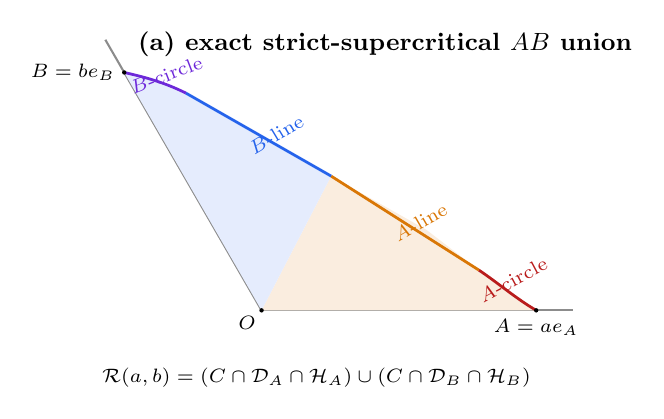
\begin{tikzpicture}[x=1.55cm,y=1.55cm,>=Latex]
  \node[panellabel,anchor=west] at (-1.05,2.18)
    {(a) exact strict-supercritical $AB$ union};
  \coordinate (O) at (0,0);
  \coordinate (A) at (2.25,0);
  \coordinate (B) at (-1.125,1.949);
  \coordinate (P1) at (1.78,.33);
  \coordinate (Qm) at (1.35,.66);
  \coordinate (Q0) at (.57,1.10);
  \coordinate (Qp) at (-.08,1.46);
  \coordinate (P4) at (-.62,1.78);
  \draw[black!45,line width=.75pt] (O)--(2.55,0);
  \draw[black!45,line width=.75pt] (O)--(-1.28,2.217);

  \fill[VertexOrange!13]
    (O)--(A).. controls (2.08,.10) and (1.93,.23)..(P1)--(Qm)--(Q0)--cycle;
  \fill[CenterBlue!12]
    (O)--(Q0)--(Qp)--(P4).. controls (-.82,1.88) and (-1.00,1.92)..(B)--cycle;

  \draw[DemandRed,line width=1pt]
    (A).. controls (2.08,.10) and (1.93,.23)..(P1);
  \draw[VertexOrange,line width=1pt] (P1)--(Q0);
  \draw[CenterBlue,line width=1pt] (Q0)--(P4);
  \draw[GapPurple,line width=1pt]
    (P4).. controls (-.82,1.88) and (-1.00,1.92)..(B);

  \fill (A) circle (.018) node[below=2pt,figlabel] {$A=ae_A$};
  \fill (B) circle (.018) node[left=2pt,figlabel] {$B=be_B$};
  \fill (O) circle (.018) node[below left=1pt,figlabel] {$O$};
  \node[figlabel,text=DemandRed,rotate=28] at (2.06,.25) {$A$-circle};
  \node[figlabel,text=VertexOrange,rotate=30] at (1.30,.72) {$A$-line};
  \node[figlabel,text=CenterBlue,rotate=31] at (.12,1.44) {$B$-line};
  \node[figlabel,text=GapPurple,rotate=21] at (-.78,1.93) {$B$-circle};
  \node[figlabel,align=center] at (.45,-.55)
    {$\mathcal R(a,b)=(C\cap\mathcal D_A\cap\mathcal H_A)
      \cup(C\cap\mathcal D_B\cap\mathcal H_B)$};
\end{tikzpicture}%
}
\end{minipage}\hfill
\begin{minipage}[t]{.48\linewidth}
\centering
\resizebox{.96\linewidth}{!}{%
\begin{tikzpicture}[x=1.55cm,y=1.55cm,>=Latex]
  \node[panellabel,anchor=west] at (-1.05,2.18)
    {(b) the three asymmetric frontier witnesses};
  \coordinate (O) at (0,0);
  \coordinate (A) at (2.25,0);
  \coordinate (B) at (-1.125,1.949);
  \coordinate (P1) at (1.78,.33);
  \coordinate (Qm) at (1.35,.66);
  \coordinate (Q0) at (.57,1.10);
  \coordinate (Qp) at (-.08,1.46);
  \coordinate (P4) at (-.62,1.78);
  \draw[black!45,line width=.75pt] (O)--(2.55,0);
  \draw[black!45,line width=.75pt] (O)--(-1.28,2.217);
  \draw[black!55,line width=.75pt]
    (A).. controls (2.08,.10) and (1.93,.23)..(P1)--(Q0)--(P4)
    .. controls (-.82,1.88) and (-1.00,1.92)..(B);
  \fill[DemandRed] (Qm) circle (.035) node[below right=2pt,figlabel] {$Q_-$};
  \fill[DemandRed] (Q0) circle (.035) node[right=2pt,figlabel] {$Q_0$};
  \fill[DemandRed] (Qp) circle (.035) node[above right=2pt,figlabel] {$Q_+$};

  \draw[black!35,dashed] (Qm) circle (.76);
  \draw[black!35,dashed] (Qp) circle (.76);
  \draw[flow] (Qm)--($(Qm)!1.42!(O)$);
  \draw[flow] (Q0)--($(Q0)!1.42!(O)$);
  \draw[flow] (Qp)--($(Qp)!1.42!(O)$);
  \node[figlabel,atlasbox,align=left,anchor=west] at (.80,1.57)
    {frontier excludes the actual supercritical role;\\
     moving unit-circle signs exclude the two adjacent roles;\\
     vertex distances exclude the three nonlocal roles};
  \node[figlabel,align=center] at (.45,-.55)
    {$Q_-,Q_0,Q_+\in\operatorname{int}(H)
      \setminus\bigcup_{i=0}^{5}U_i$};
\end{tikzpicture}%
}
\end{minipage}
\caption{The strict-supercritical $AB$ frontier and the three asymmetric
witnesses.  The source-conditioned union has, in counterclockwise order, an
$A$-circle arc, an $A$-line segment, a $B$-line segment, and a $B$-circle
arc.  The points $Q_-,Q_0,Q_+$ are selected on this exact frontier and are
then excluded from the six actual V roles by frontier, moving-circle, and
vertex-distance arguments.  The drawing is schematic; the labelled frontier
order and witness roles are exact.}
\label{fig:strict-ab-frontier-witnesses}
\end{figure}


\begin{proof}
The identities
\[
 4\rho-3(a+b)^2=(a-b)^2,
 \qquad
 (a+b)^2D^2-(a-b)^2=4\rho((a+b)^2-1)
\]
give $0<D<1$ and positivity of the four coefficients.

We apply the caliper criterion of \zcref{thm:cert-caliper}.  For a
point $x=(u,v)$ in the relative interior of $C$ but outside
$\triangle OAB$, the four hull vertices occur in the order $O,B,x,A$.
The two cone-axis hull edges cannot certify a unit triangle: their support
sums, divided by $h$, are respectively
\[
 \max\{a,u\}+\max\{b,v-u\},\qquad
 \max\{b,v\}+\max\{a,u-v\},
\]
and are at least $a+b>1$.  It remains to test the $Ax$ and $Bx$ calipers.

For the $Ax$ caliper put $p=u-a$ and
$r^2=p^2+v^2-pv$.  Exact evaluation of the three supports gives
\begin{equation}
 \frac{G_A}{h}=
 \frac{\max\{r^2,-ap+(a+b)v\}+N_A}{r},
 \quad
 N_A=\begin{cases}
 0,&p\le0,\\
 ap,&0\le p\le v,\\
 (a+b)p-bv,&p\ge v.
 \end{cases}                                      \label{eq:Ax-caliper}
\end{equation}
No support label is omitted in these three sectors.  If $p\le0$,
$G_A\le h$ is equivalent to
\[
 r\le1,\qquad -ap+(a+b)v\le r.
\]
The second inequality is the half-plane condition in
\eqref{eq:strict-ab-identity}, because
\[
 r^2-(-ap+(a+b)v)^2
 =\frac{(cp+dv)(c'p+d'v)}{4\rho},
\]
where
\[
 c=a+2b-aD,\quad d=a-b+(a+b)D,
 \quad c'=a+2b+aD,\quad d'=a-b-(a+b)D,
\]
and $c,c',d>0>d'$.  Thus the low sector is exactly
$\mathcal D_A\cap\mathcal H_A$.  In the middle sector $0<p\le v$ one has
$r\le v$, whereas the numerator in \eqref{eq:Ax-caliper} is at least
$(a+b)v>r$, so no fit is possible.

In the high sector $p\ge v$, the inequalities $G_A\le h$ imply
\begin{equation}
 r^2+(a+b)p-bv\le r,\qquad bp+av\le r.          \label{eq:Ax-high}
\end{equation}
Write $x-A=ry(\theta)$, $0\le\theta\le60^\circ$, with cone coordinates
\[
 y(\theta)=te_A+we_B,\quad
 t=\frac2{\sqrt3}\cos(\theta-30^\circ),\quad
 w=\frac2{\sqrt3}\sin\theta.
\]
Then \eqref{eq:Ax-high} gives
\[
 r\le f(\theta)=1-(a+b)t+bw,\qquad S(\theta)=bt+aw\le1.
\]
Let $n_B$ be the unit vector with dual coordinates $(\gamma,\delta)$.
The identities
\[
 b\gamma+(a+b)\delta=h,\quad
 (a+b)\gamma+a\delta=\frac h2(1+D),\quad
 b\delta-a\gamma=\frac h2(1-D)
\]
show that the unique angle $\theta_B$ of this normal satisfies
$S(\theta_B)=1$ and $f(\theta_B)=(1-D)/2$.  The function $S$ has at most
one critical point, a maximum, so $S(\theta)\le1$ implies
$\theta\le\theta_B$.  On the feasible part $f,f'\ge0$; hence
$f(\theta)\cos(\theta_B-\theta)$ is increasing.  Consequently
\[
 \langle n_B,x-B\rangle
 \le a\gamma-b\delta+\frac h2(1-D)=0.
\]
The diameter bound also gives $\lVert x-B\rVert\le1$.  Thus every high
sector fit belongs to $\mathcal D_B\cap\mathcal H_B$.  Reflection exchanges
$a,u$ with $b,v$ and supplies the corresponding result for the $Bx$
caliper.  This proves \eqref{eq:strict-ab-identity} in the cone interior;
the axes follow by taking limits, since both sides are closed.

For completeness, the line--circle junctions are obtained by solving the
two displayed line and circle equations.  The line normals satisfy
\[
 \alpha^2+\alpha\beta+\beta^2=h^2,\qquad
 \gamma^2+\gamma\delta+\delta^2=h^2,
\]
and the line determinant is
\[
 \alpha\delta-\gamma\beta
 =\frac{3(1-D)(D+3)}{16\rho}>0.
\]
The successive cone slopes are
\[
 +\infty,\quad \frac2{1-D},\quad
 \frac{a(1-D)+2b}{2a+b(1-D)},\quad
 \frac{1-D}{2},\quad0;
\]
the two middle comparisons reduce to
$a(4-(1-D)^2)>0$ and $b(4-(1-D)^2)>0$.  This proves the asserted four-piece
order.
\end{proof}

\paragraph{Body consequence.}
This supplies the exact feasible-union and maximal-line-piece evaluation used
to define $\ell_-,\ell_+$ and $Q_0$ in the body, and is cited there as
\zcref{thm:strict-ab-union}.

\subsection{Handoff and nine-point frontier-forcing module}

\paragraph{Exact interface.}
The body interface is the exact chain and parameter domain in
\zcref{eq:reader-extreme-chain,eq:reader-ab-parameters,eq:reader-ab-domain},
the forced disk in \zcref{eq:reader-forced-disk}, the three frontier points
in \zcref{eq:reader-forced-asymmetric}, and the witness set in
\zcref{eq:reader-witness-set}.

\paragraph{Variables and feasible set.}
Assume $N_{\mathrm{gap}}=0$, $N_+=1$, and $(d,t)=(0,0)$; rotate the unique
supercritical role to index~$4$ and use the strict handoffs $\xi_i$ selected
in the body.  The feasible parameter pair is the strict component
$0<a,b<1$, $a+b>1$, $a^2+ab+b^2<1$ determined below.

\paragraph{Objective.}
Determine the common radial envelope and the two line--circle roots, then
prove that the resulting six radial points and three asymmetric frontier
points are excluded from every V triangle.

\paragraph{Exact result.}
The exact outputs are supplied by
\zcref{lem:ab-extreme-jump,lem:symmetric-core-witness,lem:fixed-line-signs,lem:asymmetric-core-witness}:
they give the strict endpoint inequalities, the forced centered disk, the
unique frontier roots, and $K_{\rm wit}(a,b)\subset U_C$.

\paragraph{Solution.}

\subsubsection*{Handoff stage}

\begin{lemma}[Exact-one handoff chain]
\label{lem:ab-extreme-jump}
Assume the six V triangles cover $\partial H$ and exactly one actual V triangle is
supercritical.  Rotate its index to $4$.  The strict handoffs supplied by
\zcref{prop:strict-handoffs} satisfy
\[
 \xi_3<\xi_2<\xi_1<\xi_0<\xi_5<\xi_4.                       \label{eq:extreme-chain}
\]
With
\[
 a=1-\xi_3,\qquad b=\xi_4,\qquad p=1-b,\qquad q=1-a,
\]
one has
\begin{equation}
 \begin{gathered}
 0<a,b<1,
 \qquad a=a_4<A_4,
 \qquad b=b_4<B_4,\\
 a+b>1,
 \qquad a^2+ab+b^2<1,
 \end{gathered}
 \label{eq:ab-strict-domain}
\end{equation}
and every selected V triangle obeys
\[
 a_i\ge p,\qquad b_i\ge q.
\]
\end{lemma}

\begin{proof}
Every selected V triangle other than $4$ is strictly nonsupercritical, so
$\xi_i<\xi_{i-1}$ for $i\ne4$, which is precisely
\eqref{eq:extreme-chain}.  In particular $\xi_3$ is the global minimum and
$\xi_4$ the global maximum.  Strictness of the selected handoffs gives
$a=1-\xi_3=a_4<A_4$ and $b=\xi_4=b_4<B_4$.  The two anchors of V
triangle $4$ lie in its open triangle;
their mutual squared distance is $a^2+ab+b^2$, strictly below the diameter
squared of the closed unit triangle.  This proves \eqref{eq:ab-strict-domain}.
Finally every $\xi_j\in[\xi_3,\xi_4]$, so
$1-\xi_{i-1}\ge1-\xi_4=p$ and $\xi_i\ge \xi_3=q$.
\end{proof}

\subsubsection*{Radial stage}

Put $h=\sqrt3/2$ and
\[
 s=p+q,\qquad m=\min(p,q),\qquad M=\max(p,q),
 \qquad \chi=s^4-s^2+pq.
\]
The strict domain \eqref{eq:ab-strict-domain} gives
\begin{equation}
 pq>(1-s)(2-s),\qquad m>1-s,\qquad s>1-m.         \label{eq:pq-domain}
\end{equation}
Let $c_*=c_{\max}(p,q)$ be the exact radial envelope of
\zcref{prop:exact-admissible-set}.  On the present subcritical
domain, equation \eqref{eq:radial-envelope} becomes
\begin{equation}
 c_*=\begin{cases}
 C_L(m),&\chi\le0,\\[1mm]
 \displaystyle\frac{2M}{1+\sqrt{4s^2-3}},&\chi>0,
 \end{cases}                                    \label{eq:core-cstar}
\end{equation}
where $C_L(m)$ is the unique root in $[\sqrt3/2,1]$ of
\[
 z^4-z^2+mz-m^2=0.
\]
At $\chi=0$ the two expressions agree and equal $s$.

\begin{lemma}[Direct radial forcing]
\label{lem:symmetric-core-witness}
One has
\begin{equation}
 0<c_*<1,\qquad c_*>1-m.                         \label{eq:cstar-bounds}
\end{equation}
Assume that every $U_i$ is $\Vdzero$ and that
$U_C,U_0,\ldots,U_5$ cover $H$.  Then, for every $i$,
\[
 P_i^{\mathrm{rad}}=(1-c_*)V_i\in U_C.
\]
Consequently
\begin{equation}
 \mathbb B(0,r_*)=\{x:\lVert x\rVert\le r_*\}
 \subseteq\conv\{P_0^{\mathrm{rad}},\ldots,P_5^{\mathrm{rad}}\}
 \subset U_C,
 \qquad r_*=h(1-c_*).                           \label{eq:forced-disk}
\end{equation}
\end{lemma}

\begin{proof}
On the $C_L$ branch, $C_L(m)<1$ because the defining polynomial is positive
at $1$; if $s<\sqrt3/2$, then $c_*\ge\sqrt3/2>s>1-m$, while if
$s\ge\sqrt3/2$ its value at $s$ is $\chi\le0$, so $c_*\ge s>1-m$.
On the other branch put $E=\sqrt{4s^2-3}$.  The selector gives
$sE>M-m$, whence $c_*<s<1$.  Moreover, with
\[
 A_*=\frac{2M}{1-m}-1,
\]
one has
\[
 A_*^2-E^2=
 \frac{4(1-s)\{(1-m)(1-2m)+m(2-m)(1-s)\}}{(1-m)^2}>0.
\]
Thus $A_*>E$ and $c_*>1-m$.  This proves
\eqref{eq:cstar-bounds}.

Fix $i$.  If $P_i^{\mathrm{rad}}\in U_i$, openness supplies $\varepsilon>0$ with
$c_*+\varepsilon<1$ such that
$(1-c_*-\varepsilon)V_i\in U_i$.  The same triangle contains its two selected
handoff anchors.  Since their incoming and forward-reach lower bounds dominate $p$ and
$q$, convexity and passage to the closure give a closed unit triangle
realizing $(p,q,c_*+\varepsilon)$.  This contradicts the definition of
$c_*=c_{\max}(p,q)$.  Hence $P_i^{\mathrm{rad}}\notin U_i$.

If $P_i^{\mathrm{rad}}$ belonged to $U_{i-1}$ or $U_{i+1}$, a small plane
ball inside that
open triangle would meet $r_i$ in a positive-length
interval.  This contradicts the $\Vdzero$ definition.  For the remaining
triangles put $r=1-c_*>0$.  Directly,
\[
 \lVert rV_i-V_{i\pm2}\rVert^2=1+r+r^2>1,
 \qquad
 \lVert rV_i-V_{i+3}\rVert=1+r>1.
\]
Since $V_j\in U_j$ and two points of an open unit triangle are at distance
strictly below $1$, these inequalities exclude $P_i^{\mathrm{rad}}$ from the
other three V triangles.  Thus no V triangle contains
$P_i^{\mathrm{rad}}$.  The point lies in
$\interior(H)$ by \eqref{eq:cstar-bounds}, so the assumed cover forces
$P_i^{\mathrm{rad}}\in U_C$.

The six points $P_i^{\mathrm{rad}}$ form a regular hexagon of circumradius
$1-c_*$.  Their
convex hull contains its centered incircle of radius $h(1-c_*)$, and convexity
of $U_C$ gives \eqref{eq:forced-disk}.
\end{proof}

\subsubsection*{Asymmetric frontier stage}

We next define the three asymmetric witnesses.  At $V_4$ use local
coordinates
\[
 \Phi(u,v):=V_4+u(V_5-V_4)+v(V_3-V_4),\qquad
 \mathsf q(u,v)=u^2+v^2-uv.
\]
In this chart the two public adjacent-handoff circles have centers
\[
 \begin{aligned}
 X_2(b)&=\Phi(E_-),& E_-&=(1-b,2-b),\\
 X_5(1-a)&=\Phi(E_+),& E_+&=(2-a,1-a),
 \end{aligned}
\]
and hence
\[
 \mathcal C_-=\partial\mathbb B(\Phi(E_-),1),
 \qquad
 \mathcal C_+=\partial\mathbb B(\Phi(E_+),1).
\]
The forward-reach lower bound is $b$ and the backward-reach lower bound is $a$.  Accordingly,
set
\begin{align*}
 \alpha&=\frac{h(b+2a-bD)}{2\rho},&
 \beta&=\frac{h(b-a+(a+b)D)}{2\rho},\\
 \gamma&=\frac{h(-b+a+(a+b)D)}{2\rho},&
 \delta&=\frac{h(2b+a-aD)}{2\rho},
\end{align*}
where now $\rho=a^2+ab+b^2$ and $D=\sqrt{4\rho-3}$.  The two line pieces of
\zcref{thm:strict-ab-union} are
\[
 L_-(\lambda)=(b-\beta\lambda,\alpha\lambda),\qquad
 L_+(\mu)=(\delta\mu,a-\gamma\mu).
\]
They meet at $\lambda_* =\mu_*=8h\rho/(3(D+3))$ in
\begin{equation}
 J=\left(\frac{2b+a-aD}{D+3},
          \frac{b+2a-bD}{D+3}\right).           \label{eq:line-junction}
\end{equation}
Thus the two public line pieces have the coordinate evaluations
\[
 \ell_-=\{\Phi(L_-(\lambda)):\lambda_*\le\lambda\le h^{-1}\},
 \qquad
 \ell_+=\{\Phi(L_+(\mu)):\mu_*\le\mu\le h^{-1}\}.
\]
The actual adjacent handoffs have local centers
\[
 Z_5(t)=(1+t,t),\qquad 1-a\le t\le b,
 \quad\text{and}\quad
 Z_3(y)=(y,1+y),\qquad 1-b\le y\le a.
\]
The restrictions of the two unit-circle equations are
\begin{align}
 g_-(\lambda)&=\frac34\lambda^2
 -3(\alpha+b\beta)\lambda+3b^2-3b+2,\notag\\
 g_+(\mu)&=\frac34\mu^2
 -3(\delta+a\gamma)\mu+3a^2-3a+2.              \label{eq:witness-quadratics}
\end{align}
Let $\lambda_-$ and $\mu_+$ be their first roots; explicitly,
\begin{align*}
 \lambda_-&=2(\alpha+b\beta)
 -\frac23\sqrt{9(\alpha+b\beta)^2-9b^2+9b-6},\\
 \mu_+&=2(\delta+a\gamma)
 -\frac23\sqrt{9(\delta+a\gamma)^2-9a^2+9a-6}.
\end{align*}

\begin{lemma}[Moving adjacent-triangle signs]
\label{lem:fixed-line-signs}
Throughout \eqref{eq:ab-strict-domain},
\begin{equation}
 \lambda_*<\lambda_-<h^{-1},\qquad
 \mu_*<\mu_+<h^{-1}.                            \label{eq:first-root-order}
\end{equation}
Moreover $J_u,J_v<1/2$.  The point $L_+(\mu_+)$ satisfies
\[
 (L_+(\mu_+))_u+(L_+(\mu_+))_v<3-2a,
\]
and the reflected bound holds for $L_-(\lambda_-)$.  Writing
$F(P,t)=\mathsf q(P-Z_5(t))-1$, one has, for every $t\in[1-a,b]$,
\begin{equation}
 F(L_+(\mu_+),t)\ge0,\qquad F(J,t)>0,\qquad
 F(L_-(\lambda_-),t)>0.                           \label{eq:moving-right-signs}
\end{equation}
Under the reflection
$(u,v,a,b)\leftrightarrow(v,u,b,a)$, the analogous signs hold for every
$y\in[1-b,a]$: the first-root point $L_-(\lambda_-)$ has nonnegative sign
against $Z_3(y)$, and the other two witnesses have strictly positive sign.
\end{lemma}

\begin{proof}
Put
\[
 U=a+b-1,\qquad z=a-b,\qquad
 D^2=z^2+6U+3U^2.
\]
Then $0<U<1/6$ and $z^2<\Omega:=1-6U-3U^2$.  We give the
fixed-line calculation for the circle centered at
$E_+=(2-a,1-a)$; reflection gives the calculation for $E_-$.  Put
\[
 F(P,t)=\mathsf q(P-(1+t,t))-1,\qquad t_0=1-a,
\]
so this circle is $F(P,t_0)=0$.  At the junction, exact expansion gives
\[
 (D+3)^2F(J,t_0)=3D(z^2+Uz+1-3U)+P_J,
\]
where
\[
 P_J=z^4+5z^2+6Uz^2+3U^2z^2+9Uz+3U+15U^2>0;
\]
indeed $z^2+Uz+1-3U\ge1-3U-U^2/4>0$, and
$5z^2+9Uz+15U^2$ is positive definite.  Thus $F(J,t_0)>0$.
Also
\[
 J_u+J_v=\frac{(1+U)(3-D)}{3+D}<1.
\]
Indeed this inequality is $3U<D(2+U)$, which follows from
$D^2\ge3U(2+U)$ and $(2+U)^3>3U$.  Since
\[
 \frac{\partial F}{\partial t}(P,t)=1+2t-P_u-P_v,
\]
$F(J,t)$ is strictly increasing for $t\ge0$, and therefore is positive
throughout $[1-a,b]$.

On the opposite line $L_-$, the derivative at the junction, after
multiplication by a positive factor, has at $t=1-a$ the numerator
\[
 N_0=D(9+3z^2+6Uz-9U^2)+P_0,
\]
where
\[
\begin{aligned}
 P_0={}&18U^3+6U^2z^2+63U^2+18Uz^2+18Uz+54U\\
      &+2z^4+9z^2+9.
\end{aligned}
\]
The coefficient of $D$ is at least $9-6U-9U^2>0$, while
$P_0\ge9+54U-18U>0$.  Hence $N_0>0$.  At the other endpoint $t=b$, the
corresponding numerator is
\[
 N_1=D(9+3z^2+6U-3U^2)+P_1,
\]
where
\[
\begin{aligned}
 P_1={}&9U^4-3U^3z+45U^3+9U^2z^2-6U^2z+72U^2\\
      &-Uz^3+21Uz^2+9Uz+45U+2z^4+9z^2+9.
\end{aligned}
\]
Its $D$-coefficient is positive and, using $|z|<1$,
\[
 P_1\ge9+45U-9U-U-6U^2-3U^3>0.
\]
The junction derivative is affine in $t$, so it is positive throughout
$[1-a,b]$.  Since the restriction of $F$ to $L_-$ is a convex quadratic,
is positive at the junction, and is increasing there, it has no intersection
on the opposite line side for any actual adjacent handoff.

On the correct line $L_+$, the value at its outer endpoint $h^{-1}$ has,
after multiplication by a positive factor, numerator
\[
 A_*=P_2-4DU(1+U+z),
\]
where
\[
\begin{aligned}
 P_2={}&3U^4+6U^3z+6U^3+4U^2z^2+12U^2z+12U^2\\
      &+2Uz^3+6Uz^2+2Uz+6U+z^4+2z^2-3.
\end{aligned}
\]
For fixed $U$, replace the odd powers of $z$ by $x=|z|$.  The resulting
polynomial $P_2^+(U,x)$ satisfies
\[
 \partial_xP_2^+
 =2(3U^3+4U^2x+6U^2+3Ux^2+6Ux+U+2x^3+2x)>0,
\]
and therefore its supremum for $z^2<\Omega$ occurs at $x=\sqrt\Omega$.
There
\[
 P_2^+(U,\sqrt\Omega)=4U(U+\sqrt\Omega-3)<0.
\]
As $1+U+z=2a>0$, this gives $A_*<0$.  The positive junction value and
negative endpoint value force the first root strictly between them, proving
the $L_+$ half of \eqref{eq:first-root-order}; reflection proves the other
half.

For the coordinate bounds, the exact identities
\[
 D^2-(3U-z)^2=6U(1+z-U),\qquad
 D^2-(3U+z)^2=6U(1-z-U)
\]
give $J_u,J_v<1/2$.  It remains to control the coordinate sum along $L_+$.
For $E=L_+(h^{-1})$, the sign of $3-2a-E_u-E_v$ is the sign of
\[
 D(6U+2z+6)+B(U,z),
\]
where
\[
\begin{aligned}
 B(U,z)={}&-9U^3-9U^2z-9U^2-3Uz^2-18Uz+3U\\
          &-3z^3+3z^2-3z+3.
\end{aligned}
\]
Here
\[
 B_z=-3(3z^2+2Uz+6U-2z+3U^2+1)<0,
\]
because the quadratic in parentheses has discriminant
$-32U^2-80U-8<0$.  Hence its minimum on $z^2<\Omega$ is at
$z=\sqrt\Omega$, where
$B(U,\sqrt\Omega)=6(1-3U-\sqrt\Omega)>0$ because
$(1-3U)^2-\Omega=12U^2$.  Thus $E_u+E_v<3-2a$.
Also $J_u+J_v<1<3-2a$, and the coordinate sum is affine on the
line segment, so the same strict bound holds at the first root.  Now
\[
 \frac{\partial F}{\partial t}(P,t)=1+2t-P_u-P_v.
\]
Since $F(L_+(\mu_+),1-a)=0$, the coordinate-sum bound makes its $t$-derivative
strictly positive for $t\ge1-a$.  Together with the no-opposite-line result,
this proves \eqref{eq:moving-right-signs}.  Reflection gives both the bound on
$L_-$ and the complete $Z_3(y)$ statement.
\end{proof}

Define the local and global witnesses by
\begin{equation}
 Q_-^{\rm loc}=L_-(\lambda_-),\qquad
 Q_0^{\rm loc}=J,\qquad
 Q_+^{\rm loc}=L_+(\mu_+),                       \label{eq:asym-witnesses}
\end{equation}
and
\[
 Q_-:=\Phi(Q_-^{\rm loc}),
 \qquad Q_0:=\Phi(Q_0^{\rm loc}),
 \qquad Q_+:=\Phi(Q_+^{\rm loc}).
\]
Thus $J$ is the unique meeting point of the two maximal line pieces, and the
first-root inequalities in \zcref{lem:fixed-line-signs} give exactly
\[
 \{Q_0\}=\ell_-\cap\ell_+,
 \qquad
 \{Q_-\}=\ell_-\cap\mathcal C_-,
 \qquad
 \{Q_+\}=\ell_+\cap\mathcal C_+.
\]

\begin{lemma}[Direct asymmetric forcing]
\label{lem:asymmetric-core-witness}
Assume that $U_C,U_0,\ldots,U_5$ cover $H$.  Then
\[
 Q_-,Q_0,Q_+
 \in\interior(H)\setminus\bigcup_{i=0}^5U_i,
\]
and consequently all three witnesses belong to $U_C$.
\end{lemma}

\begin{proof}
The root order and positivity of the line coordinates give
$0<u,v<1$ for all three points.  Each belongs to the local representation
of $\mathcal R_{AB}(a,b)$ obtained from \zcref{thm:strict-ab-union} by
interchanging the two cone coordinates, and hence
lies in a closed unit triangle containing $V_4$, so
$\mathsf q(u,v)\le1$; hence
$|u-v|<1$ and all three points lie in $\interior(H)$.

The closure of $U_4$ is one of the triangles represented by
$\mathcal R_{AB}(a,b)$, since it contains $V_4,X_3,X_4$.  All three witnesses lie
on its exact non-axis frontier.  If one belonged to the open triangle $U_4$,
a sufficiently small plane ball about it would lie both in $U_4$ and in the
interior of the corner cone, making the witness an interior point of
$\mathcal R_{AB}(a,b)$.  This contradiction excludes $U_4$.

For the triangles $U_0,U_1,U_2$, their contained vertices have local coordinates
\[
 \begin{array}{c|ccc}
 i&0&1&2\\ \hline
 V_i&(2,1)&(2,2)&(1,2).
 \end{array}
\]
For $P=(u,v)$,
\[
 \lVert P-(2,1)\rVert^2-1=\mathsf q(u,v)+2-3u,
 \quad
 \lVert P-(1,2)\rVert^2-1=\mathsf q(u,v)+2-3v.
\]
The inequalities $J_u,J_v<1/2$ and the line order give distance greater than
one from $V_0$ for $Q_-,Q_0$ and from $V_2$ for $Q_0,Q_+$.  For the remaining
pair, the first-root circle and the sum bound in
\zcref{lem:fixed-line-signs} give
\[
 \lVert Q_+-V_0\rVert^2-1
 =a(3-a-(Q_+)_u-(Q_+)_v)>a^2,
\]
and, by reflection, $\lVert Q_--V_2\rVert^2-1>b^2$.  All three points are
farther than one from $V_1=(2,2)$, because writing $u=1-\xi$, $v=1-\eta$
gives
\[
 \lVert P-V_1\rVert^2
 =1+\xi+\eta+\xi^2+\eta^2-\xi\eta>1.
\]
Since two points in one open unit equilateral triangle have distance strictly
less than one, these inequalities exclude $U_0,U_1,U_2$.

The actual handoff $X_5=Z_5(\xi_5)$ belongs to $U_5$, and
$1-a<\xi_5<b$ by \eqref{eq:extreme-chain}.  The three signs in
\eqref{eq:moving-right-signs} therefore put every witness at distance at
least one from $X_5$, excluding $U_5$.  Similarly, if $y=1-\xi_2$, then
$1-b<y<a$, $X_2=Z_3(y)\in U_3$, and the reflected signs exclude $U_3$.
Thus no V triangle contains any witness.  The assumed cover now forces all
three interior witnesses into $U_C$.
\end{proof}

The nine directly forced points are
$P_0^{\mathrm{rad}},\ldots,P_5^{\mathrm{rad}},Q_-,Q_0,Q_+$.  Under a
putative cover, \zcref{lem:symmetric-core-witness,lem:asymmetric-core-witness}
therefore force the compact set
\begin{equation}
 K_{\rm wit}(a,b)=
 \mathbb B(0,r_*)\cup\{Q_-,Q_0,Q_+\}
 \subset U_C.                                    \label{eq:forced-witness-set}
\end{equation}

\paragraph{Body consequence.}
This is the full calculation supplying the body containments
\zcref{eq:reader-forced-disk,eq:reader-forced-asymmetric,eq:reader-witness-set}.

\subsection{Newton reduction and four-overlap module}

\paragraph{Exact interface.}
Retain the public $K_{\rm wit}(a,b)$ from
\zcref{eq:reader-witness-set} and the exact support cap
\[
 \operatorname{Cap}(X,r)
 =\{n\in\mathbb S^1:\langle X,n\rangle+r\ge h\}.
\]

\paragraph{Variables and feasible set.}
Work on the strict $AB$ domain in \eqref{eq:ab-strict-domain} and its
nontrivial sheet $c_*>2/3$.  The Newton parameters are taken on the open
segments from the line junction $Q_0$ to the first circle roots $Q_-$ and
$Q_+$.

\paragraph{Objective.}
Replace the two independent first-root radicals by rational inner points and
verify the ray order, radius bounds, and four consecutive support-cap
intersections needed for the cyclic enclosure argument.

\paragraph{Exact result.}
The Newton containment is
\zcref{lem:technical-newton-reduction,eq:reader-newton-reduction}, and the
complete four-overlap conclusion is
\zcref{prop:technical-four-overlaps}.

\paragraph{Solution.}

For the nontrivial regime $c_*>2/3$, we first remove the square radicals in
the first-root witnesses.  Normalize
$\bar\alpha=\alpha/h$, and similarly for the other three coefficients, and
put
\[
 \xi=\lambda/h,\quad \zeta=\mu/h,\quad
 \xi_*=\zeta_*=\frac{8\rho}{3(D+3)}.
\]
Let $g_-,g_+$ be the rescaled forms of
\eqref{eq:witness-quadratics}, and take one Newton step at the junction:
\[
 \widehat\xi_-=\xi_*-\frac{g_-(\xi_*)}{g_-'(\xi_*)},\qquad
 \widehat\zeta_+=\zeta_*-\frac{g_+(\zeta_*)}{g_+'(\zeta_*)}.
\]
Define, in local coordinates,
\begin{align*}
 P_-&=\left(b-\frac34\bar\beta\widehat\xi_-,
          \frac34\bar\alpha\widehat\xi_-\right),\\
 P_0&=J,\\
 P_+&=\left(\frac34\bar\delta\widehat\zeta_+,
          a-\frac34\bar\gamma\widehat\zeta_+\right),
\end{align*}
and convert them to global vectors.

\begin{lemma}[Newton inner reduction]
\label{lem:technical-newton-reduction}
The points above have coordinates rational in $a,b,D$ and satisfy
\[
 P_-\in(Q_0,Q_-),\qquad P_0=Q_0,\qquad P_+\in(Q_0,Q_+).
\]
Consequently
\[
 \widehat K=\conv\bigl(\mathbb B(0,r_*)\cup\{P_-,P_0,P_+\}\bigr),
\]
and one has
\begin{equation}
 \widehat K\subseteq\conv(K_{\rm wit}),
 \qquad
 \Lambda(K_{\rm wit})\ge\Lambda(\widehat K).
 \label{eq:reader-newton-reduction}
\end{equation}
\end{lemma}

\begin{proof}
Each quadratic $g_-,g_+$ is strictly convex, positive, and decreasing at
the junction.  Its tangent zero therefore lies strictly between the
junction and its first root.  This gives the two open-segment inclusions.
All displayed coefficients and Newton quotients are rational in $a,b,D$,
and convexity gives the asserted containment.
\end{proof}

Put
\[
 P_*:=P_++\mathsf R P_-.
\]
For a disk $\mathbb B(X,r)$ let
\[
 \operatorname{Cap}(X,r)
 :=\{n\in\mathbb S^1:\langle X,n\rangle+r\ge h\}.
\]


\subsubsection*{Ray order and overlap verification}

\begin{proposition}[Technical four-overlap verification]
\label{prop:technical-four-overlaps}
Assume \eqref{eq:ab-strict-domain} and $c_*>2/3$.  Then
\[
 \lVert P_-\rVert,\lVert P_+\rVert>r_*,
\]
the rays $P_-,P_0,P_+,P_*,\mathsf R P_-$ occur in that cyclic order, and the
four consecutive
cap pairs
\[
 \operatorname{Cap}(P_-,2r_*)
 \leftrightarrow\operatorname{Cap}(P_0,2r_*)
 \leftrightarrow\operatorname{Cap}(P_+,2r_*)
 \leftrightarrow\operatorname{Cap}(P_*,r_*)
 \leftrightarrow\operatorname{Cap}(\mathsf R P_-,2r_*)
\]
overlap across their intervening short sectors.
\end{proposition}

\begin{proof}

Put $\tau=h-2r_*=h(2c_*-1)$.  The rays of
\begin{equation}
 P_-,\ P_0,\ P_+,\ P_*,\ \mathsf R P_-          \label{eq:cap-ray-order}
\end{equation}
occur in this cyclic order from $P_-$ to $\mathsf R P_-$.  Indeed the two
line distances
give
\[
 \frac{\operatorname{cross}(P_-,P_0)}{\lVert P_0-P_-\rVert}
 =\alpha(1-b)+\beta>0,
 \quad
 \frac{\operatorname{cross}(P_0,P_+)}{\lVert P_+-P_0\rVert}
 =\gamma+\delta(1-a)>0.
\]
If $P_-=(-X,-Y)$ and $P_+=(-P,-Q)$ in the centered cone basis, then
$0<X,Y,P,Q<1$, $X,Q>1/2$, and
\[
 \frac{\operatorname{cross}(P_+,\mathsf R P_-)}h
 =PX+(Q-P)Y>0.
\]
The last sign is immediate unless $Q<P$ and $X<Y$, in which case it is
larger than $Q-P/2>0$.  The ray of
$P_*=P_++\mathsf R P_-$ lies between those of $P_+$ and
$\mathsf R P_-$.  The same coordinates give
\begin{equation}
 \lVert P_-\rVert,\lVert P_+\rVert>h/2>r_*.
 \label{eq:outer-radii}
\end{equation}

For the two equal-radius overlaps it is enough to prove
\begin{equation}
 \frac{\operatorname{cross}(P_-,P_0)}{\lVert P_0-P_-\rVert}\ge\tau,
 \qquad
 \frac{\operatorname{cross}(P_0,P_+)}{\lVert P_+-P_0\rVert}\ge\tau.
 \label{eq:adjacent-overlaps}
\end{equation}
We now give the exact analytic verification.  By reflection take $a\le b$ and
set $m=1-b$, $M=1-a$, $U=a+b-1$, $s=m+M$, and $w=M-m$.  The smaller of the
two normalized left sides in \eqref{eq:adjacent-overlaps} is
\begin{equation}
 d=\frac{\mathcal A+U(2m-1)+D(\mathcal A+U)}{2\rho},
 \qquad \mathcal A=1-m+m^2.                      \label{eq:adjacent-d}
\end{equation}
On the $C_L$ sheet, write $F_L(z)=z^4-z^2+mz-m^2$.  This defining
polynomial evaluated at
$r=1-m/2+m^2/2$ is
\[
 F_L(r)=\frac{m^2(m-1)}{16}
 (m^5-3m^4+11m^3-17m^2+28m-12)>0.
\]
Indeed the polynomial in parentheses is increasing on $(0,1/2)$ and has
value $-33/32$ at $1/2$; its derivative is
$28-34m+m^2(5m^2-12m+33)>0$.  Since
$F_L(h)=-(m-h/2)^2\le0$ and the selected
root is unique, $2c_*-1\le\mathcal A$.  Put
\[
 X_0=\mathcal A+U,
 \qquad
 Y_0=2\rho\mathcal A-\mathcal A-U(2m-1).
\]
Then
\[
 d-\mathcal A=\frac{D(\mathcal A+U)-Y_0}{2\rho},
\]
and exact expansion gives
\[
\begin{aligned}
 Y_0={}&2(m^2-m+1)U^2+(2m^3-2m+3)U\\
      &+(m^2-m+1)(2m^2-2m+1)>0.
\end{aligned}
\]
Furthermore
\[
 D^2X_0^2-Y_0^2=4m\rho\Phi(U,m),
\]
where
\[
\begin{aligned}
 \Phi(U,m)={}&(1-m)(m^2-m+2)U^2\\
 &+(2-m^2)(m^2-m+1)U\\
 &-m(1-m)^2(m^2-m+1).
\end{aligned}
\]
In these variables
\[
 \chi=U^4-4U^3+5U^2-(m+2)U+m(1-m).
\]
Since $U^2(U^2-4U+5)>0$, the selector $\chi\le0$ implies
$U>m(1-m)/(m+2)$; $\Phi$ is increasing in $U$ and at that lower endpoint is
\[
 \frac{m^2(1-m)(m^4-2m^3+6m^2-6m+4)}{(m+2)^2}>0.
\]
The last quartic equals $(m^2-m)^2+5m^2-6m+4>0$.
Thus $d>\mathcal A\ge2c_*-1$.

On the other radial sheet let $E=\sqrt{4s^2-3}$.  Then
$0\le w<sE$ and $c_*=(s+w)/(1+E)$.  At fixed $U$, differentiation of
\eqref{eq:adjacent-d} can be checked without an implicit estimate.  Namely,
\[
 d=\frac{1+D}{2}-UB(D,w),\qquad
 B(D,w)=\frac{(1+U)(3+D)+w(1-D)}{D^2+3}.
\]
Here $D^2=w^2+6U+3U^2$, so $0\le D'=w/D\le1$, and
\[
 B_w=\frac{1-D}{D^2+3}\ge0.
\]
Writing $N=(1+U)(3+D)+w(1-D)$, direct differentiation gives
\[
 B_D=\frac{(1+U-w)(D^2+3)-2DN}{(D^2+3)^2}>-\frac{34}{27}.
\]
Indeed the first term in the numerator is positive, while
$1+U-w=2a>0$, $N<(7/6)4+1=17/3$, $D<1$, and $D^2+3\ge3$.  If $B_D<0$, then
$B_DD'\ge B_D$; otherwise $B_DD'\ge0$.  Hence
$B'=B_w+B_DD'>-34/27$, and $U<1/6$ yields
\[
 d'<\frac12+\frac16\frac{34}{27}=\frac{115}{162}<1,
\]
whereas
$(2c_*-1)'=2/(1+E)\ge1$.  Hence their difference decreases with $w$.
At the boundary $w=sE$, where $\chi=0$ and $c_*=s$, the preceding sheet
applies: this is an admissible point because $h<s<1$ and
$D^2=4s^4-12s+9<1$.  Indeed
$s^4-3s+2=(s-1)(s^3+s^2+s-2)<0$ on this interval; the second factor is
increasing and already equals $(7h-5)/4>0$ at $s=h$.  The preceding sheet gives
$d\ge2s-1$.  Therefore \eqref{eq:adjacent-overlaps} holds on both
sheets, and reflection supplies the other line.

It remains to check the two mixed overlaps.  The exact rational envelopes,
Gram reductions, and global positive-basis identities are recorded once in
\zcref{sec:strategy4-exact-certificate}.
\zcref{thm:paper-exact-mixed-certificate} gives precisely the overlaps for
$\mathbb B(P_+,2r_*)$ with $\mathbb B(P_*,r_*)$ and for
$\mathbb B(P_*,r_*)$ with $\mathbb B(\mathsf R P_-,2r_*)$.

Thus the four consecutive pairs of caps centered on the rays
\eqref{eq:cap-ray-order} overlap.
\end{proof}

\paragraph{Body consequence.}
These exact Newton and overlap data supply the nontrivial branch of the
support-arc solution below, and hence the body conclusion
\zcref{thm:reader-witness-enclosure}.

\subsection{Support-arc enclosure module}
\label{subsec:nine-point-conclusion}

\paragraph{Exact interface.}
The body supplies the compact witness
\[
 K_{\rm wit}(a,b)=\mathbb B(0,r_*)\cup\{Q_-,Q_0,Q_+\}
\]
in \zcref{eq:reader-witness-set}, together with the exact level-$h$ cap
\[
 \operatorname{Cap}(X,r)
 =\{n\in\mathbb S^1:\langle X,n\rangle+r\ge h\}.
\]

\paragraph{Variables and feasible set.}
The parameters satisfy $0<a,b<1$, $a+b>1$, and
$a^2+ab+b^2<1$.  The disk branch is split exactly at $c_*=2/3$; on the
strict branch $c_*>2/3$, use the Newton points and cap overlaps from the
preceding module.  All support directions range over the closed unit circle
$\mathbb S^1$.

\paragraph{Objective.}
Determine the enclosure gauge of $K_{\rm wit}(a,b)$ by proving the sharp
sufficient bound $\Lambda(K_{\rm wit}(a,b))\ge1$ on the entire feasible
domain.

\paragraph{Exact result.}
The cyclic cap implication is \zcref{lem:reader-cap-chain}; together with the
disk branch and the four-overlap module it yields
\zcref{thm:zero-gap-enclosure-optimization}.

\paragraph{Solution.}

Let $\mathsf R$ denote counterclockwise rotation through $2\pi/3$.  For
$X\in\mathbb R^2$ and $r\ge0$, recall
\[
 \mathbb B(X,r)=\{Y:\lVert Y-X\rVert\le r\},
 \qquad
 \operatorname{Cap}(X,r)
 =\{n\in\mathbb S^1:\langle X,n\rangle+r\ge h\}.
\]

\begin{lemma}[Cyclic support-arc covering]
\label{lem:reader-cap-chain}
Let $K$ be compact and put
\[
 \Sigma_K=K+\mathsf RK+\mathsf R^2K.
\]
Suppose $\Sigma_K$ contains the full $\mathsf R$-orbits of
\[
 \mathbb B(P_-,2r_*),
 \quad
 \mathbb B(P_0,2r_*),
 \quad
 \mathbb B(P_+,2r_*),
 \quad
 \mathbb B(P_*,r_*),
 \qquad
 P_*:=P_++\mathsf R P_-.
\]
Let $\theta_X$ denote the argument of the ray through $X$.  Assume the rays
\[
 P_-,P_0,P_+,P_*,\mathsf R P_-
\]
occur in this cyclic order, every corresponding support arc is connected
with half-width less than $\pi/2$, and, for each consecutive pair $(X,r)$,
$(Y,s)$ in
\[
 (P_-,2r_*),
 (P_0,2r_*),
 (P_+,2r_*),
 (P_*,r_*),
 (\mathsf R P_-,2r_*),
\]
one has
\[
 \operatorname{Cap}(X,r)\cap\operatorname{Cap}(Y,s)
 \cap\{n:\arg n\in[\theta_X,\theta_Y]\}\ne\varnothing,
\]
where $[\theta_X,\theta_Y]$ is the intervening short angular interval.
Then
\[
 \Lambda(K)\ge1.
\]
\end{lemma}

\begin{proof}
The four consecutive intersections and the cyclic order make the five
support arcs cover the sector from the ray of $P_-$ to the ray of
$\mathsf R P_-$.  Their $\mathsf R$-orbits cover $\mathbb S^1$.  Hence, for
every unit vector $n$, one of the displayed disks has support at least $h$
in direction $n$, and therefore
\[
 h_{\Sigma_K}(n)\ge h.
\]
Since
\[
 h_{\Sigma_K}(n)=\sum_{j=0}^2h_K(\mathsf R^jn),
\]
\zcref{prop:universal-enclosure-gauge} gives $\Lambda(K)\ge1$.
\end{proof}

\begin{theorem}[Zero-gap nine-point optimization]
\label{thm:zero-gap-enclosure-optimization}
For every pair $(a,b)$ in the strict domain
\[
 0<a,b<1,
 \qquad a+b>1,
 \qquad a^2+ab+b^2<1,
\]
the exact public witness satisfies
\[
 \Lambda\bigl(K_{\rm wit}(a,b)\bigr)\ge1.
\]
\end{theorem}

\begin{proof}
The centered disk alone gives
\[
 \Lambda(K_{\rm wit})
 \ge\frac{3r_*}{h}
 =3(1-c_*),
\]
so the assertion follows when $c_*\le2/3$.  Assume $c_*>2/3$.
By \zcref{lem:technical-newton-reduction,eq:reader-newton-reduction},
$\widehat K\subseteq\conv(K_{\rm wit})$ and
$\Lambda(K_{\rm wit})\ge\Lambda(\widehat K)$.  The Minkowski sum
\[
 \widehat K+\mathsf R\widehat K+\mathsf R^2\widehat K
\]
contains the disk orbits listed in \zcref{lem:reader-cap-chain}.
The ray order, radius bounds, and all four intervening overlaps are
\zcref{prop:technical-four-overlaps}; the two mixed overlaps there are
certified exactly by \zcref{thm:paper-exact-mixed-certificate}.
Thus \zcref{lem:reader-cap-chain} gives $\Lambda(\widehat K)\ge1$, and the
Newton containment finishes the proof.
\end{proof}

\paragraph{Body consequence.}
This solved optimization supplies \zcref{thm:reader-witness-enclosure}.
Combined with $K_{\rm wit}(a,b)\subset U_C$, it gives the compact body
obstruction \zcref{thm:reader-zero-gap-obstruction} and its routing consequence
\zcref{prop:reader-ab-core-branches}.


\input{A_zero_gap_exact_certificate}

\end{document}
